\chapter{Interactions between the Stratospheric Polar Vortex and Atlantic circulation} 
\begin{quotation}
  Much of the work contained in this chapter is based upon xxx,
  published in \emph{Journal of Climate}.
\end{quotation}

\label{cha:surface}

\section{Introduction}
Chapter 3 demonstrated that the appearance of SSWs varies on multi-decadal timescales in a pi-control simulation. Given the well studied downward influence of vortex variations over the Atlantic sector (see section \ref{sec:Downward_influence}), a natural question that follows from this finding is to what extent do these multidecadal signals influence modes in tropospheric and surface climate? The majority of studies that have examined the associations between the stratospheric polar vortex and surface anomalies have considered their in-season impact, however the Atlantic region exhibits key modes of multi-decadal variation in ocean circulation and SSTs (the AMOC and the AMV, section \ref{sec:multi-decadal_background}) which are in turn key drivers of climate variation. In this chapter, we assess the influence of vortex anomalies on surface and Ocean variations across multiple timescales (in-season to multi-decadal)
in the same pi-control simulation as analysed in chapter 3. We also utilise the relationship between the vortex and AMOC established in this model to estimate the contribution of the stratosphere, namely the 8 year SSW hiatus interval in the 1990s, to recent trends in AMOC observations.

The effect of decadal to multi-decadal scale variation in the vortex on the surface has been considered in previous works, but its true nature is not fully understood. \cite{manziniStratospheretroposphere2012} examines decadal fluctuations in SSW events in a 260 year prescribed SST simulation of a GCM and analyse impacts of these signals at the surface. They show that decadal vortex variability excites similar timescale variations in surface temperature and sea ice coverage between Greenland and Norway over the Atlantic sector. They propose this connection to be indicative of a delayed response of the AMOC to stratospheric forcing via the NAO which  subsequently influences northward Atlantic heat transfer and sea ice melt rates as well as surface temperatures anomalies. \cite{haaseImportance2018} analyse the in-season impact of SSW events on the strength of deep convection in the North Atlantic that occurs through the impact of SSWs on the NAO using a model (CESM1 WACCM). The study notes the presence of an anomalously shallow  mixed layer depth in the Labrador Sea following an SSW event. 

An association between stratospheric polar vortex variability and the AMOC on decadal timescales has also been previously investigated \citep{reichlerStratospheric2012, Schimanke2011} but the mechanism of its influence remains unclear. For example, \cite{reichlerStratospheric2012} examine the response of the AMOC to strong and weak polar vortex events and show a lagged response in the AMOC leading to oscillatory responses. They propose a pathway involving alterations of wind stress and ocean-atmosphere heat flux anomalies in the West Atlantic due to the changed NAO patterns following the vortex events. The effect is seen in both reanalysis and to some extent in a suite of CMIP5 models. An impact of long-term changes in the NAO on the strength of the AMOC is supported by a number of studies \citep{visbeckOcean1998, delworthImplications2000, delworthMultidecadal2000, edenMechanism2001}. Most recently \cite{delworthImpact2016} used a set of idealised GCM experiments in which they impose a perpetual ocean-atmosphere heat flux pattern associated with different NAO phases. They find significantly different AMOC mean states depending on the imposed pattern (a stronger AMOC under positive NAO flux conditions than a control simulation). 


\section{Data And Methods}
\subsection{Model Configuration and Observation Data}

We analyse output from the same GCM simulation as presented in chapter 3 - the pi-control simulation of UKESM (see section \ref{sec:model_config}). As in chapter 3, we choose the pi-control due to the length of integration relative to the timescales we wish to consider and to analyse the internal variability of the system in this model. 

To estimate the contribution of stratospheric variations to recent observed AMOC trends we also make use of observation based datasets of the atmosphere and oceans. First, we utilise the reanalysis data from the European Centre for Medium-Range Weather Forecasts (ECMWF): ERA5 \citep{hersbachERA52020} for observation based geopotential height (GPH) fields. Similar to its predecessor, ERA-Interim (section \ref{sec:ERA_data}), ERA5 consists of a set of observations assimilated through 4D-var using ECMWF Integrated Forecast System (IFS). However, ERA5 utilises the latest version of the IFS which operates at a greater horizontal grid resolution to ERA-Interim (31km vs 80km) as well as a higher vertical resolution and maximum height (60 levels up to 10hPa vs 137 levels to 1 hPa) \citep{hersbachERA52020}. Most relevant for stratospheric representation is the inclusion of an improved gravity wave parameterisation scheme in the latest IFS and the latest IFS exhibits a marginal improvement in the predictability of SSW events compared to its predecessors \citep{orrImproved2010}. Despite these improvements in the underlying model, \cite{hersbachERA52020} reports no significant improvement in stratospheric representation between ERA5 and ERA-Interim due to a combination of IFS model bias in the middle to upper stratosphere and sparse observations in the same region. We choose to utilise ERA5 as opposed to ERA-Interim for analysis in this chapter as we consider observations of the AMOC and the vortex up to near present day. ERA5 provides data up till present day while ERA-Interim has been discontinued as of 2019 so ERA5 is a preferable dataset in this case. 

Second, we use the Rapid Array Dataset which provides time-depth profiles for the meridional overturning mass streamfunction in the Atlantic region at 26$^{\circ}$N \citep{moatAtlantic2020}. These data are measured through a combination of ocean mooring, ship based, satellite and submarine telephone cable observations to estimate the strength of primary contributions to the meridional overturning circulation: Ekman transport (through wind stress), transport through the Florida Straits and transport driven by EW density gradients between the American and African continents \citep{mccarthyMeasuring2015}.

\subsection{Model Diagnostics}
\label{sec:model_diagnostics_surface}
We utilise the Northern Annular Mode (NAM) as a metric for the strength of the vortex as used by \cite{baldwinStratospheric2001a} as well as numerous subsequent studies. The NAM is defined as the 1st principle component of the zonal mean, deseasonalised geopotential height field evaluated at latitudes north of $20^{\circ}N$ over the NH winter season (Nov-Mar) on a given pressure level. To measure the vortex strength we evaluate the NAM on a level in close proximity to the vortex edge, 10hPa, and the resulting index is henceforth known as NAM$_{10}$. We choose to utilise a continuous vortex metric for this work as opposed to the event based measured used in chapter 3 as the NAM captures both types of anomalous vortex behaviour (strong and weak). Cross spectral analysis of the SSW time-series and the QBO (figure \ref{fig:SSW_low_rate_QBO}) suggested an important role of SSW hiatuses in multi-decadal modes of variation. As a result, a continuous metric that distinguishes between a weak, strong and neutral vortex is highly useful for this analysis. An individual vortex event (either strong or weak) is recorded when the daily NAM$_{10}$ crosses +1.5 (strong) or -2 (weak). The day on which this reversal occurs is referred to as the central date. After this date, the NAM$_10$ must recover to neutral (between -2 and 1.5) for a period of at least 10 consecutive days (which is the approximate radiative timescale of the mid-stratosphere) before another event can be recorded. The strong threshold value for events is chosen in accordance with the methodology of \cite{baldwinStratospheric2001a} and the weak threshold selected such that it results in approximately the same rate of weak events (SSWs) as is reported in chapter 3 (figure \ref{fig:SSW_histogram}) using the same simulation of UKESM but with a zonal wind definition of SSWs (0.54 events/winter).

We also use the NAM$_{10}$ to derive an index for the appearance of intervals of consecutive winters which show persistent vortex behaviour. The persistent NAM$_{10}$ interval index is defined as the annual mean Nov-Mar NAM$_{10}$ (which gives a measure of vortex strength for each winter) which has additionally been smoothed using a Gaussian filter. This smoothing is carried out through a convolution of the time-series with a 1D Gaussian kernel in the time domain given by

\begin{equation} \label{Gaussian_filter}
f(t, \sigma) = \frac{1}{\sqrt{2 \pi \sigma^2}} e^{-\frac{1}{2}\big(\frac{t}{\sigma}\big)^2}
\end{equation}

Where $\sigma$ is the standard deviation of the distribution defined by the kernel. We choose $\sigma$ = 2 years following the method of \cite{reichlerStratospheric2012} and as a method analogous to the 5 year smoothing applied to an SSW timeseries in chapter 3. The selection of $\sigma = 2$ years allows contributions to the smoothed value from values approximately 7 years either side of the central year as the value of the Gaussian window decays to near 0 approximately $3.5\sigma$ from its mean. However the largest contributions come from 3-4 years either side of the central year. This allows the smoothing to capture instances of $\sim$6-8 consecutive years with persistent vortex behaviour, a similar length to intervals observed in reanalysis (e.g. the 1990s, \cite{pawsonCold1999}). We subsequently define persistent NAM$_{10}$ intervals, when the vortex exhibits the same type of behaviour for a number of consecutive years, using extreme values of the smoothed NAM$_{10}$ index. A persistent NAM$_{10}$ interval is recorded when the smoothed NAM$_{10}$ index value falls within the top 5 percentile values. Once such an interval occurs, another cannot be recorded for 15 years after to avoid choosing multiple central years within the same interval. Using 5 percentile values gives approximately the same rate of persistent vortex intervals as is reported in \cite{reichlerStratospheric2012} so we proceed with this threshold throughout for a direct comparison with this study. Tests were also carried out to assess the sensitivity of our results to this threshold and are reported in section 3.

We define an AMOC index following the procedure in \cite{reichlerStratospheric2012}. The AMOC is defined using overturning streamfunction field averaged in the Atlantic sector. At each time point the AMOC index is the maximum streamfunction value at any depth at a chosen latitude. We evaluate the index at 30N, 45N and 50N and measure the response and co-variability with the SSW timeseries and other climate indices defined below. We derive the observed AMOC index from the Rapid Array data as the maximum MOC at each time point at 26N. We also utilise a definition of the North Atlantic Oscillation from \cite{hurrellNorth2003}. The NAO index is defined as the 1st principle component (PC) of the Dec-Mar MSLP in the region $20^{\circ}-80^{\circ}N, 90^{\circ}W-40^{\circ}E$. The pc is calculated by taking the first empirical orthogonal function (EOF) of deseasonalised MSLP anomalies and projecting this EOF onto the anomaly field. We additionally derive an Ocean-Atmosphere heat flux field defined as the sum of latent and sensible heat fluxes between the ocean surface and the atmosphere (i.e. positive values indicate exchange of heat from the ocean to the atmosphere). We derive an index for the occurrence of deep convection anomalies in the equatorial eastern Pacific region. This index is defined by the top of atmosphere outgoing longwave radiation (OLR) averaged over the box 10$^{\circ}$\,S–10$^{\circ}$\,N, 240$^{\circ}$\,–290$^{\circ}$\,E. The OLR field is utilised as it acts as a proxy for the occurrence of convection anomalies - When deep convection is enhanced, cloud top height is increased and therefore OLR is reduced. The East Pacific box is selected following a sensitivity analysis to establish the region which exhibits 90 year timescales variations in OLR. It is also a similar region to studies which consider east pacific ENSO patterns which is identified as a separate mode of variability to the traditionally used central pacific ENSO region \citep{johnsonHow2013}.

Finally, we utilise the same QBO metric as in the wavelet analysis of chapter 3 (see section \ref{sec:model_diagnostics}. This is defined as the Zonal Mean Zonal Wind (ZMZW) averaged over the latitude range 5$^{\circ}$\,S–5$^{\circ}$\,N,  and the pressure level range 15-30hPa. As with chapter 3 we also consider the Hilbert amplitude of the deep QBO as an instantaneous amplitude metric (see equations \ref{eq:hilbert1}-\ref{eq:hilbert3}). 

\section{In-season surface responses to anomalous vortex events}
We begin by diagnosing the in-season response to anomalous vortex events exhibited by surface variability in the model to assess its suitability for studying interactions on longer timescales. Figure \ref{fig:surface_comp_all} shows the mean sea level pressure (MSLP) composite differences between strong and weak polar vortex years (figure \ref{fig:surface_comp_all}, top row). The composites have been determined by selecting MSLP values associated with events in which the daily NAM$_{10}$ values cross +1.5 (strong) or -2 (weak) (see section \ref{sec:model_diagnostics_surface}). The composite differences demonstrate a significant lagged MSLP response, with strong (weak) vortex years  corresponding to a positive (negative) NAO pattern, in agreement with previous model and observational studies (see section \ref{sec:Downward_influence}). The NAO anomalies peak in magnitude at a lag of 1-2 months following the vortex anomalies with significant anomalies still visible for up to 3 months. There is also a weak positive NAO pattern that leads the vortex anomalies by up to one month ($-1 - 0$ month lags). This may be an indication that an anomalous NAO pattern is a precursor for an anomalous vortex, or it could be a response to the initiation of the vortex anomaly since this usually commences in the upper stratosphere and pre-dates the event's central date defined at 10 hPa. Further exploration of this weak NAO signal is outside the scope of the analysis presented here. Additionally, a much stronger significant positive anomaly over the Aleutian low (AL) region is evident in the month leading up to the vortex anomaly. This signal has been widely studied \citep{raoModulation2019a} and links the intensity of the AL to the strength of vertically propagating planetary waves that subsequently interact with the stratospheric vortex and influence its strength (section \ref{sec:external_influence_AL}). Analysis in chapter 3 examined this coupling using the same pi-control simulation as presented here and found a similar statistically significant relationship between the AL and the frequency of SSWs but the regression coefficients were small in comparison with the QBO influence. Here the association between the AL and the vortex strength appears marginally stronger (r = 0.39 with the NAM$_{10}$) which may be due to the NAM's ability to capture both types of vortex anomalies (strong and weak). In chapter 3 we also showed that the AL exhibited minimal decadal to multi-decadal variability that was coherent with the decadal to multi-decadal variability of the vortex (\ref{fig:AL_wavelet} and for this reason the role of the AL is not considered in detail in this chapter.

\begin{center}
\begin{figure}[h!]
\noindent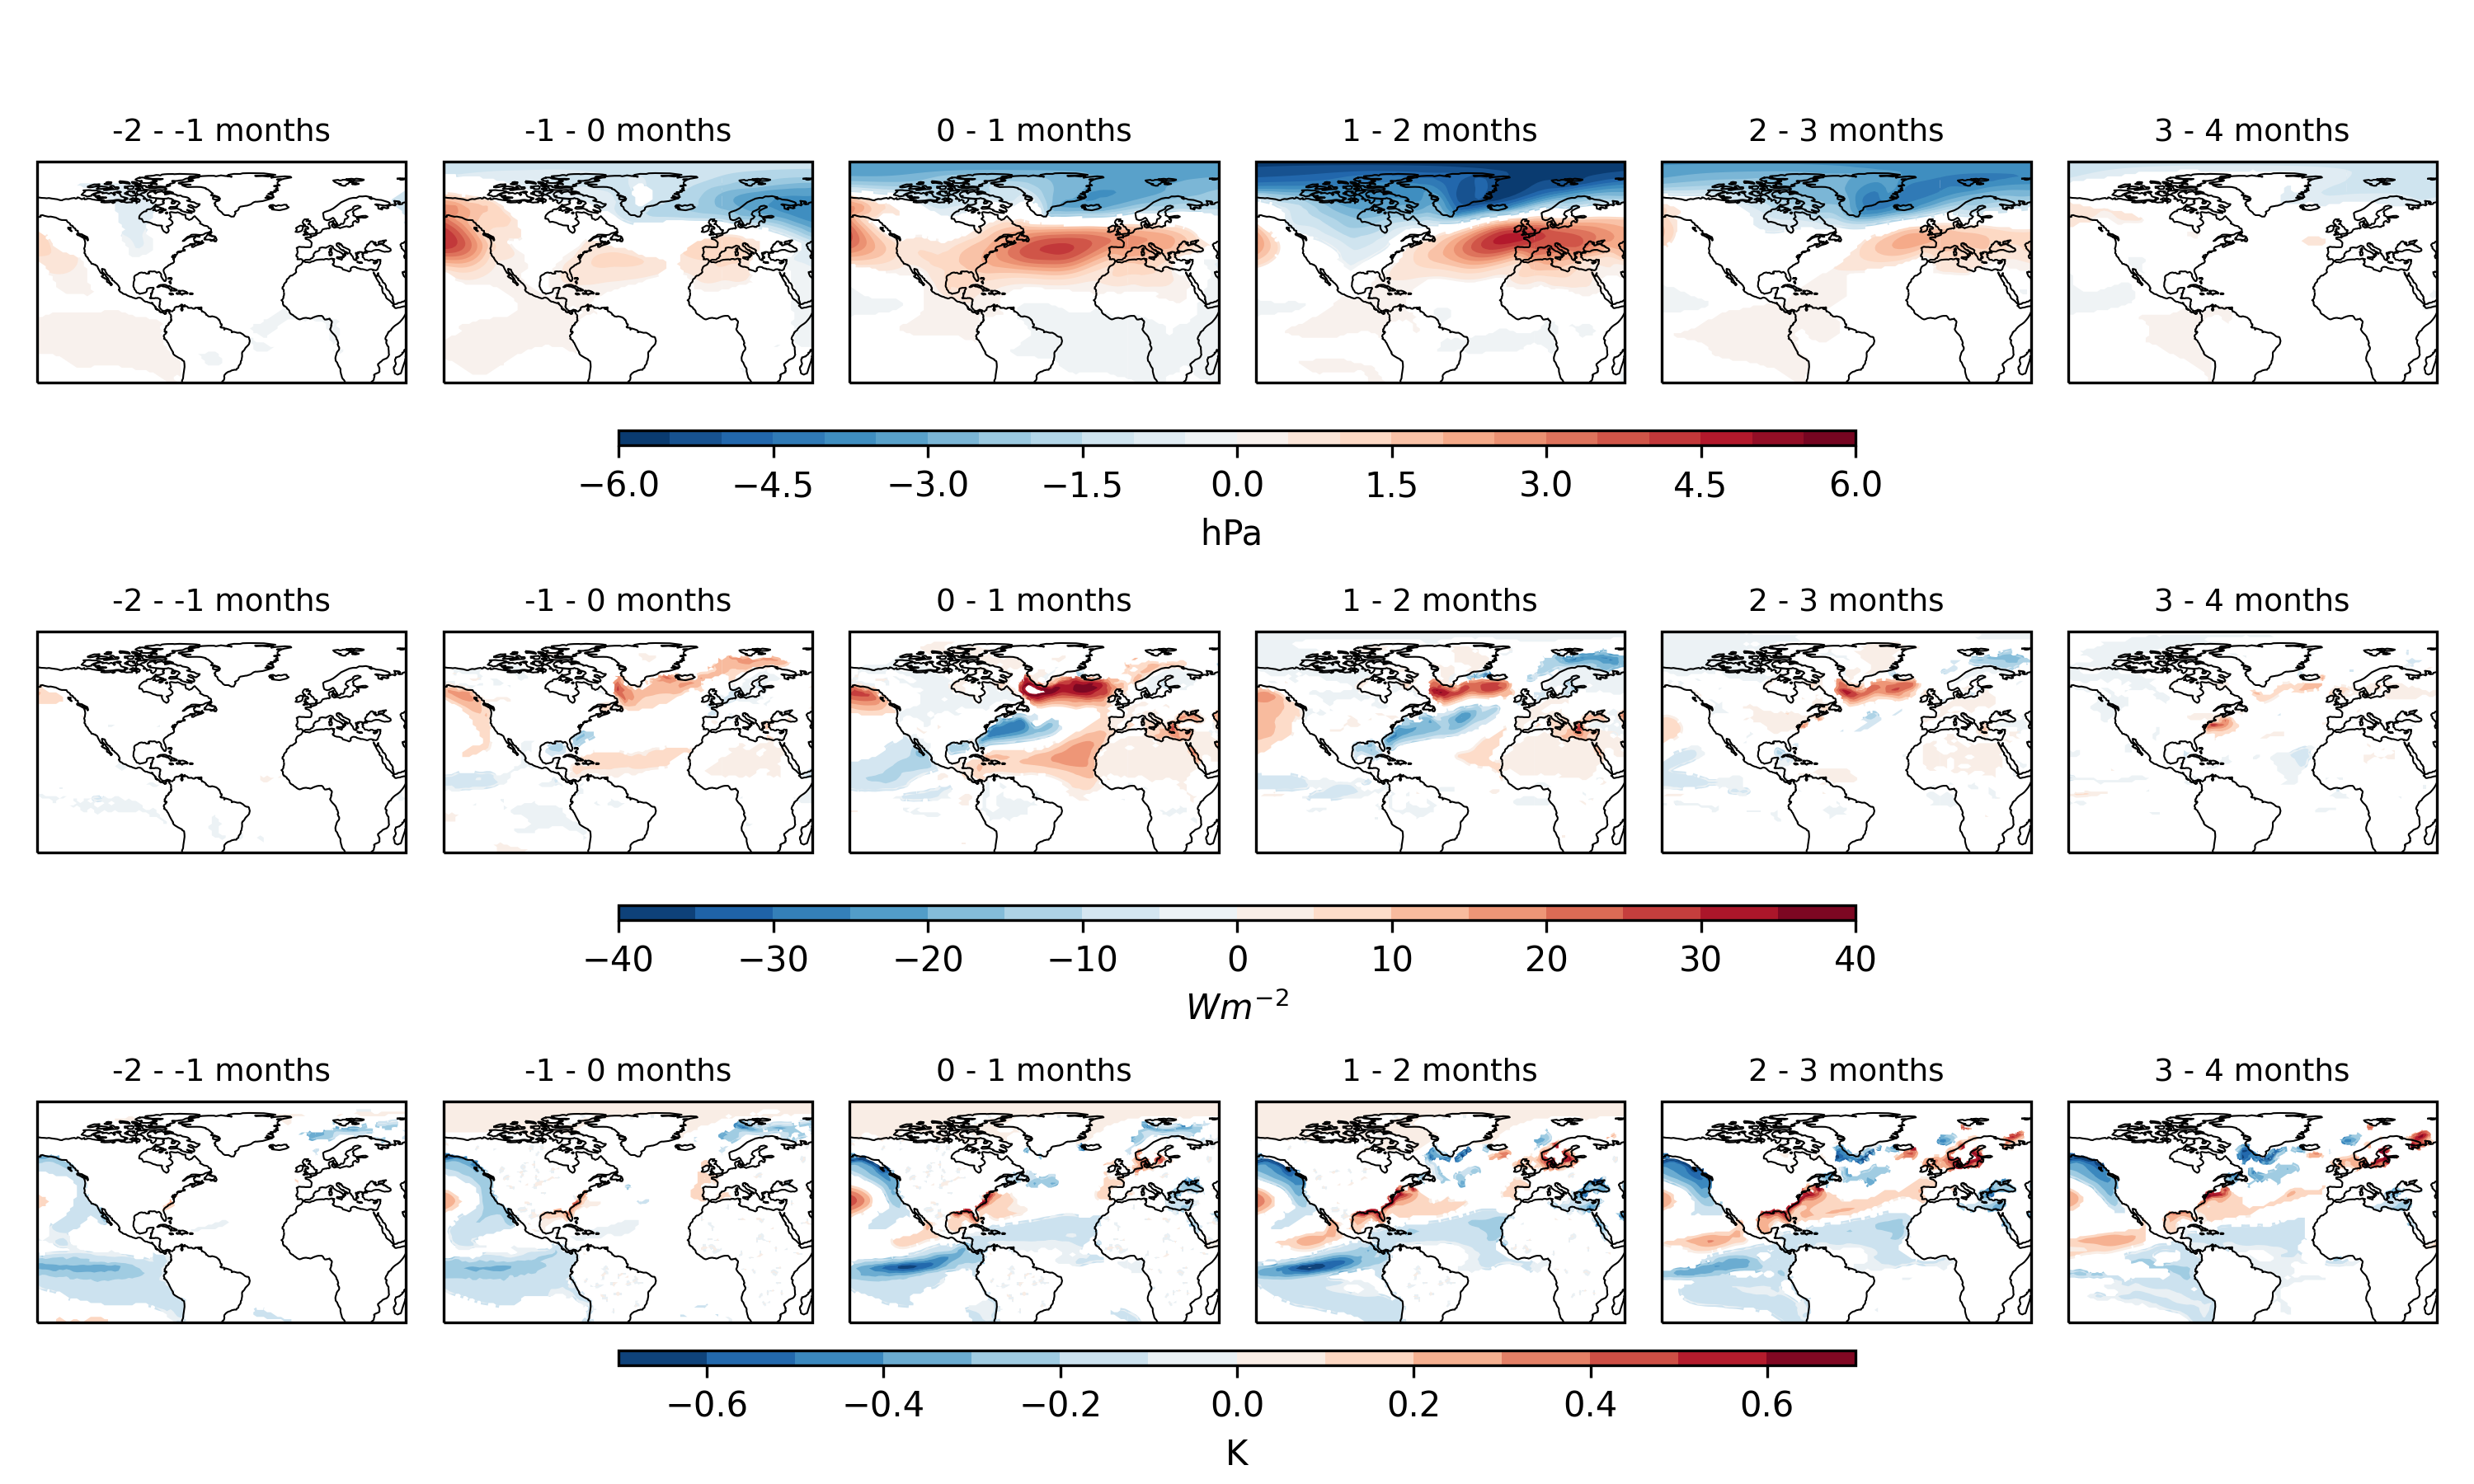
\includegraphics[width = \linewidth]{Figures/Figures-surface/in_season_response_NAM_combined.png}
\caption{Surface patterns associated with anomalous winter stratospheric NAM$_{10}$ events. \textbf{Top row}: Monthly mean sea level pressure anomaly, \textbf{middle row}: Ocean-Atmosphere heat flux defined as the sum of latent and sensible heat fluxes and \textbf{bottom row}: SSTs. Coloured shading shows where the composite differences between strong and weak NAM$_{10}$ events are statistically significant at the 95\% level under a 2 tailed students t-test. The title of each sub-figure indicates the month range relative to the central date of each NAM$_{10}$ anomaly. Signals at negative times indicate that the surface anomaly leads the stratospheric NAM$_{10}$ anomaly. Signals at positive  times indicate that the stratospheric NAM$_{10}$ anomaly leads the surface response.}
\label{fig:surface_comp_all}
\end{figure}
\end{center}

The model also exhibits significant responses in ocean-atmosphere heat flux (figure \ref{fig:surface_comp_all}, middle row). The largest flux anomalies are seen within 30 days (lag 0-1 month) and their spatial pattern resembles that of a North Atlantic tripole with positive anomalies over the Labrador sea and between Greenland and Western Europe, negative anomalies off the east coast of the USA and a second positive anomaly off the coast of north east Africa. This pattern is consistent with the model response found by \cite{reichlerStratospheric2012} to anomalous stratospheric NAM$_{10}$ events as well as the pattern associated with positive NAO phases in \cite{delworthImpact2016}. As with the MSLP composites, there are visible anomalies 30 days leading up to the identified events (lag -1 - 0 months) both over the North Atlantic and Pacific regions. The Atlantic pattern may correspond to early responses to a disrupted or strengthened vortex. The Pacific anomalies preceding events are considerably smaller than the Atlantic anomalies and are concentrated over the Aleutian low region.

The SST response to anomalous stratospheric NAM$_{10}$ events (figure \ref{fig:surface_comp_all}, bottom row) over the North Atlantic lags behind the heat flux anomalies by around 2 months, with the largest amplitude anomalies at around 2-4 month lags.  The anomaly pattern resembles that of the heat flux anomalies (with a change of sign), consistent with a mechanism in which the SSTs respond to the anomalous heat fluxes. A prominent negative tropical East Pacific anomaly is obvious in the months leading up to anomalous vortex events together with  anomalies that resemble the Pacific Decadal Oscillation (PDO) in the region of the Aleutian Low \cite{mantuaPacific1997} and these features persists for several months. Variability in this region is dominated by ENSO variations and a significant body of work has proposed teleconnections between ENSO and vortex strength, consistent with the type of association exhibited here (see section \ref{sec:external_influence_SSTs}), i.e. negative (positive) SSTs or la Ni\~{n}a (el Ni\~{n}o) conditions associated with an anomalously strong (weak) vortex. 

\section{Surface impacts of persistent vortex anomalies}
\label{persistent}
The in-season anomaly patterns associated with anomalous stratospheric NAM$_{10}$ events shown in figure \ref{fig:surface_comp_all} confirm that the model is able to reproduce the observed influence of vortex anomalies at the surface, particularly over the Atlantic region. We now extend the analysis to examine decadal-scale variability. Following the approach of \cite{reichlerStratospheric2012} we smooth the NAM$_{10}$ index  (figure \ref{NAM_and_filtered}) and then select the upper and lower 5 percentiles of this index to identify intervals with a persistent consecutive strong or weak polar vortex (see section \ref{sec:model_diagnostics_surface} for more details). The red and blue dots on figure \ref{NAM_and_filtered} indicate the central year of intervals identified with persistent consecutive vortex anomalies (each dot represents the centre of intervals of at approximately 8 years, see section \ref{sec:model_diagnostics_surface}). Characteristic surface responses associated with these intervals are then analysed by compiling composites of the relevant surface fields for the 80 years surrounding the central year of each positive and negative interval and calculating the (positive minus negative) composite difference. These can then be used to assess the potential surface impacts to observed intervals of persistent consecutive vortex anomalies, such as the consecutive strong anomalies throughout most of the 1990s and the consecutive weak anomalies in the early 2000s. 

\begin{figure}[h!]
\begin{center}
\noindent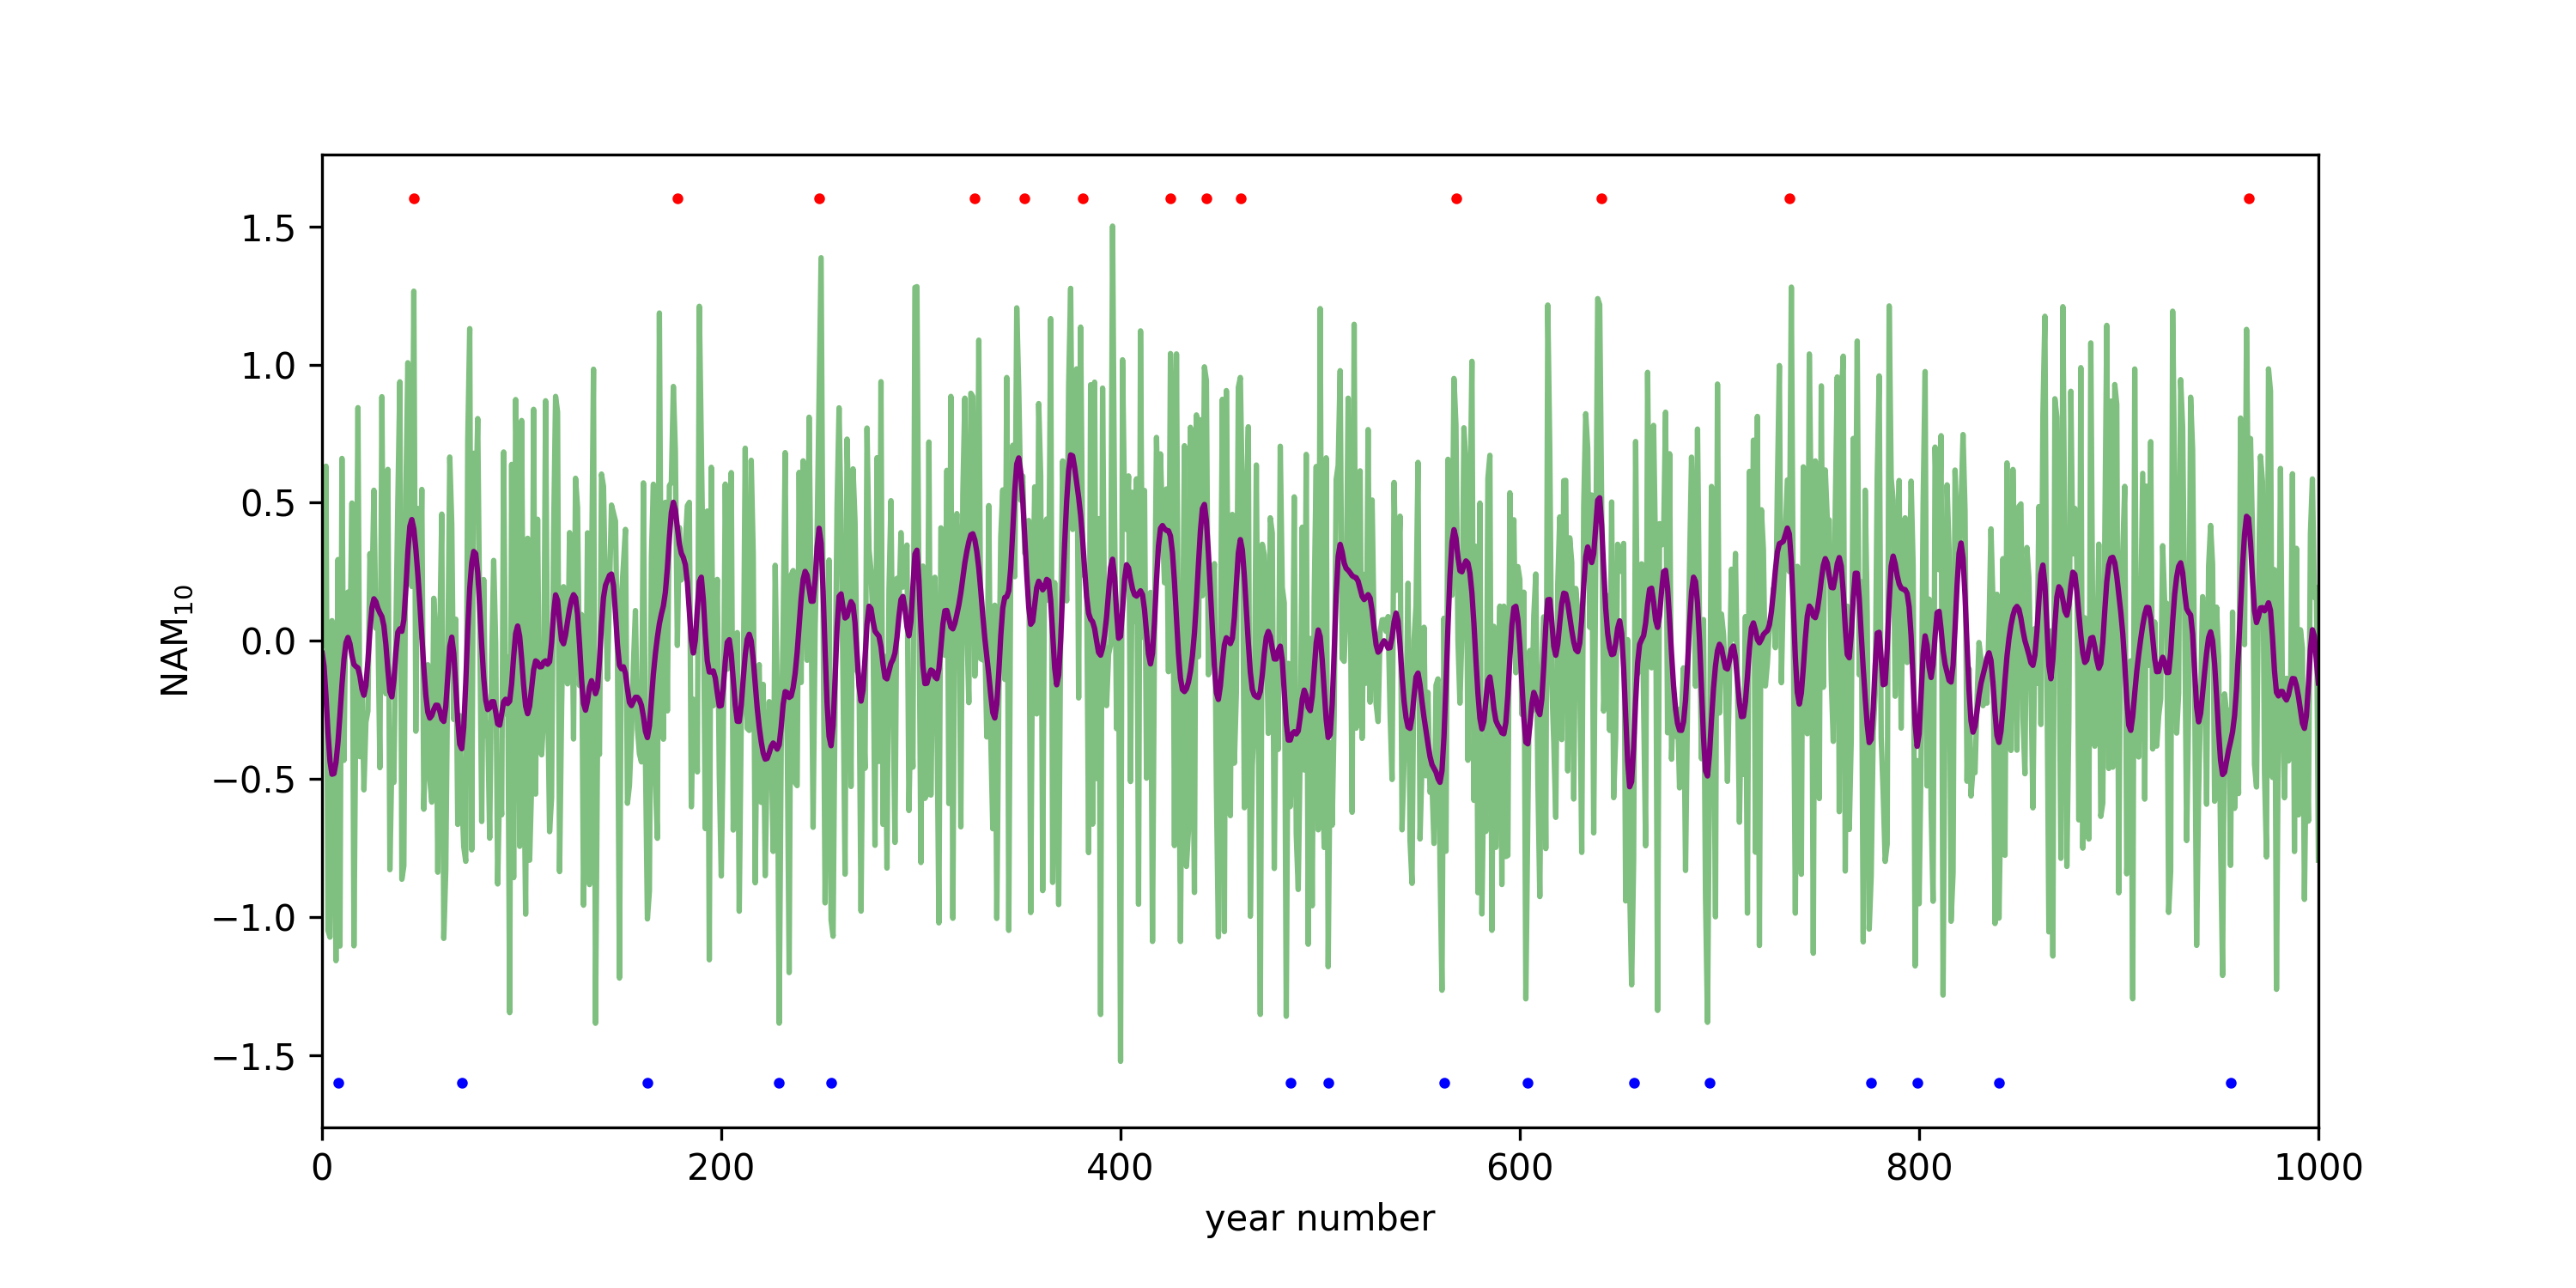
\includegraphics[width = \linewidth]{Figures/Figures-surface/NAM_and_filtered.png} 
\caption{Time series of the December-March mean NAM$_{10}$ index (green) level (\textbf{green}) and smoothed NAM$_{10}$ (purple) evaluated at the 10hPa. The smoothed series is calculated by applying a Gaussian filter ($\sigma = 2$ years) to the green series. Red and blue dots indicate the occurrence of persistent strong and weak vortex intervals respectively defined as extreme values (top and bottom 5 percentiles) in the filtered NAM$_{10}$ index. interval central years are selected such that at least 10 years lies between consecutive intervals.}
\label{NAM_and_filtered}
\end{center}
\end{figure}

A lead-lag analysis of composite differences in the AMOC strength at three different latitudes is shown in  figure \ref{AMOC_comp_NAM}. Positive lags indicate that the stratosphere leads the AMOC response, while negative lags indicate that the AMOC leads the stratospheric response. The figure can be directly compared with figure 4c of \cite{reichlerStratospheric2012}. As found by this work, an oscillatory AMOC response to the stratospheric anomalies is evident, with significant positive anomalies in the AMOC at 45N and 50N at lags of approximately 3-5 years after persistent NAM$_{10}$ intervals followed by negative anomalies at lags between 15 and 20 years. This response pattern is more clearly evident by taking the low pass filtered versions of the AMOC responses (figure \ref{AMOC_comp_NAM}b, d and f) in which we smooth the AMOC index with the same Gaussian filter used to construct the filtered NAM$_{10}$ index. Even after the high frequency signals have been removed, the composite differences still exhibit magnitudes up to 1.5Sv at 15-20 year lags and these are significant under a student's t-test. We note, however, that this low pass filtering of the AMOC time-series reduces the overall variance so that the threshold for a composite difference to pass the significance test is lower, and this may increase the responses that are deemed significant shown in figure \ref{AMOC_comp_NAM}. Nevertheless, given the large magnitude of the response in the filtered AMOC, we conclude that there is evidence of decadal scale variability in the NAM-AMOC interaction and the most significant responses occur when the stratosphere is leading the AMOC. This is in agreement with \cite{reichlerStratospheric2012} who suggest that decadal scale variability in vortex strength acts to amplify a similar timescale of variability in the AMOC through resonance of the two signals. Oscillatory response behaviour is not exhibited clearly by the AMOC at 30N, although negative anomalies at lags of 15-20 years after intervals are still visible. Response patterns at this latitude are also significantly smaller than those at 45N and 50N in the filtered composites (figure \ref{AMOC_comp_NAM}a and b). One possible explanation of this is that the coupling mechanism between the NAM$_{10}$ and AMOC may involve an AMOC response that originates at higher latitudes and then propagates equator-ward therefore exerting less forcing on the AMOC evaluated further south. \cite{zhangLatitudinal2010} also note latitudinal differences in the AMOC response so these differences between 30N, 45N and 50N are not unexpected. The AMOC signals at 45N and 50N also exhibit significant positive anomalies preceding the persistent vortex intervals, at a lead of approximately 20 years and this is also present, albeit smaller in magnitude, in the low pass filtered indices. This precursor to persistent NAM$_{10}$ intervals is not found in corresponding results from \cite{reichlerStratospheric2012} and the role of this feature is considered in more detail in section \ref{surface-strat_forcing}. Overall, these lead-lag difference analyses show that the NAM$_{10}$ and AMOC exhibit elements of co-variability and that decadal scale variations appear to be a key element to this teleconnection. Our results are broadly consistent with similar studies \citep{reichlerStratospheric2012} but with larger responses at lags of 10-20 years.

\begin{center}
\begin{figure}[h!]
\noindent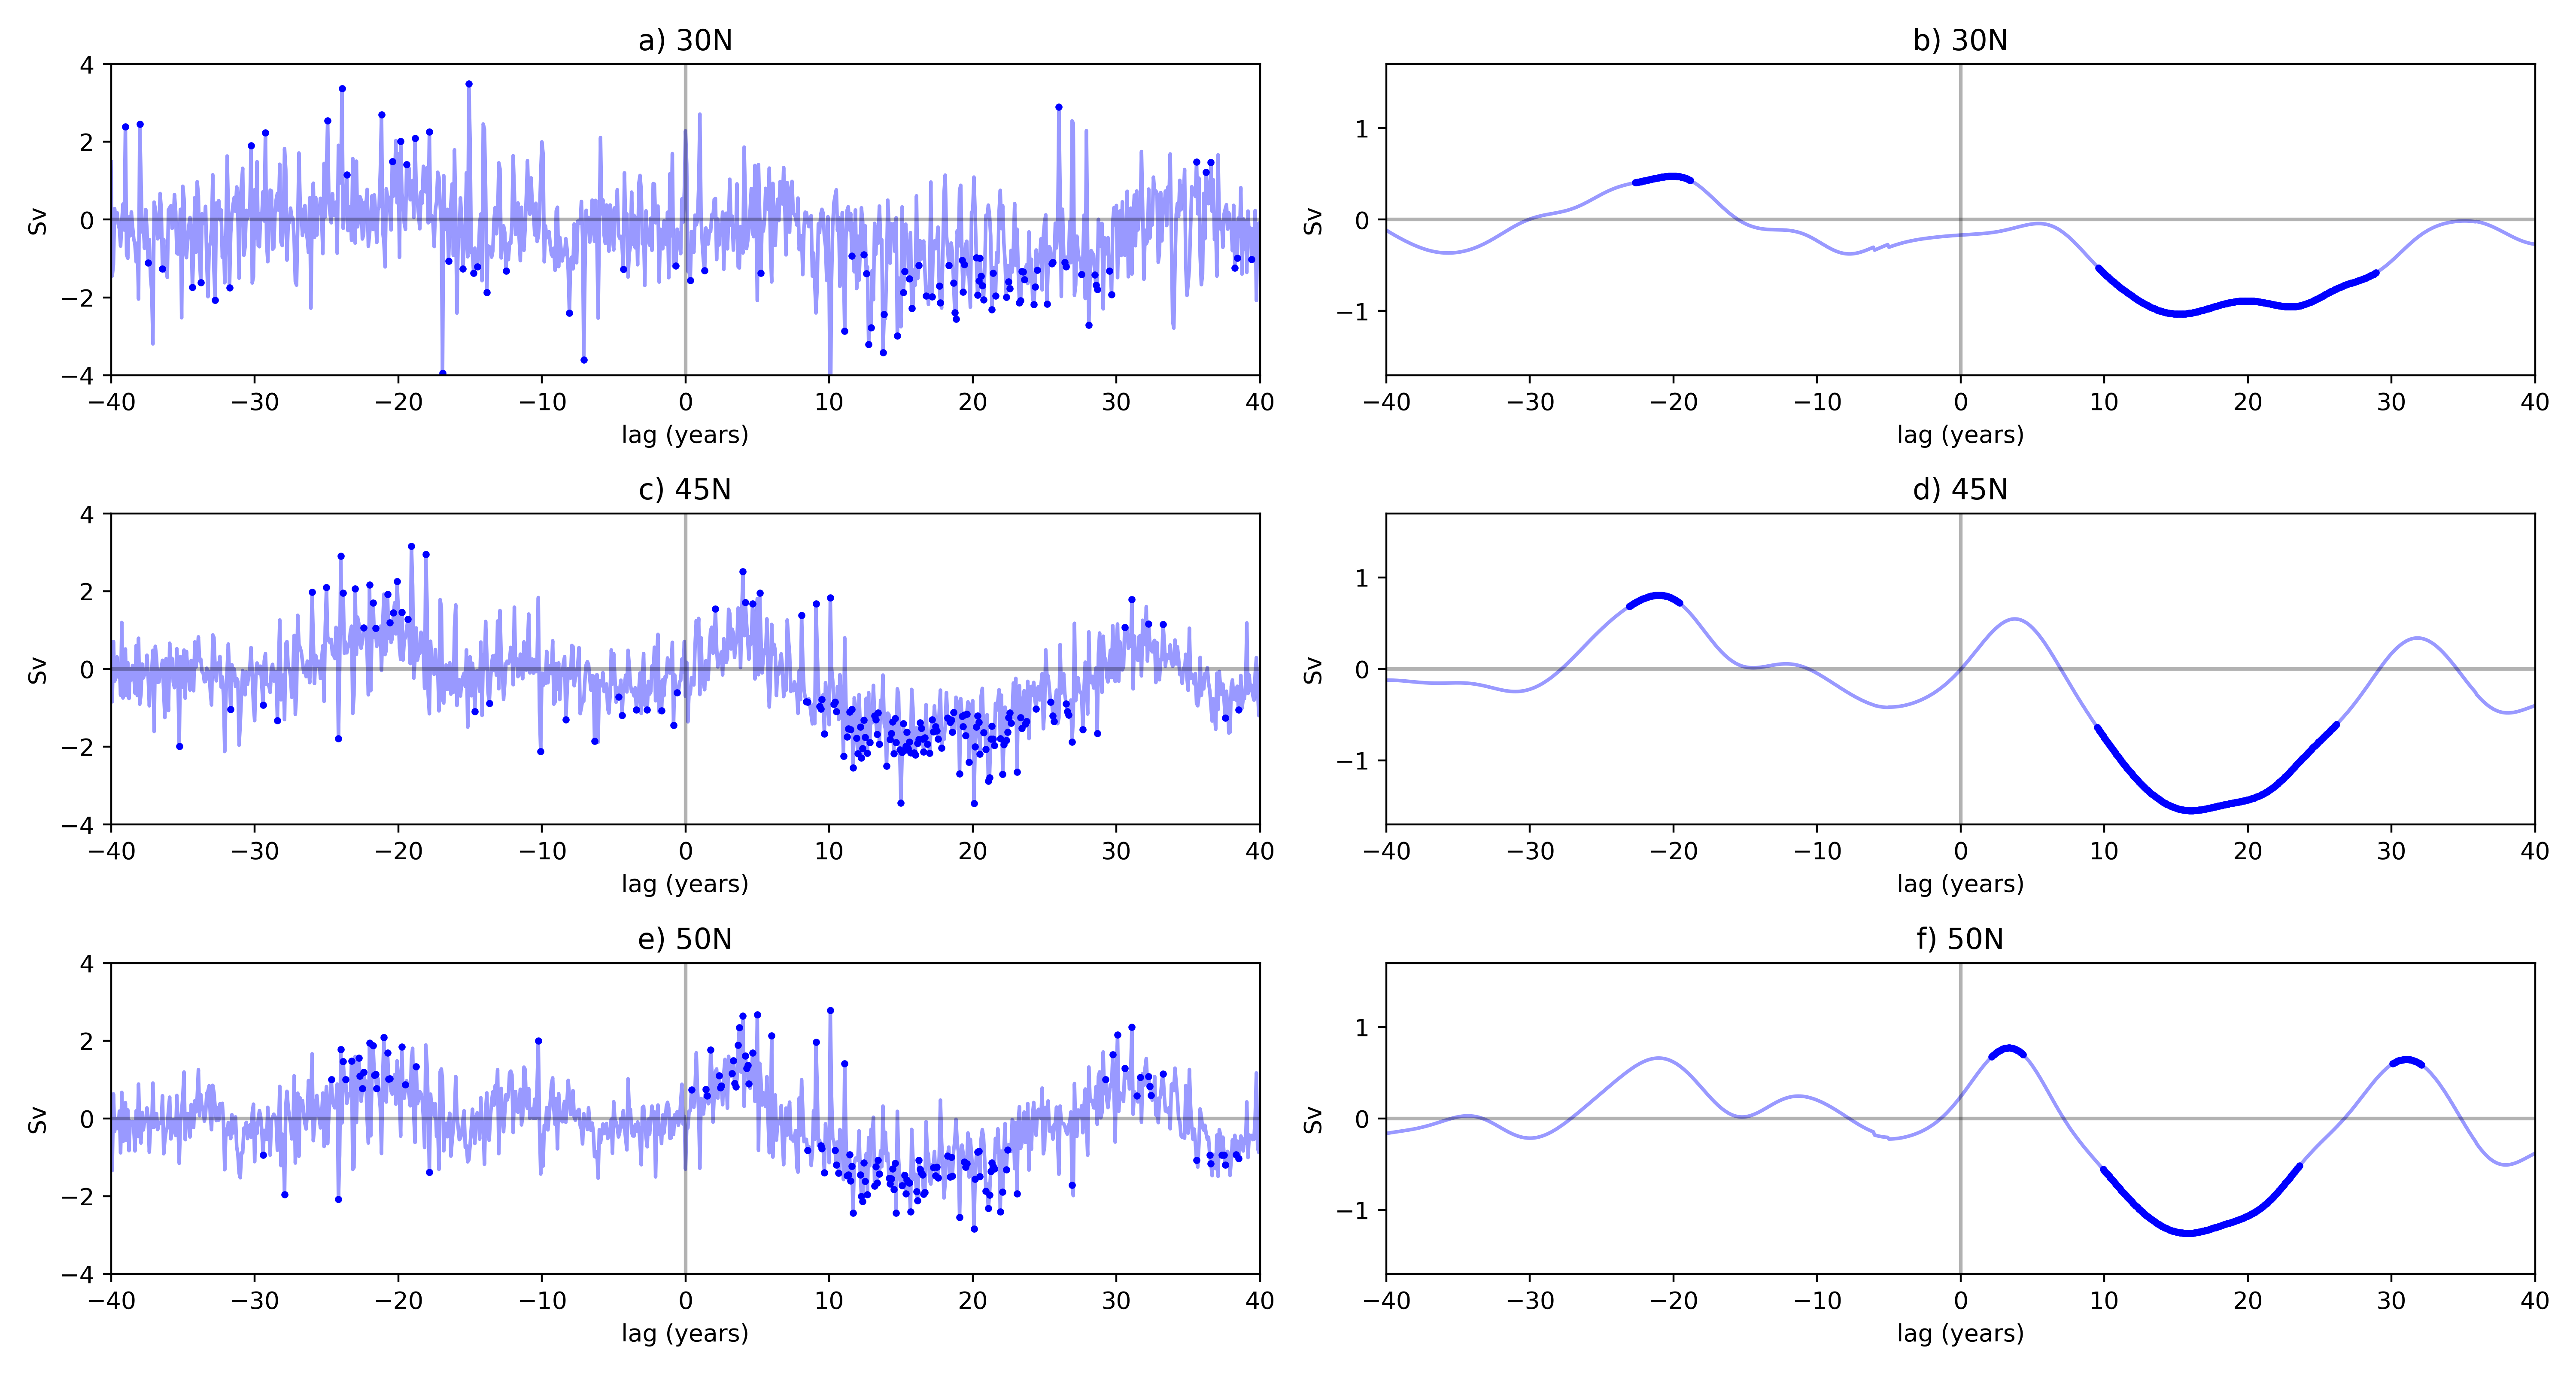
\includegraphics[width = \linewidth]{Figures/Figures-surface/AMOC_responses_low_and_highf_combined.png} 
\caption{Lagged response of AMOC index to persistent NAM$_{10}$ intervals. Blue series shows AMOC composite difference values between positive and negative NAM$_{10}$ intervals defined in section \ref{sec:model_diagnostics_surface}. The $x$ axis denotes the lead (negative values) or lag (positive values) relative to the interval's central year. Black dots denote composite differences significant at the 95\% level under a 2-tailed student's t-test. Panels a, c and e shows monthly AMOC composites which b,d and f show smoothed AMOC composites using a Gaussian filter ($\sigma$ = 2 years).}
\label{AMOC_comp_NAM}
\end{figure}
\end{center}

We now examine this vortex-AMOC teleconnection in closer detail to understand possible physical pathways responsible for an AMOC response to persistent NAM$_{10}$ intervals. figure \ref{NAO_AMOC_T_response}a shows the corresponding lead-lag composite difference analysis for the NAO filtered with the same Gaussian smoother (in green) with the smoothed 50N AMOC response (from fig \ref{AMOC_comp_NAM}f) superimposed for comparison (in blue). There is a zero-lag response in the NH winter NAO, consistent with figure \ref{fig:surface_comp_all} that indicated an in-season NAO response to an anomalous vortex event and the sign of the response is also consistent, with a positive NAO response to persistent positive NAM$_{10}$ anomalies and a negative NAO response to a persistent negative NAM$_{10}$.  There is also a significant negative anomaly in the NAO which emerges at a lag of approximately 10 years and persists up to lags of 18 years. The oscillatory response is also evident, with a positive NAO response at lags of around 28 years but with smaller amplitude than the zero-lag response. 

Also evident from figure \ref{NAO_AMOC_T_response}a is that the oscillatory responses of the NAO and AMOC are similar, with the NAO leading the AMOC response by 2-3 years. Both responses vary with periods of 28-30 years but, interestingly, the negative responses in both signals are  larger and longer-lasting at 10-20 year lags than those at zero and 28-30 year lags. This difference in the magnitude and persistence suggests that the NAO and AMOC response patterns cannot be explained as a straightforward oscillatory response to the NAM$_{10}$ forcing at zero-lag. If this were the case then the response amplitude would be expected to decay with time and the negative response at 10-20 year lag would be smaller than the initial positive response. Instead, a form of feedback mechanism is required to explain the amplified 10-20 year lagged responses or a resonant mechanism as proposed in \cite{reichlerStratospheric2012}. If such a feedback mechanism were present then one might also expect to see some oscillatory behaviour in the smoothed NAM$_{10}$ time-series, in response to the feedback from the surface. To investigate this, figure \ref{NAO_AMOC_T_response}b shows the corresponding lead-lag difference analysis for the NAM$_{10}$ index (i.e. the smoothed NAM$_{10}$ composited around its own extreme values). This supports the presence of a feedback mechanism since it also exhibits oscillatory behaviour with the same period of around 30 years. However, this oscillation is largely evident from the two positive peaks at zero-lag and 30yr-lag, with the latter being substantially damped. There is no significant response at lags of 10-20 years, where the NAO and AMOC responses were largest. This suggests that the negative NAO and AMOC responses at these lags are unlikely to be due to resonance with the NAM$_{10}$ signal. 

Alternatively, a possible physical pathway could involve a two-way amplifying feedback mechanism primarily involving  the NAO and AMOC responses. In this case, the zero-lag NAO response associated with the persistent NAM$_{10}$ intervals would drive a persistent positive ocean-atmosphere heat flux anomaly over the Labrador sea in accordance with the response patterns to individual events seen in figure \ref{fig:surface_comp_all}. This would in turn lead to persistent negative anomalies in the near-surface ocean temperatures as heat is  removed from the ocean via wind stress curl and evaporation. To explore this, figure \ref{AMOC_comp_NAM}c shows the lead-lag difference analysis for the ocean temperatures from the surface to depths of 2000m in a region encompassing the Labrador sea and part of the Central Northern Atlantic (45$^{\circ}$\,–65$^{\circ}$\,N, 15$^{\circ}$\,–60$^{\circ}$\,W). We choose to inspect temperature anomalies in this region as it covers the area over which the majority of Ocean-Atmosphere heat flux responses to individual vortex events appear (figure \ref{fig:surface_comp_all}, middle row). As a result, it is likely to highlight the forcing exerted on the deep ocean via alterations in heat exchange between the atmosphere and the ocean cause by the stratosphere. An identical region is also analysed in \cite{reichlerStratospheric2012}. A near-surface negative response is indeed evident at 0-1yr lags. Subsequently, the AMOC transport would increase due to alterations in density gradients, mixed layer depth and subsequent deep convection in the Labrador sea, an effect discussed in \cite{delworthInterdecadal1993} and \cite{medhaugMechanisms2012}. This accounts for the positive response in the AMOC at 2-3 year lags following NAM$_{10}$ intervals. This increase in AMOC strength would subsequently increases the Labrador Sea temperatures via poleward transport of heat. This is confirmed by the positive, deep (down to 2000m) ocean temperature anomaly at a lag of 10-20 years in figure \ref{NAO_AMOC_T_response}c. In turn, this reversal of the Labrador Sea temperatures can feedback onto the NAO (see e.g. \cite{frankignoulInfluence2013}) by inducing a negative NAO phase at 10 years lags as the increased Labrador Sea heat content alters ocean-atmosphere heat fluxes in the same region.  Finally, this switch in the NAO phase would lead to a subsequent negative AMOC anomaly via the same heat flux mechanism in reverse. This sequence of feedbacks would thus act to enhance the persistence and magnitude of the secondary extreme in the NAO and AMOC. \cite{reichlerStratospheric2012} also briefly suggest a similar mechanism to account for the AMOC response in their simulations, but involving a negative feedback of the AMOC onto itself as well as a role for the NAO. 


\begin{figure}[h!]
\begin{center}
\noindent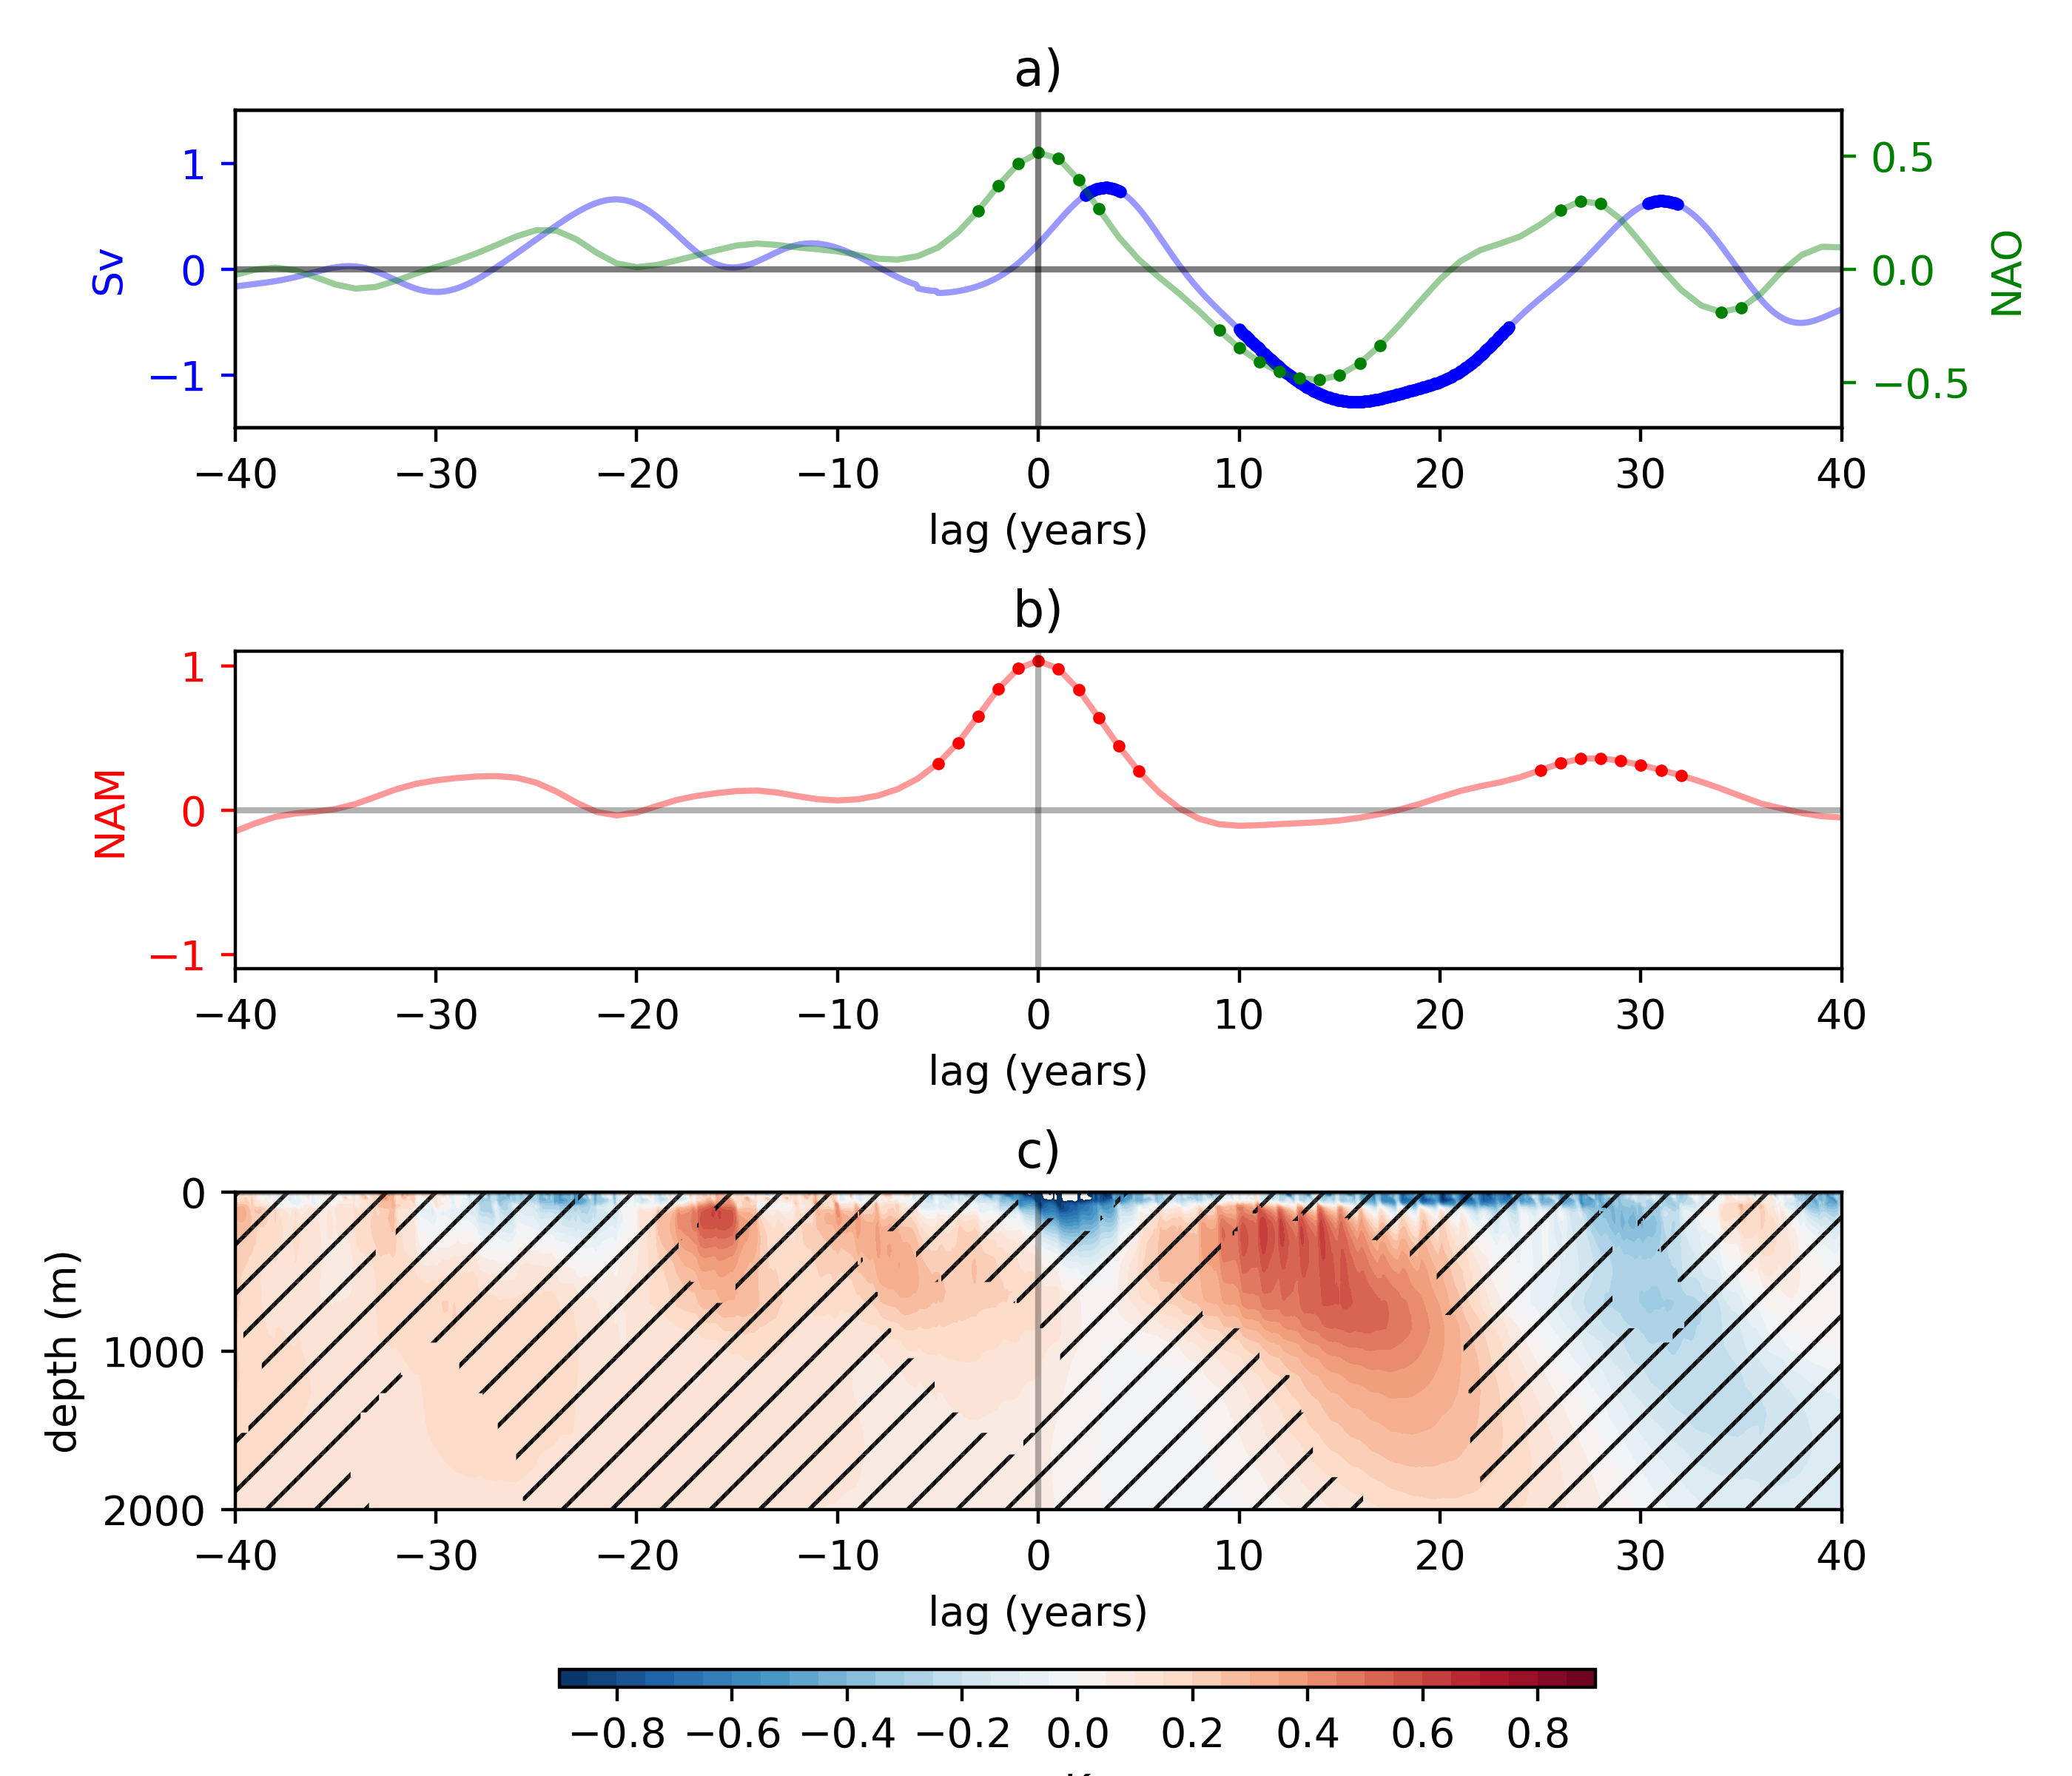
\includegraphics[width = \linewidth]{Figures/Figures-surface/Ocean_T_AMOC_NAO_responses.png} 
\caption{\textbf{a}: Like figure \ref{AMOC_comp_NAM}f for the AMOC at 50N (blue) and the Dec-Mar mean NAO index both smoothed with a Gaussian filter ($\sigma$ = 2 years). \textbf{b}: like \textbf{a} for the smoothed NAM$_{10}$ index around extreme NAM$_{10}$ intervals. \textbf{c}: lagged responses of ocean temperature anomaly depth profiles to persistent NAM$_{10}$ intervals. Composite differences between strong and weak intervals are shown for area weighted averages of an Atlantic box defined by 45$^{\circ}$–65$^{\circ}$N, 15$^{\circ}$–60$^{\circ}$W. Hatching indicates composite differences that are not significant at the 95\% level under a 2-tailed student's t-test.}
\label{NAO_AMOC_T_response}
\end{center}
\end{figure}

So far, we have considered composite difference responses to persistent strong and weak vortex intervals. However, we know that the vortex evolution during strong and weak vortex years is very different and this is likely to lead to differing interactions with surface and ocean variability.  The surface responses to the two extremes are therefore unlikely to be equal and opposite. For example, weak vortex winters are mostly associated with SSWs whose impact at the surface is observed on average 0-60 days after their central date \citep{baldwinStratospheric2001a}. Furthermore,  the vortex often exhibits a pre-conditioned state (see e.g. \cite{charltonNew2007a} and \cite{bancalaPreconditioning2012} outlined in section \ref{sec:SSW}) in which it becomes anomalously strong in the weeks running up to an SSW. So the timing of SSW events within a given season will dictate both the overall strength of the NAM$_{10}$ measured over the winter season (which we use to construct the persistent NAM$_{10}$ index) and the overall strength of the subsequent surface response. In contrast, winters that exhibit an anomalously strong vortex will, on average, exhibit such behaviour throughout the whole season so the impact on the surface will be present for a larger fraction of the winter season.

To assess the separate influences from each type of vortex extreme, figure \ref{NAO_AMOC_response_individual_types} shows the lead-lag composite analysis of the NAO, AMOC and NAM$_{10}$ signals for the persistent positive (strong vortex) and persistent negative (weak vortex) NAM$_{10}$ intervals separately. The AMOC patterns associated with each NAM$_{10}$ type manifest slightly differently. The persistently strong vortex composite shows clear oscillatory behaviour with a period of approximately 28 years. These patterns resemble many of the features observed in the AMOC composite differences associated with persistent NAM$_{10}$ intervals (figure \ref{NAO_AMOC_T_response}a). Specifically, positive AMOC at lags of 2-3 years, negative AMOC at 15-20 years and a second positive anomaly at approximately 30 years. On the other hand, the persistently weak vortex composites exhibit a more complicated response, with double peaked minima at lags of -20 and -11 years and double-peaked maxima at 14 and 25 years. The weak vortex composites also exhibit no significant AMOC response at 2-3 year lags unlike the strong vortex composites. The NAO responses exhibit greater symmetry than those for the AMOC. Both exhibit NAO anomalies at zero-lag followed by an extreme of the opposite sign at approximately 16yr and 14yr lags for strong and weak intervals respectively. As with the AMOC composites, the NAO responses to persistently strong vortex intervals exhibits a pronounced oscillatory behaviour of periods around 28 years. Finally, the corresponding NAM$_{10}$ analysis also shows oscillatory behaviour with periods of around 28 years. (We note that the NAM$_{10}$ results  show statistical significance  at both lead and lag times. However, the lead/lag interpretation is less meaningful in this case since the NAM$_{10}$ is used both as the signal and in the selection of the composites. The significance at both lead and lag times simply confirms that there is oscillatory behaviour). 

The asymmetry between the AMOC and NAO responses to persistently strong and persistently weak vortex intervals and the complexity of the separate responses show that the interactions between the NAM$_{10}$ and these surface modes are complex, with some suggestion of oscillatory behaviour on different timescales. In the following sections we address these complexities in more detail by analysing the frequency spectra of the time-series and show that some of these complexities can be explained in terms of the non-stationarity of the signals.

\begin{figure}[h!]
\begin{center}
\noindent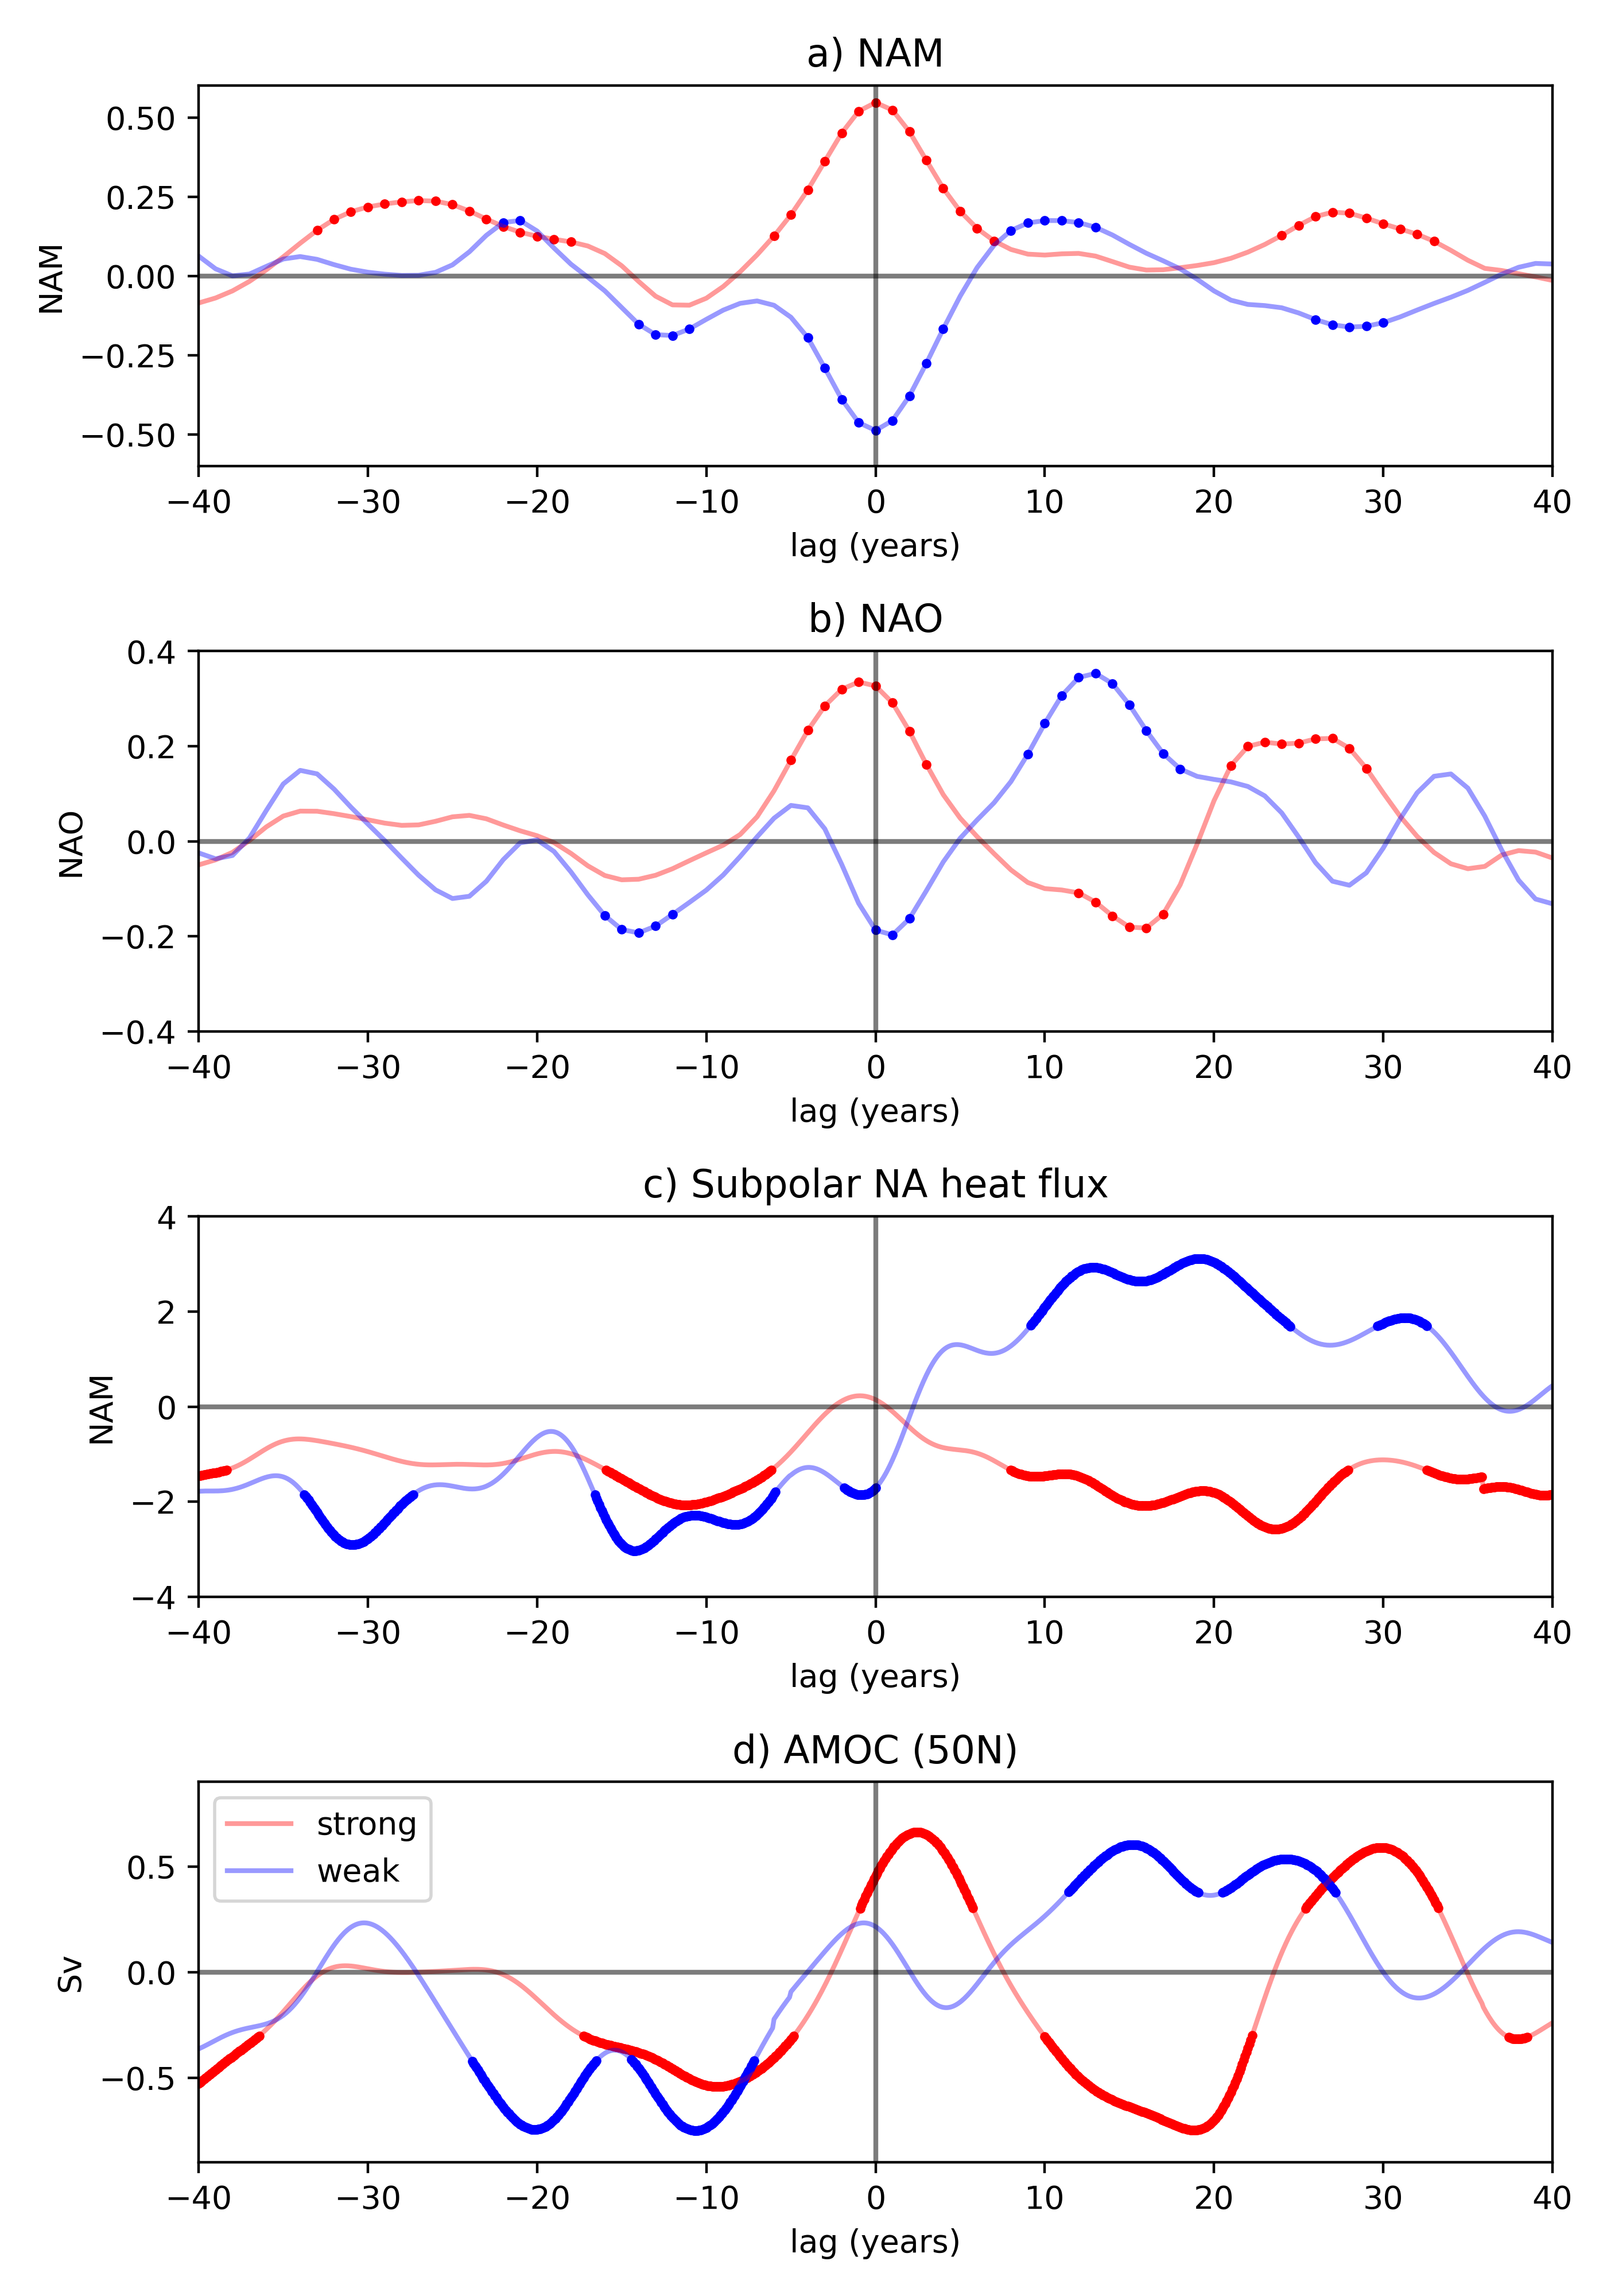
\includegraphics[width =\linewidth]{Figures/Figures-surface/AMOC_NAO_NAM_responses_each_event_type.png} 
\caption{\textbf{a}: Composites of Gaussian smoothed AMOC anomalies at 50N (a), NAO (b) and NAM$_{10}$ (c) associated with persistent vortex intervals of different types. On each sub-figure red (blue) series represent composites about strong (weak) persistent NAM$_{10}$ intervals. Solid dots denote composite anomalies significant to the 95\% level under a 2-tailed student's t-test.}
\label{NAO_AMOC_response_individual_types}
\end{center}
\end{figure}

\section{Non-Stationary Variability}
The analysis of chapter 3 showed that variability of the stratospheric polar vortex occurs on a range of timescales and is highly non-stationary (figure \ref{fig:SSW_series_5yr_wavelet}). Although the composite analysis presented above shows oscillatory behaviour with periods of approximately 30-yr the results are likely complicated by the presence of  non-stationary variability at other periodicities. We therefore analyse the frequency characteristics of the filtered NAM$_{10}$ index. Figure \ref{NAM_wavelet} shows the wavelet power spectrum of this index. It reveals variability on a range of timescales. As expected from the composite analyses, the spectrum exhibits intermittent power throughout the whole simulation at periods between 15 and 40 years. There is also significant power corresponding to a period of approximately 90-100 years that persists for $\sim$300 years of the simulation (year numbers 520-820; approximately 3 cycles) as well as power at the 50 year period timescale that persists for 120 years (year numbers 500-620; approximately 2 cycles). These features are similar to those exhibited by the SSW$_5yr$ timeseries analysis of chapter 3 but not identical, since their time-series was a measure of SSW frequency whereas figure \ref{NAM_wavelet} uses the time-series of smoothed NAM${_10}$ anomaly and therefore provides a measure of persistently strong as well as persistently weak vortex intervals.

The three periodicities  around 30-, 50- and 90-years are also highlighted by the so-called 'global wavelet spectrum' (see figure \ref{NAM_wavelet}), which is an average measure of power over the whole simulation, and shows three peaks in power corresponding to periods of approximately 25, 50 and 90 which are all deemed significant when compared to the spectrum of a theoretical red noise process (see section \ref{sec:Wavelet_Analysis}). We note that much of the $\sim$30-yr periodicity seen in the composite analysis is likely associated with significant wavelet power in the interval between years 300 and 410 and this interval displays the largest number of positive extremes in the smoothed NAM$_{10}$ time-series (compare the 30-yr wavelet power in figure \ref{NAM_wavelet} with the red dots in figure \ref{NAM_and_filtered}). The large number of elevated filtered NAM$_{10}$ extremes selected in this interval is also likely affected by the presence of extremely long timescales variability: qualitative inspection of figure \ref{NAM_and_filtered} shows that the underlying NAM$_{10}$ amplitude increases from around year 200, reaches a peak at $\sim$year 380 and thereafter declines. This means that years within this interval are more likely to reach the top 5 percentile and qualify as an anomalously strong vortex. The origin of this multi-centennial variability is unclear and robust analysis of such a low frequency signal is difficult as the wavelet power is located mostly outside the so called "cone of influence" (blue shading and black hatching on figure \ref{NAM_wavelet}) that marks the boundary at which edge effects become significant. 

\begin{figure}[h!]
\begin{center}
\noindent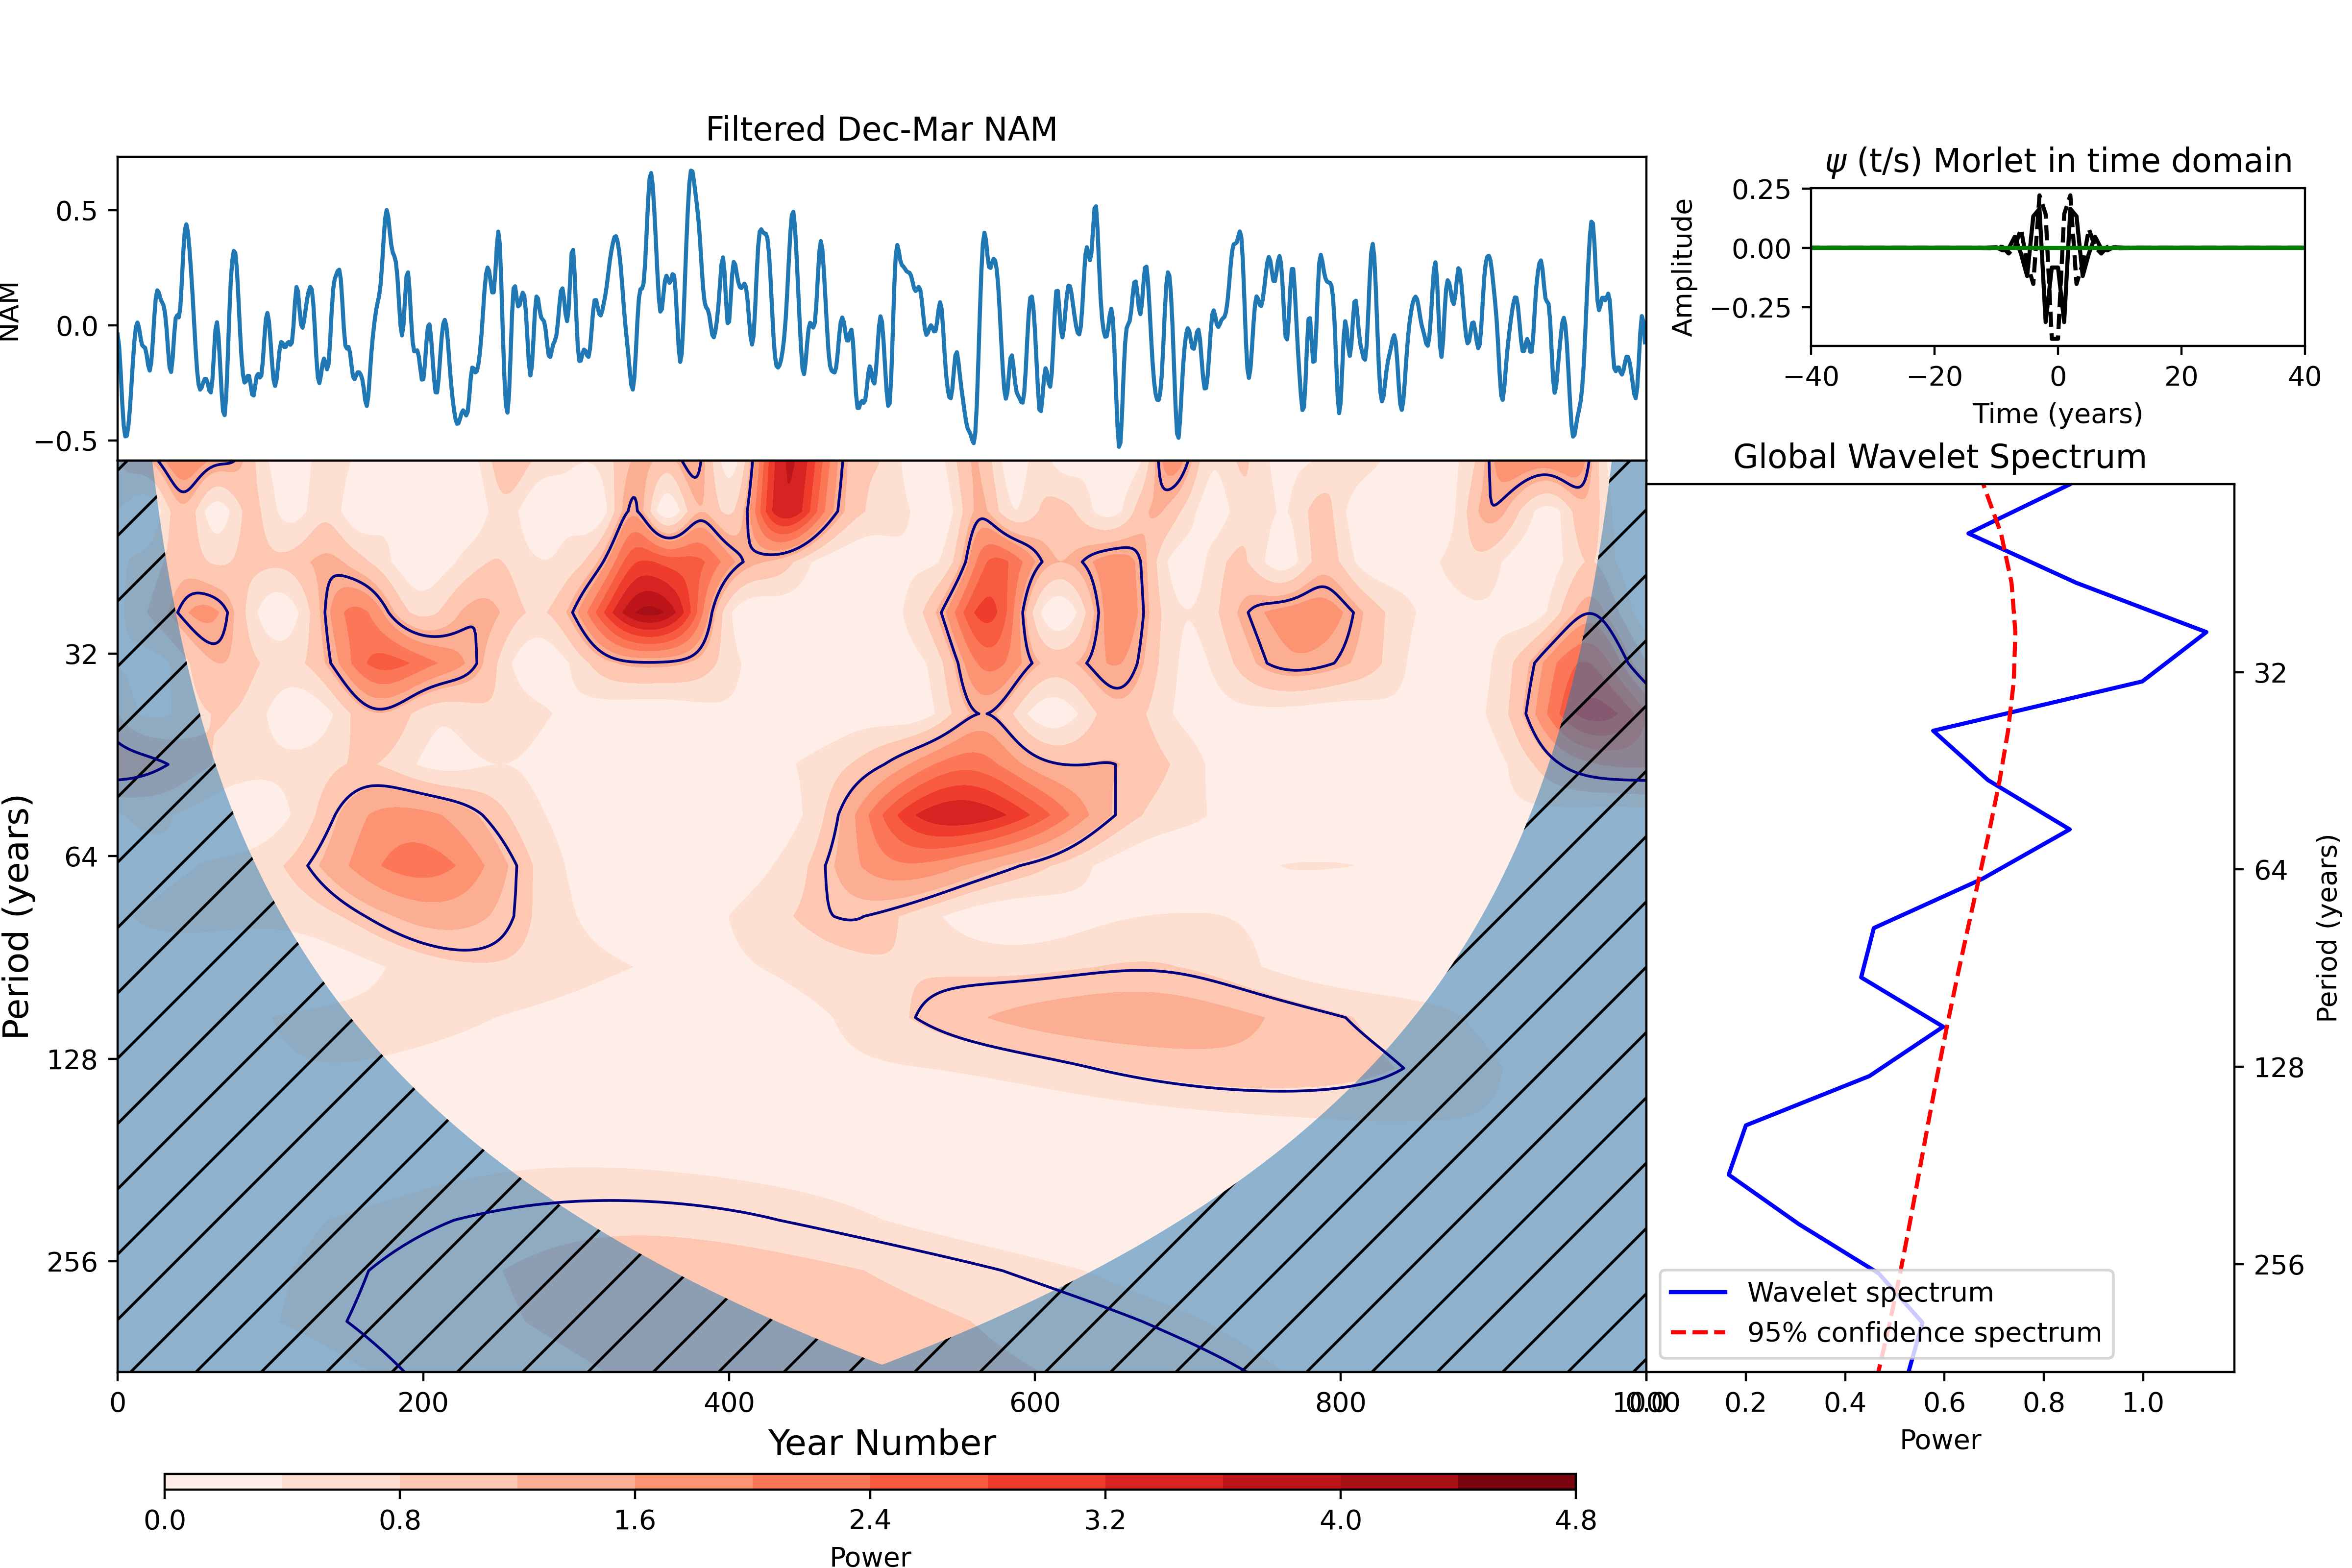
\includegraphics[width = 0.8\linewidth]{Figures/Figures-surface/NAM_wavelet_UKESM.png}
\caption{\textbf{Top left}: Dec-Mar NAM$_{10}$ values smoothed with a with a Gaussian filter ($\sigma$ = 2 years). \textbf{Bottom left}: Wavelet power spectrum of time series in top left. Hatching represents area outside the cone of influence in which edge effects are significant and power should not be considered. Navy contours represent the 95\% confidence level assuming mean background AR1 red noise. \textbf{Top Right}: Morlet wavelet used for the wavelet transform in the time domain. \textbf{Bottom right:} Global power spectrum, the wavelet power averaged over the whole simulation (blue line), and global 95\% confidence spectrum (red dashed line).}
\label{NAM_wavelet}
\end{center}
\end{figure}

A natural question following from the assessment of stratospheric variability in figure \ref{NAM_wavelet} is whether the AMOC variability reflects this? Figure \ref{NAM_AMOC_Cross} shows the corresponding wavelet spectra of the AMOC at 50N and also the cross wavelet spectra between the filtered NAM$_{10}$ and the AMOC which gives a time varying measure of co-variability between signals in the indices at different periods. The wavelet spectrum for the AMOC at 50N exhibits a peak in spectral power corresponding to approximately 130 years that persists for nearly 400 years of the simulation (and also at longer periods up to 250 years but boundary effects are an issue at these multi-centennial timescales, as discussed above). There are also portions of significant power at approximately 30 year and 50 year periods, both of which persist for approximately 2 cycles ($\sim$60 years and $\sim$100 years respectively). These three features are also apparent in the global power spectrum. The 30-yr periodicity is not sustained throughout the whole simulation, so the global power spectrum does not achieve statistical significance at this periodicity, but note that the main 30-yr power comes from the 300-400 year interval, coinciding with the interval of most activity in both the NAM$_{10}$ analysis (figure \ref{NAM_wavelet}) and the selected high NAM$_{10}$ percentiles (figure \ref{NAM_and_filtered}). 
 
The cross power spectrum between the filtered NAM$_{10}$ and the AMOC shows 3 distinct features corresponding broadly to the three timescales prominent on the individual spectra of both indices. Significant cross power is evident at 90-100 year periods for approximately 350 years (between 450 and 800 years; 3-4 cycles). The phase relationship between the signals (indicated by arrows on figure \ref{NAO_NAM_Cross}) within this portion of the cross spectrum  show a mixture of left-pointing arrows in the earlier portion, which indicate an anti-correlated relationship  ($\pi$ out of phase) and downward pointing arrows in the later portion that indicate a $\frac{\pi}{2}$ phase relationship. This latter can be interpreted in a number ways, with maxima in the AMOC leading to maxima in the NAM$_{10}$, minima in the NAM$_{10}$ leading to maxima in the AMOC or maxima in the NAM$_{10}$ index coinciding with maxima in the rate of change of the AMOC (see section \ref{sec:Wavelet_Analysis} for details on cross spectra arrows). There is also significant cross spectral power centred around 30 years (between 300-400 years; 3 cycles) and 50 years (between 500-600 years; 2 cycles). In contrast to the 90-yr periodicity, the phase arrows point to the right and slightly upwards, indicating that maxima in the NAM$_{10}$ index lead to maxima in the AMOC by a small fraction of the cycle. This phase relationship on the 30-yr and 50-yr timescales is consistent with the composite analysis presented in figures \ref{AMOC_comp_NAM} and \ref{NAO_AMOC_response_individual_types} that indicated that a positive (negative) NAM$_{10}$ leads to a positive (negative) AMOC response approximately 2-3 years later. The wavelet spectra for the AMOC at 30N and 45N are provided in figures \ref{NAM_AMOC_Cross_30}a and \ref{NAM_AMOC_Cross_45}a. They show broadly the same features as that of the AMOC at 50N however it is notable that the AMOC at 30N does not exhibit significant variability on the 50 and 30 year timescales. This is reflected in the cross spectrum with the smoothed NAM$_{10}$ index which shows minimal cross power on these timescales (figure \ref{NAM_AMOC_Cross_30}b). This is consistent with figure \ref{AMOC_comp_NAM}b which indicates minimal 30 year timescale modulation of the AMOC at 30N by extremes in the smoothed NAM$_{10}$.

\begin{center}
\begin{figure}[h!]
\noindent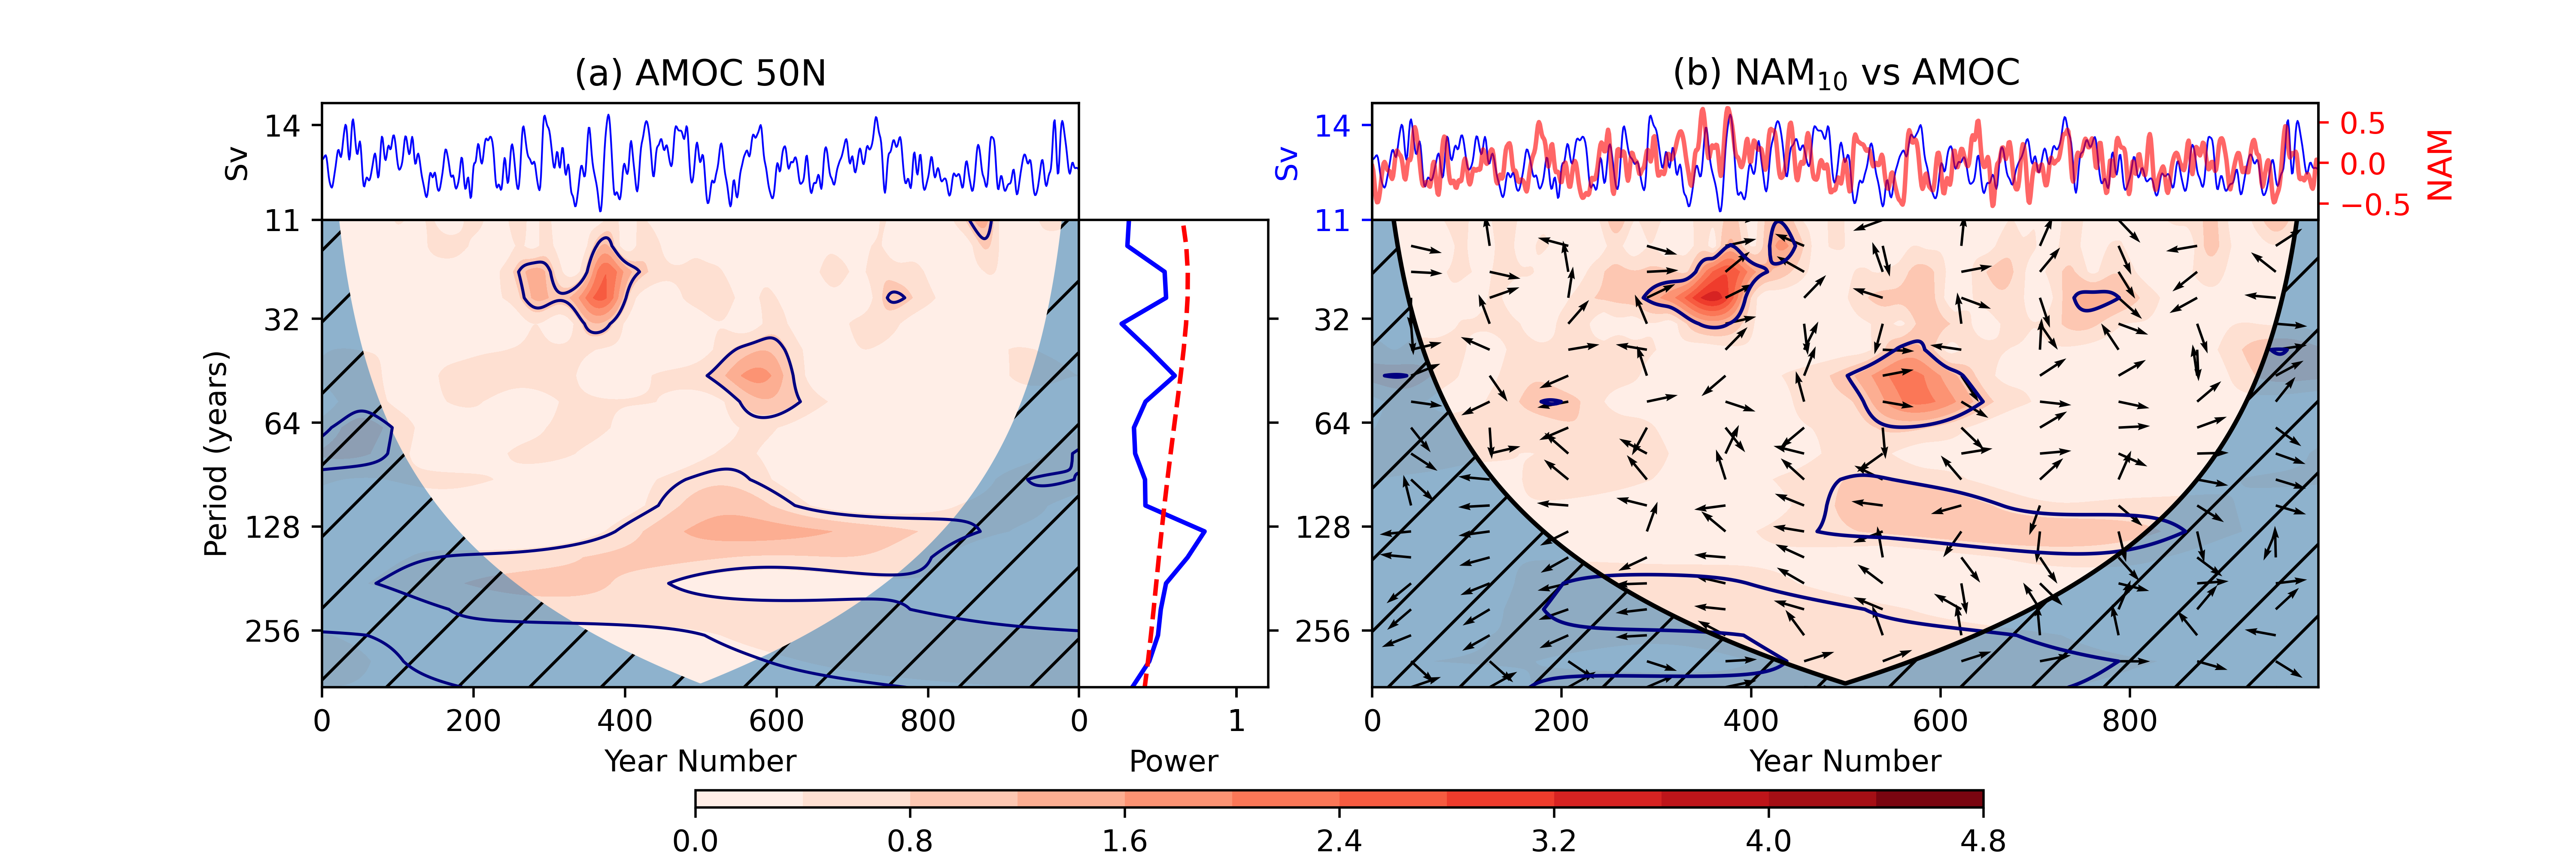
\includegraphics[width = \linewidth]{Figures/Figures-surface/AMOC_NAM_filtered_subplot.png}
\caption{\textbf{(a, top)}: AMOC time series at 50N, \textbf{a, bottom left}: Wavelet power spectrum (shaded contours represent wavelet power and yellow contours the 95\% significance level compared to an AR1 process), \textbf{a, bottom right}: global wavelet power spectrum (blue) and 95\% confidence level (dashed red). \textbf{b}: Cross spectra between Filtered Dec-Mar NAM$_{10}$ series and the AMOC index. \textbf{b, top}: NAM$_{10}$ and AMOC time series. \textbf{b, bottom}: Cross power spectrum. Shading indicates cross power, yellow contours the 95\% confidence interval and arrows the relative phase angle between signals in the time series (to the right: in phase, vertically upwards: $\frac{\pi}{2}$ out of phase with positive peaks in the NAM$_{10}$ leading those in the AMOC, to the left: $\pi$ out of phase, vertically downwards: $\frac{\pi}{2}$ out of phase with positive peaks in the AMOC leading those in the NAM).}
\label{NAM_AMOC_Cross}
\end{figure}
\end{center}

\begin{center}
\begin{figure}[h!]
\noindent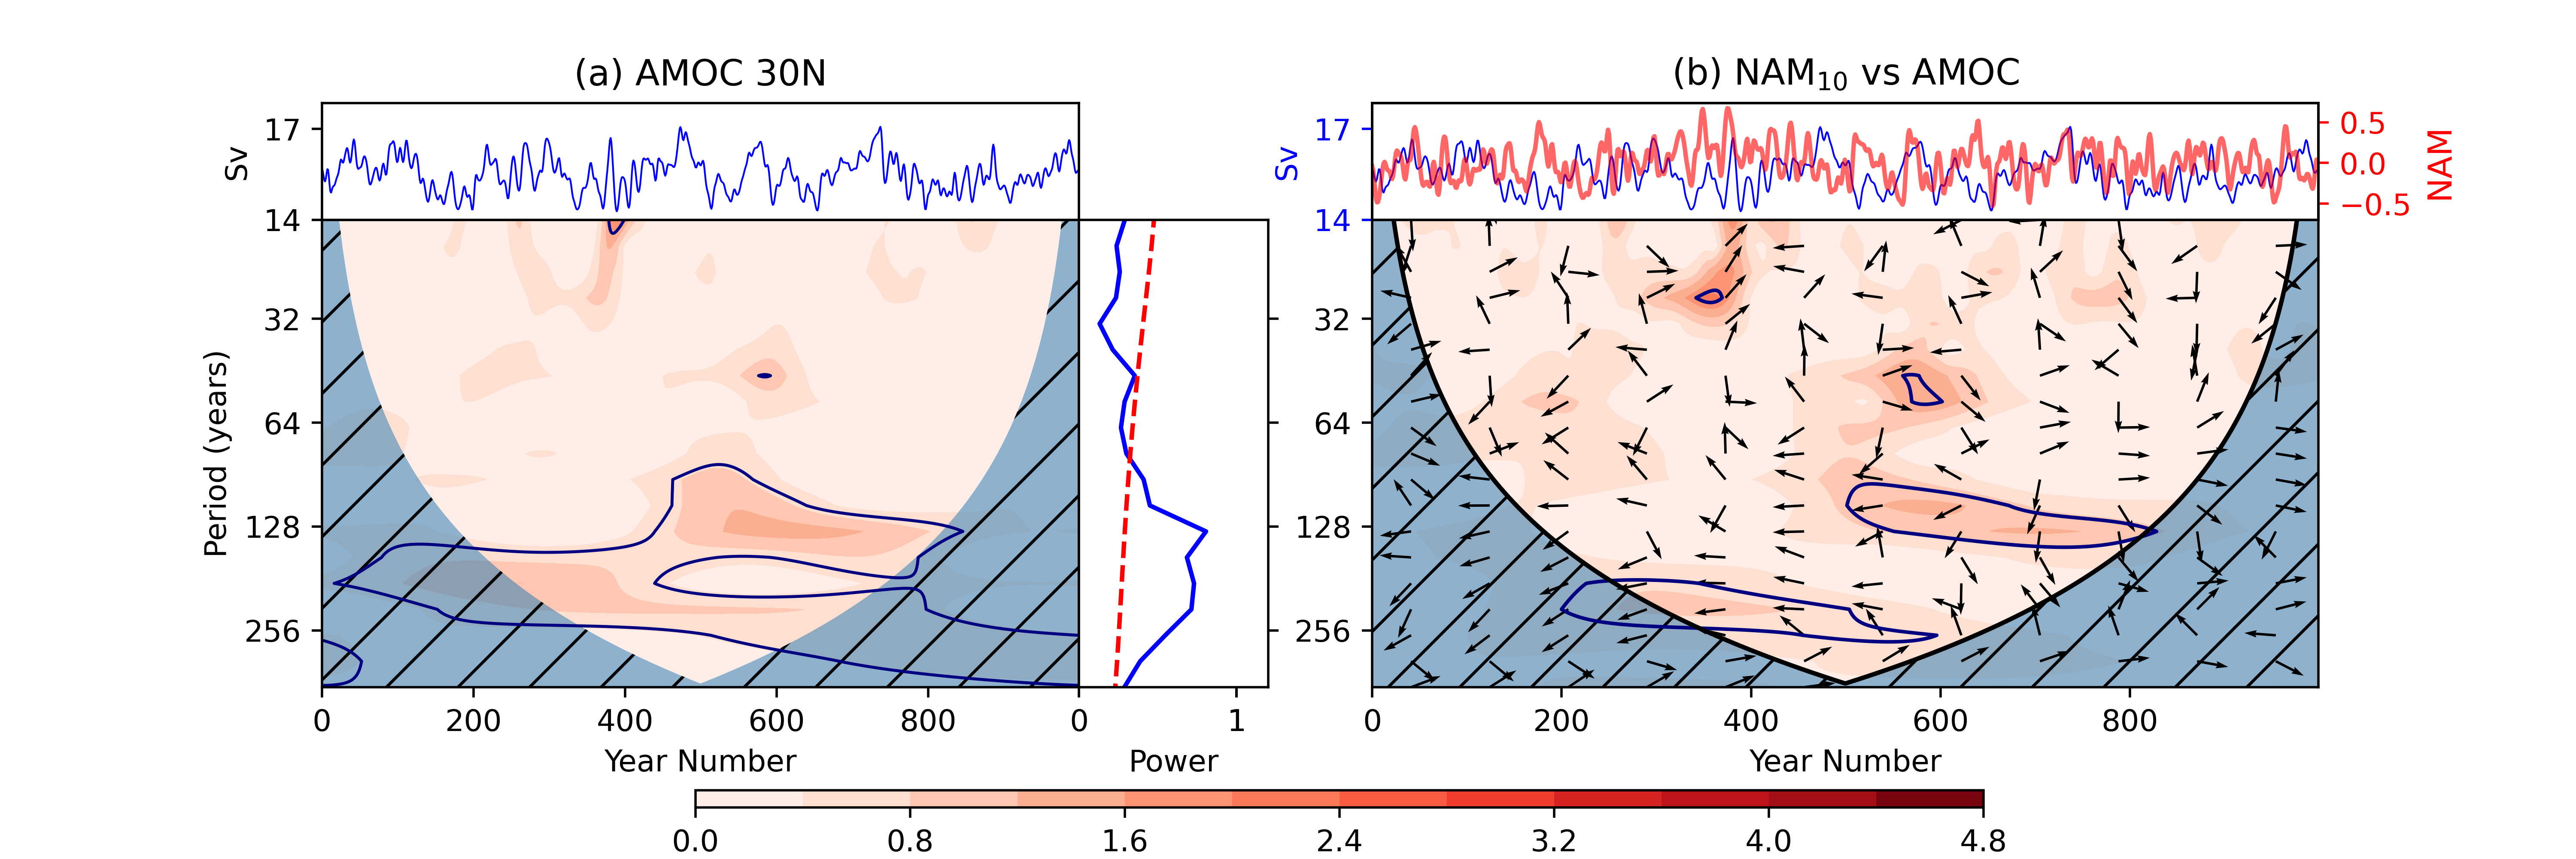
\includegraphics[width = \linewidth]{Figures/Figures-surface/AMOC_NAM_filtered_subplot_30N.png}
\caption{like figure \ref{NAM_AMOC_Cross} for the AMOC at 30N. \textbf{a} shows the wavelet power spectrum of the AMOC and \textbf{b} the cross power spectrum between the AMOC and the NAM$_{10}$ index.}
\label{NAM_AMOC_Cross_30}
\end{figure}
\end{center}

\begin{center}
\begin{figure}[h!]
\noindent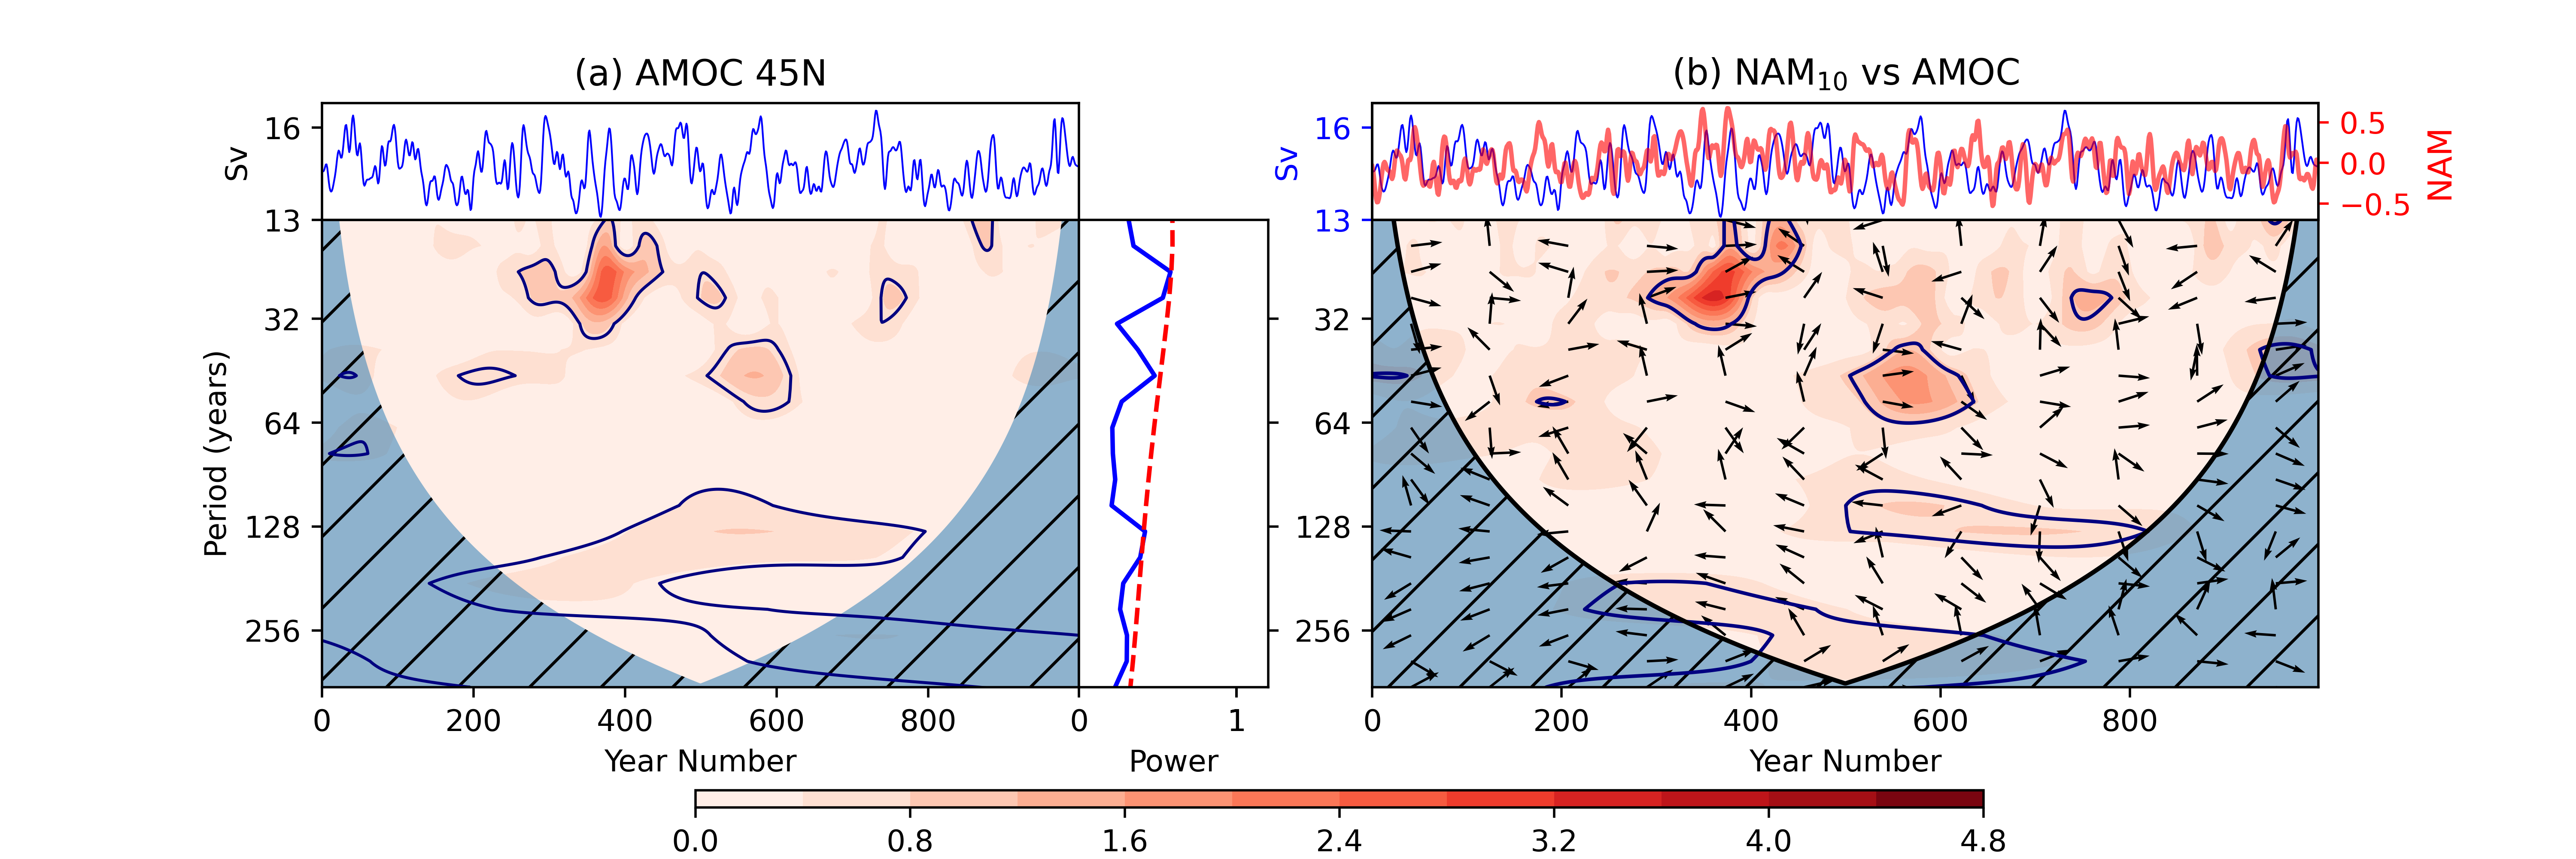
\includegraphics[width = \linewidth]{Figures/Figures-surface/AMOC_NAM_filtered_subplot_45N.png}
\caption{like figure \ref{NAM_AMOC_Cross} for the AMOC at 45N. \textbf{a} shows the wavelet power spectrum of the AMOC and \textbf{b} the cross power spectrum between the AMOC and the NAM$_{10}$ index.}
\label{NAM_AMOC_Cross_45}
\end{figure}
\end{center}
  
To understand these non-stationary signals in the context of the proposed mechanism for vortex-AMOC interactions involving the NAO, we also analyse the power spectrum for the Dec-Mar NAO as well as its cross spectra with the filtered NAM$_{10}$ index (figure \ref{NAO_NAM_Cross}). The wavelet power spectrum for the NAO (figure \ref{NAO_NAM_Cross}a) exhibits some similar features to those of the NAM$_{10}$ and the AMOC. Namely, a portion of significant power at periods of 30 years between $\sim$300-400 years as well as a feature at 50 years between $\sim$500-600 years. Furthermore, the cross power spectrum between the NAO and the NAM$_{10}$ indicate that signals in the two indices on the $\sim$30 and $\sim$50 year periods are also coincident in time for the 70-100 years they persist for. The phase relationship between these signals is small (arrows pointing to the right) indicating an in-phase relationship between the indices, which is consistent with the zero-lag relationship between the NAO and filtered NAM$_{10}$ extremes presented in composite analysis (figures \ref{NAO_AMOC_T_response} and \ref{NAO_AMOC_response_individual_types}). These coincident 30-yr and 50-yr signals between the NAM, AMOC and NAO in these intervals provide supporting evidence for an interaction between these modes of variability. However, the NAO wavelet analysis shows no significant power on the 90-100 year timescale and the prominent feature seen in both the NAM$_{10}$ and AMOC analysis is absent. This suggests that the co-variability between the NAM$_{10}$ and AMOC on these longer timescales does not involve the NAO and is likely to arise through different mechanisms. We return to examine this feature in more detail in section \ref{surface-strat_forcing}.

\begin{figure}[h!]
\begin{center}
\noindent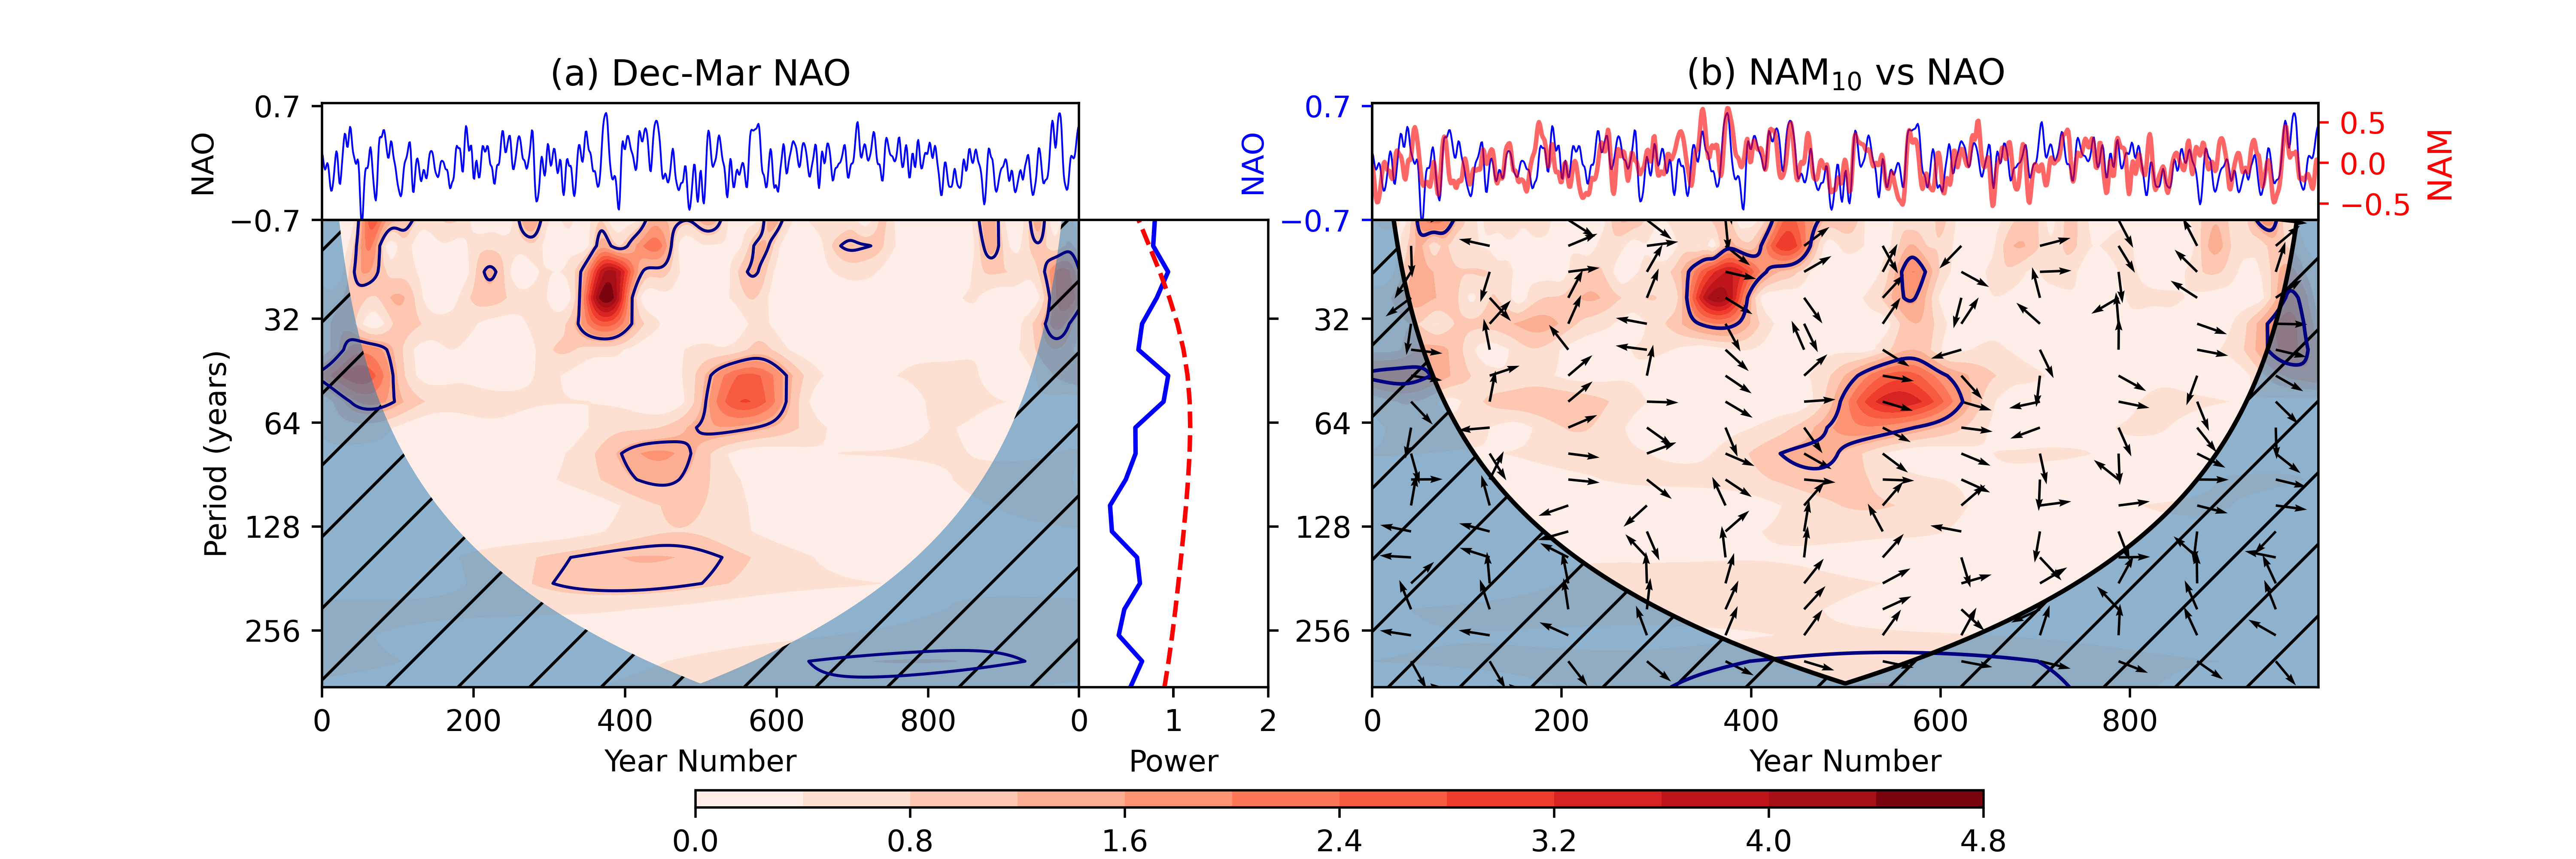
\includegraphics[width = \linewidth]{Figures/Figures-surface/NAM_NAO_filtered_subplot.png}
\caption{like figure \ref{NAM_AMOC_Cross} for the Dec-Mar NAO index. a shows the wavelet power spectrum of the NAO and b the cross power spectrum between the NAO and the NAM$_{10}$ index.}
\label{NAO_NAM_Cross}
\end{center}
\end{figure}

The wavelet analysis suggests that while 30-yr periodicity is most apparent in the composite patterns of figure \ref{NAO_AMOC_T_response} there may also be contributions involving the 50-yr and 90-yr periodicities. This complication is more clearly evident in figure \ref{NAO_AMOC_response_individual_types} where the composites associated with persistent positive and negative NAM$_{10}$ intervals were examined separately. Firstly, we note that the contribution to the composites from the interval exhibiting $\sim$30-year oscillatory behaviour ($\sim$300-400 years) comes solely from a collection of persistent strong NAM$_{10}$ intervals (see the red dots on figure \ref{NAM_and_filtered}). In contrast, a high proportion of the weak NAM$_{10}$ contributions to the composite analysis (8 out of 13) occur within the interval between $\sim$500-600 years which exhibits variability at both 50yr and 90yr periodicity. The complicated double peaked behaviour of the AMOC response following persistent weak vortex intervals can now be better understood, taking into account the influence of the $\sim$50yr and $\sim$90yr periodicities. The double minima in AMOC response at 10yr and 20yr leads and at 15yr and 25yr lags can now be explained as manifestations of the 50-yr and 90-yr AMOC responses e.g. a half-cycle between the minimum at 10yr lead and maximum at 15yr lag (thus a half-cycle of 25 years) gives a periodicity of 50yrs, while a half-cycle between the minimum at 20yr lead and 25yr lag (thus a half-cycle of 45yrs) give a periodicity of 90yrs.  Additional support for this interpretation comes from the fact that the NAO composite analysis (figure 5b) shows a response that corresponds broadly with the AMOC minimum at 10yr lead and maximum at 15yr lag, suggesting a mechanism that involves the NAO on the 50-yr timescale but there is no corresponding response in the NAO at the 90-yr periodicity, in agreement with  the wavelet spectra and cross spectra in figure \ref{NAO_NAM_Cross} which indicates that the NAO does not exhibit variability on timescales of $\sim$90 years. 

\section{Surface Forcing of the Stratosphere}\label{surface-strat_forcing}
The absence of an NAO signal that corresponds to the 90-yr periodicities seen in both the separate NAM$_{10}$ and AMOC wavelet spectra and in the  AMOC-NAM cross spectrum (figure \ref{NAM_AMOC_Cross}) indicates that the mechanism for the stratosphere - AMOC teleconnection on this longer timescale may be distinct in nature to those observed at 30 and 50 year periods. As noted earlier, the phase relationship associated with this feature is also different to the shorter timescales ($\frac{\pi}{2}$ out of phase) suggesting the possibility that the direction of causality may also be switched i.e. it may be that the AMOC leads the stratosphere response on these timescales rather than vice versa. To study this more closely we investigate possible pathways involving variability on this timescale.

In our earlier analysis of this UKESM pi-control simulation from chapter 3 we highlighted the $\sim$90-yr variability in frequency of SSWs and demonstrated that this was closely associated similar timescale variations in the amplitude of the deep QBO (and in particular, the westerly QBO phase).  Figure \ref{OLR_wavelet}a shows the wavelet spectrum of the same QBO index employed in chapter 3 smoothed with the Gaussian filter utilised throughout this work (see \ref{fig:QBO_SSW_subfig}). A portion of significant power at $\sim$90 year periods persists for approximately 200 years of the simulation between years 600-800, which coincides with the significant response in the same interval of the NAM$_{10}$ and AMOC spectra at 90yr periodicity. Cross spectra with the smoothed NAM$_{10}$ index (figure \ref{OLR_wavelet}b) also corroborates the findings from chapter 3 with coincident signals at the 90 year timescales and right-pointing arrows that indicate an in-phase relationship, so that an interval of persistently strong positive (westerly) QBO anomalies  corresponds to an interval of persistent positive (strong) polar vortex intervals (and hence a positive NAM$_{10}$ anomaly). The sign of this teleconnection is consistent with the well-known Holton-Tan teleconnection \citep{luDecadalscale2008, luMechanisms2014c} but it acts on longer timescales and DM21 showed that it originates primarily from long-term variations in the strength of the westerly QBO phase. 

While the long-timescale QBO-vortex teleconnection was demonstrated in chapter 3 (and confirmed here), the cause of the long-term westerly QBO variability was not established. In a preliminary investigation, a wavelet analysis was performed on equatorial SSTs in various regions, including the equatorial East Pacific, to explore whether the $\sim$90-yr QBO variability could be explained via SST triggering of  convective activity that generates the gravity and other equatorial waves that contribute to the QBO. However, no 90-year periodicity in equatorial SSTs was found. A similar analysis of the strength of the Aleutian Low, that could perhaps explain the signals in both the QBO and the polar vortex via a modulation of the strength of large-scale planetary wave forcing, similarly found no periodicity at 90 years. Nevertheless, the extremely long period of the QBO and vortex variations suggest a driving mechanism that is linked to the oceans due to the characteristic long oceanic timescales. 

To extend this investigation, we examine variability of the East Pacific top-of-atmosphere outgoing longwave radiation (OLR) as an alternative proxy for deep convection in the region. When deep convection is enhanced, cloud top height is increased and therefore OLR is reduced. Figure \ref{OLR_wavelet}c shows the wavelet analysis of Sep-Nov  OLR in the East Pacific. It exhibits 90 year periodicity, as well as significant cross power with the smoothed QBO amplitude and the NAM$_{10}$ index (figures \ref{OLR_wavelet}d,e). The signals in the OLR and both the QBO and NAM$_{10}$ are anti-correlated (left pointing arrows indicating a $\pi$ phase difference). This is consistent with reduced OLR (increased deep convection) leading to greater QBO amplitude through increased wave forcing.  The corresponding cross spectra between the AMOC and the OLR metric (figure \ref{OLR_wavelet}f) also indicates a significant portion of cross power in the interval $\sim$600-800 years co-located with the feature seen in the NAM$_{10}$ spectrum (figure \ref{OLR_wavelet} dashed contours). The phase relationship in this case is mostly $\frac{\pi}{2}$ (the majority arrows pointing upwards) indicating that one of the quantities depends on the time rate of change of the other. This relationship is reminiscent of results from \cite{timmermannENSO2005} who show sensitivity of the equatorial Pacific region to 35 year periodic forcing of North Atlantic MOC. Their study showed a dependence of the Pacific thermocline to the rate of change of the AMOC. We therefore suggest this as a possible pathway for 90 year variability in the AMOC to influence the stratospheric NAM, through changes in deep convection in the East Pacific that influences the amplitude of the QBO. 


\begin{figure}[h!]
\begin{center}
\noindent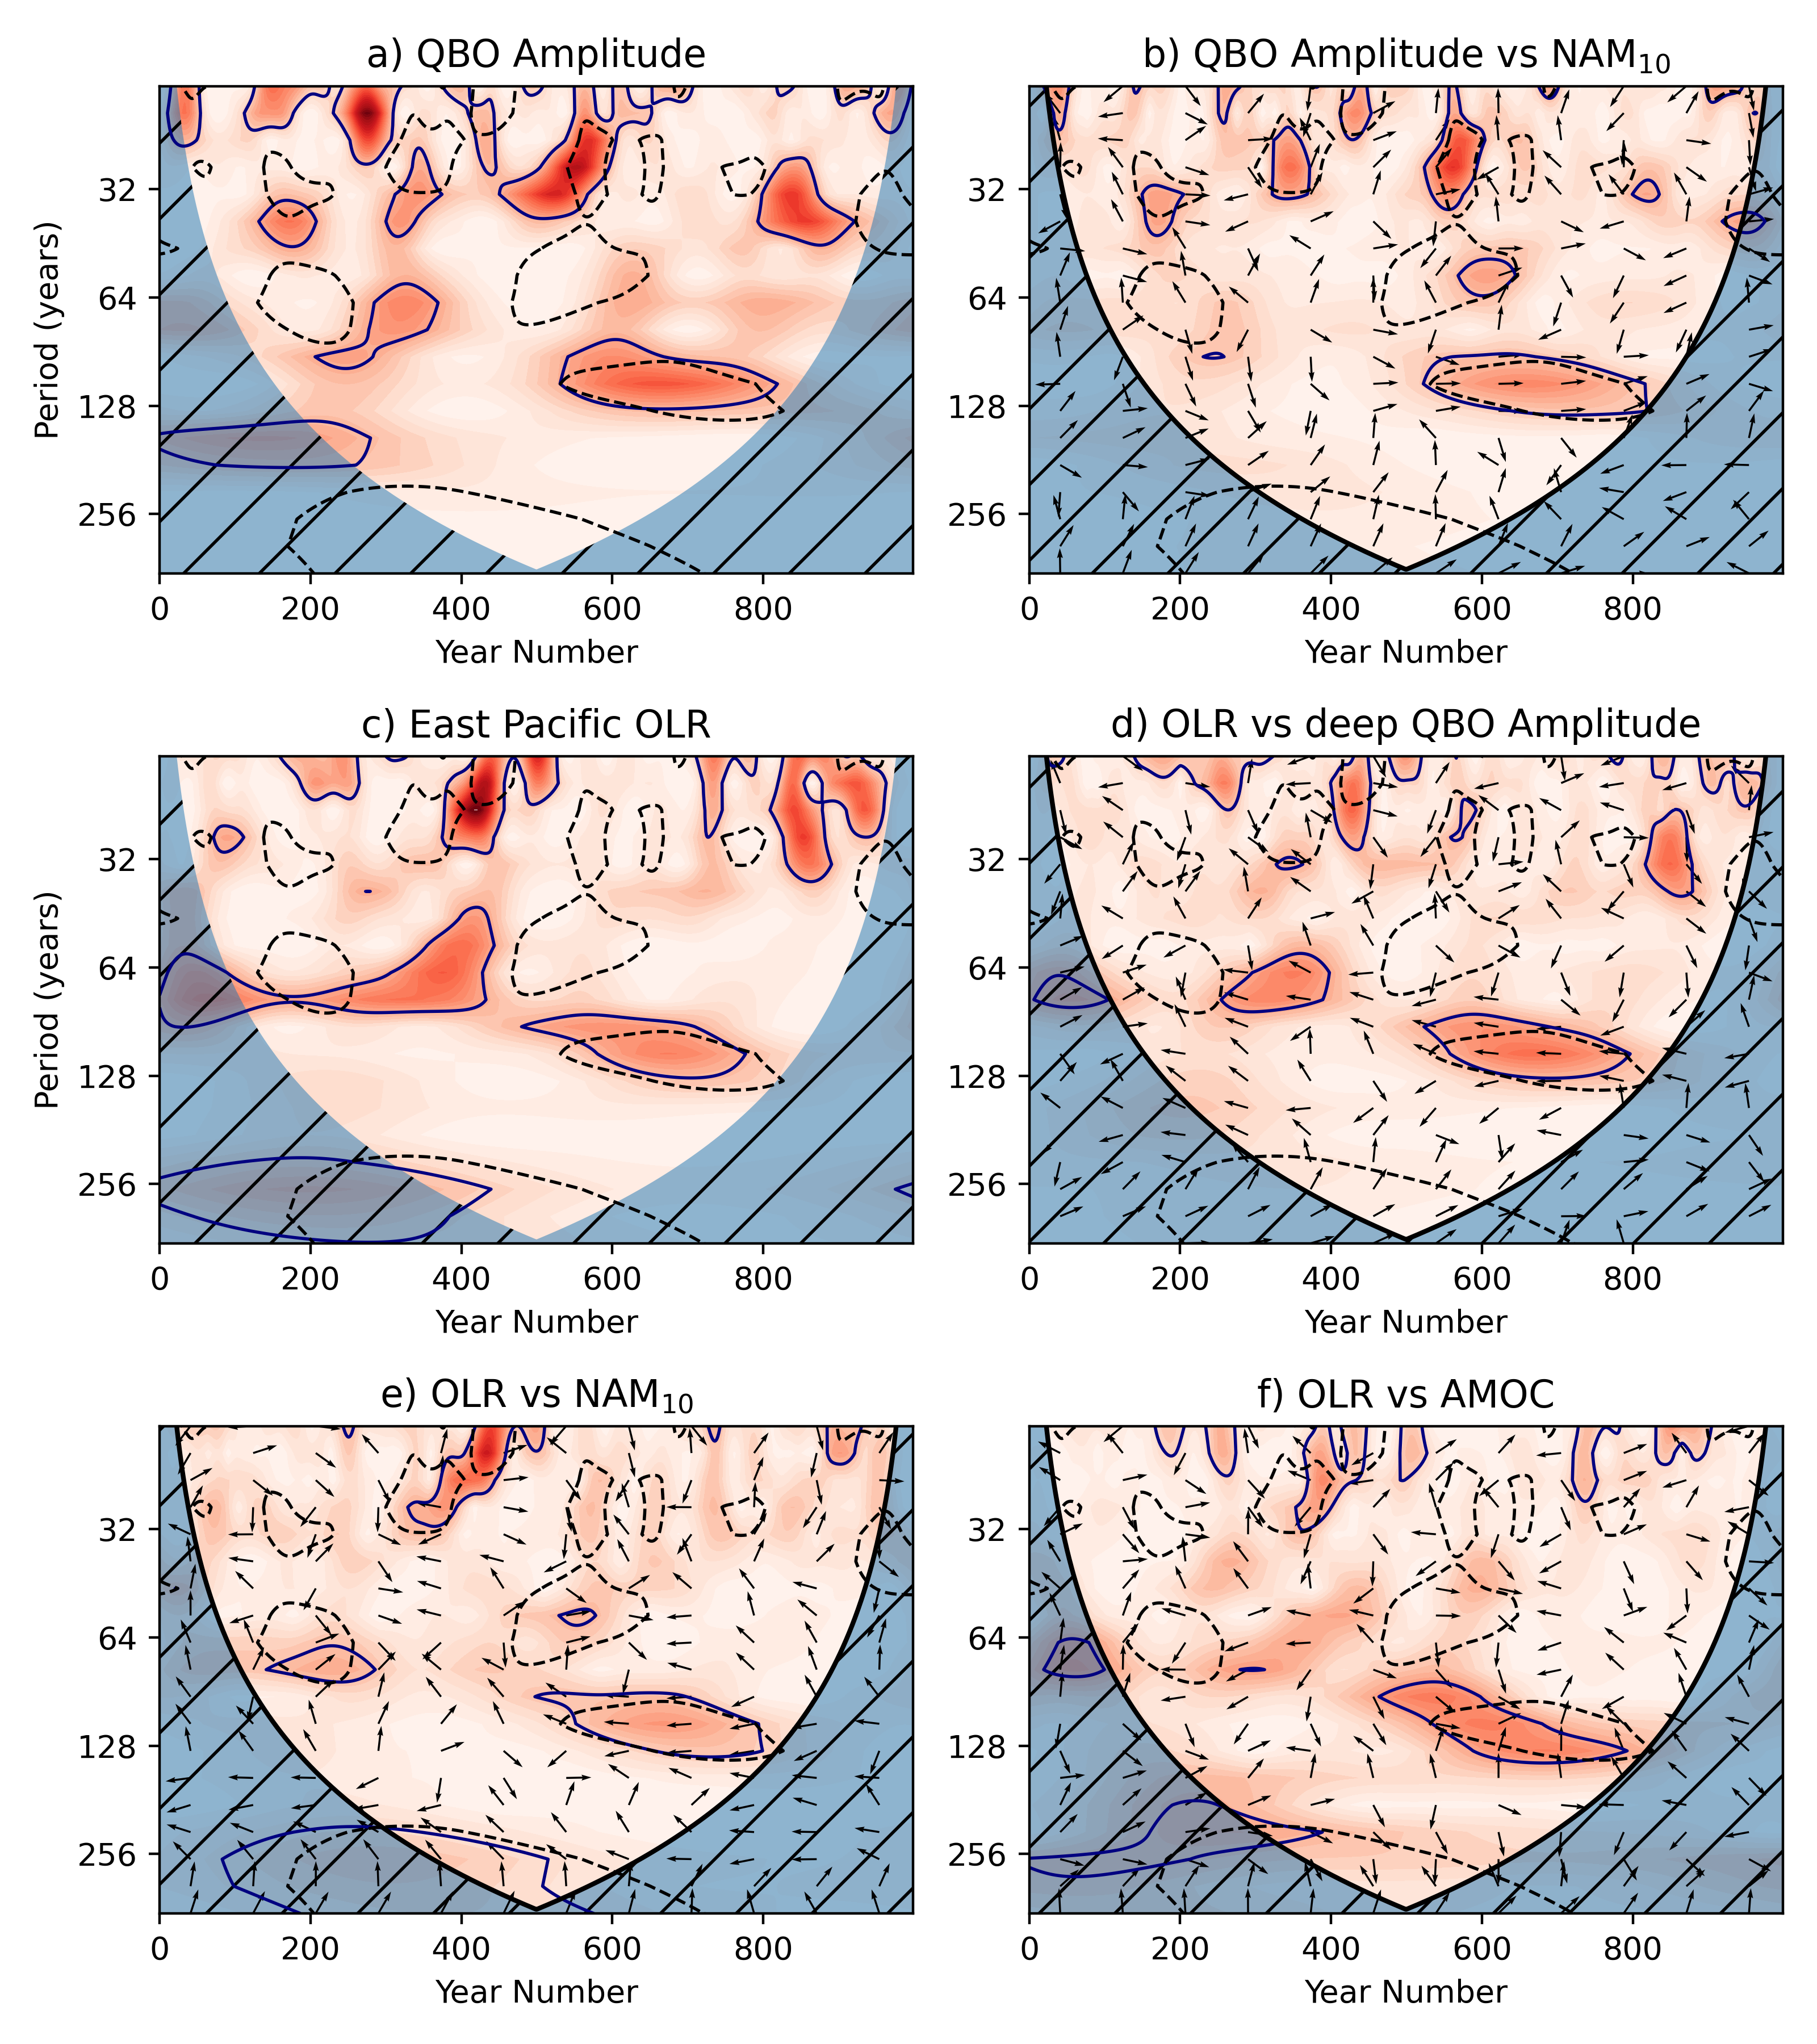
\includegraphics[width = 0.7\linewidth]{Figures/Figures-surface/OLR_wavelet.png}
\caption{\textbf(a): Wavelet power spectrum for the Sep-Nov deep QBO amplitude (see section \ref{sec:model_diagnostics_surface}). \textbf(b) cross power spectra between deep QBO Amplitude (Sep-Nov) and smoothed NAM$_{10}$ (Dec-Mar). \textbf(c): Wavelet power spectrum for the Sep-Nov  Area weighted average equatorial East Pacific OLR (see section \ref{sec:model_diagnostics_surface}). \textbf{d-f}: cross power spectra between combinations of East Pacific OLR, deep QBO Amplitude (both Sep-Nov means), AMOC at 50N (annual mean, all months) and NAM$_{10}$ (Dec-Mar) indices all smoothed with the same Gaussian filter as is used throughout ($\sigma$ = 2 years). Indices involved are indicated by sub-figure titles, shading indicates cross power with a colour scale the same as that seen in figures 6-8, dashed contours the 95\% confidence interval for the NAM$_{10}$ spectrum and arrows the relative phase angle between signals in the indices.}
\label{OLR_wavelet}
\end{center}
\end{figure}


\section{Contribution of the stratosphere to recent AMOC changes}
\label{sec:AMOC_obs_contribution}
Our analysis of the UKESM simulation has identified co-variations between modes of variability in stratospheric circulation and the AMOC. Intervals in which the winter stratospheric polar vortex is consistently strong are, on average, followed by an extended negative anomaly in AMOC strength with a lag of approximately 15-20 years (figure \ref{AMOC_comp_NAM}f). Recent observations of the AMOC have shown a negative trend in circulation strength of approximately $-2.7 Sv$ between 2004 and 2012 \citep{smeedNorth2018} before a marginal recovery after 2012 \citep{smeedAtlantic2019}. Modelling studies have proposed a key role for anthropogenic forcing in AMOC slowdown over the 20th century and into the future \cite{liuOverlooked2017, bakkerFate2016, liuMechanisms2019} however, the magnitude of this contribution as well as others carries significant uncertainties. Furthermore, the results shown in the previous sections suggest the possibility that stratospheric variability has also contributed to the observed AMOC changes, in response to nearly a decade of strong vortex years in the 1990s followed by a sequence of years with a weak, disturbed vortex in the early 2000s \citep{pawsonCold1999, manneyRemarkable2005}. 

To assess the potential role of stratospheric variability figure \ref{ERA5_series} shows the NAM, AMOC and NAO indices for the interval 1979-2020 from the ERA5 and rapid array datasets. The NAM$_{10}$ index is characterised by an interval of strong vortex winters between 1988 and 1997 in which all but 2 winters exhibited a positive NAM$_{10}$. This interval also contains no SSWs \citep{pawsonCold1999}. This is followed by a run of winters between 1998 and 2005 which exhibit anomalously weak NAM$_{10}$ values \cite{manneyRemarkable2005}. The filtered NAM$_{10}$ index (red dashed line) reflects the presence of these intervals with a peak in positive values centred around 1995 followed by a negative extreme centred around 2003. The smoothed NAO (green dashed line) from the same dataset broadly reflects these variations in the NAM$_{10}$ with positive NAO extremes in the 1990s. The long-term envelope of the NAO does not remain positive for as long as the NAM, primarily due to the anomalous negative NAO in 1996 \citep{halpertClimate1997}. The presence of this anomalous negative NAO in 1996 and the absence of a clear NAO anomaly in the following year despite the presence of strong positive anomalies in the stratospheric NAM$_{10}$ is indicative of the fact that there are many other factors that influence the NAO in addition to the stratospheric influence. The AMOC strength at 26N estimated from the Rapid Array observations between 2005 and 2019 are also shown (blue curve) and shows a negative trend between 2005 and 2012 followed by a recovery from 2012 onwards consistent with \cite{smeedNorth2018} and \cite{smeedAtlantic2019}. 

\begin{figure}[h!]
\begin{center}
\noindent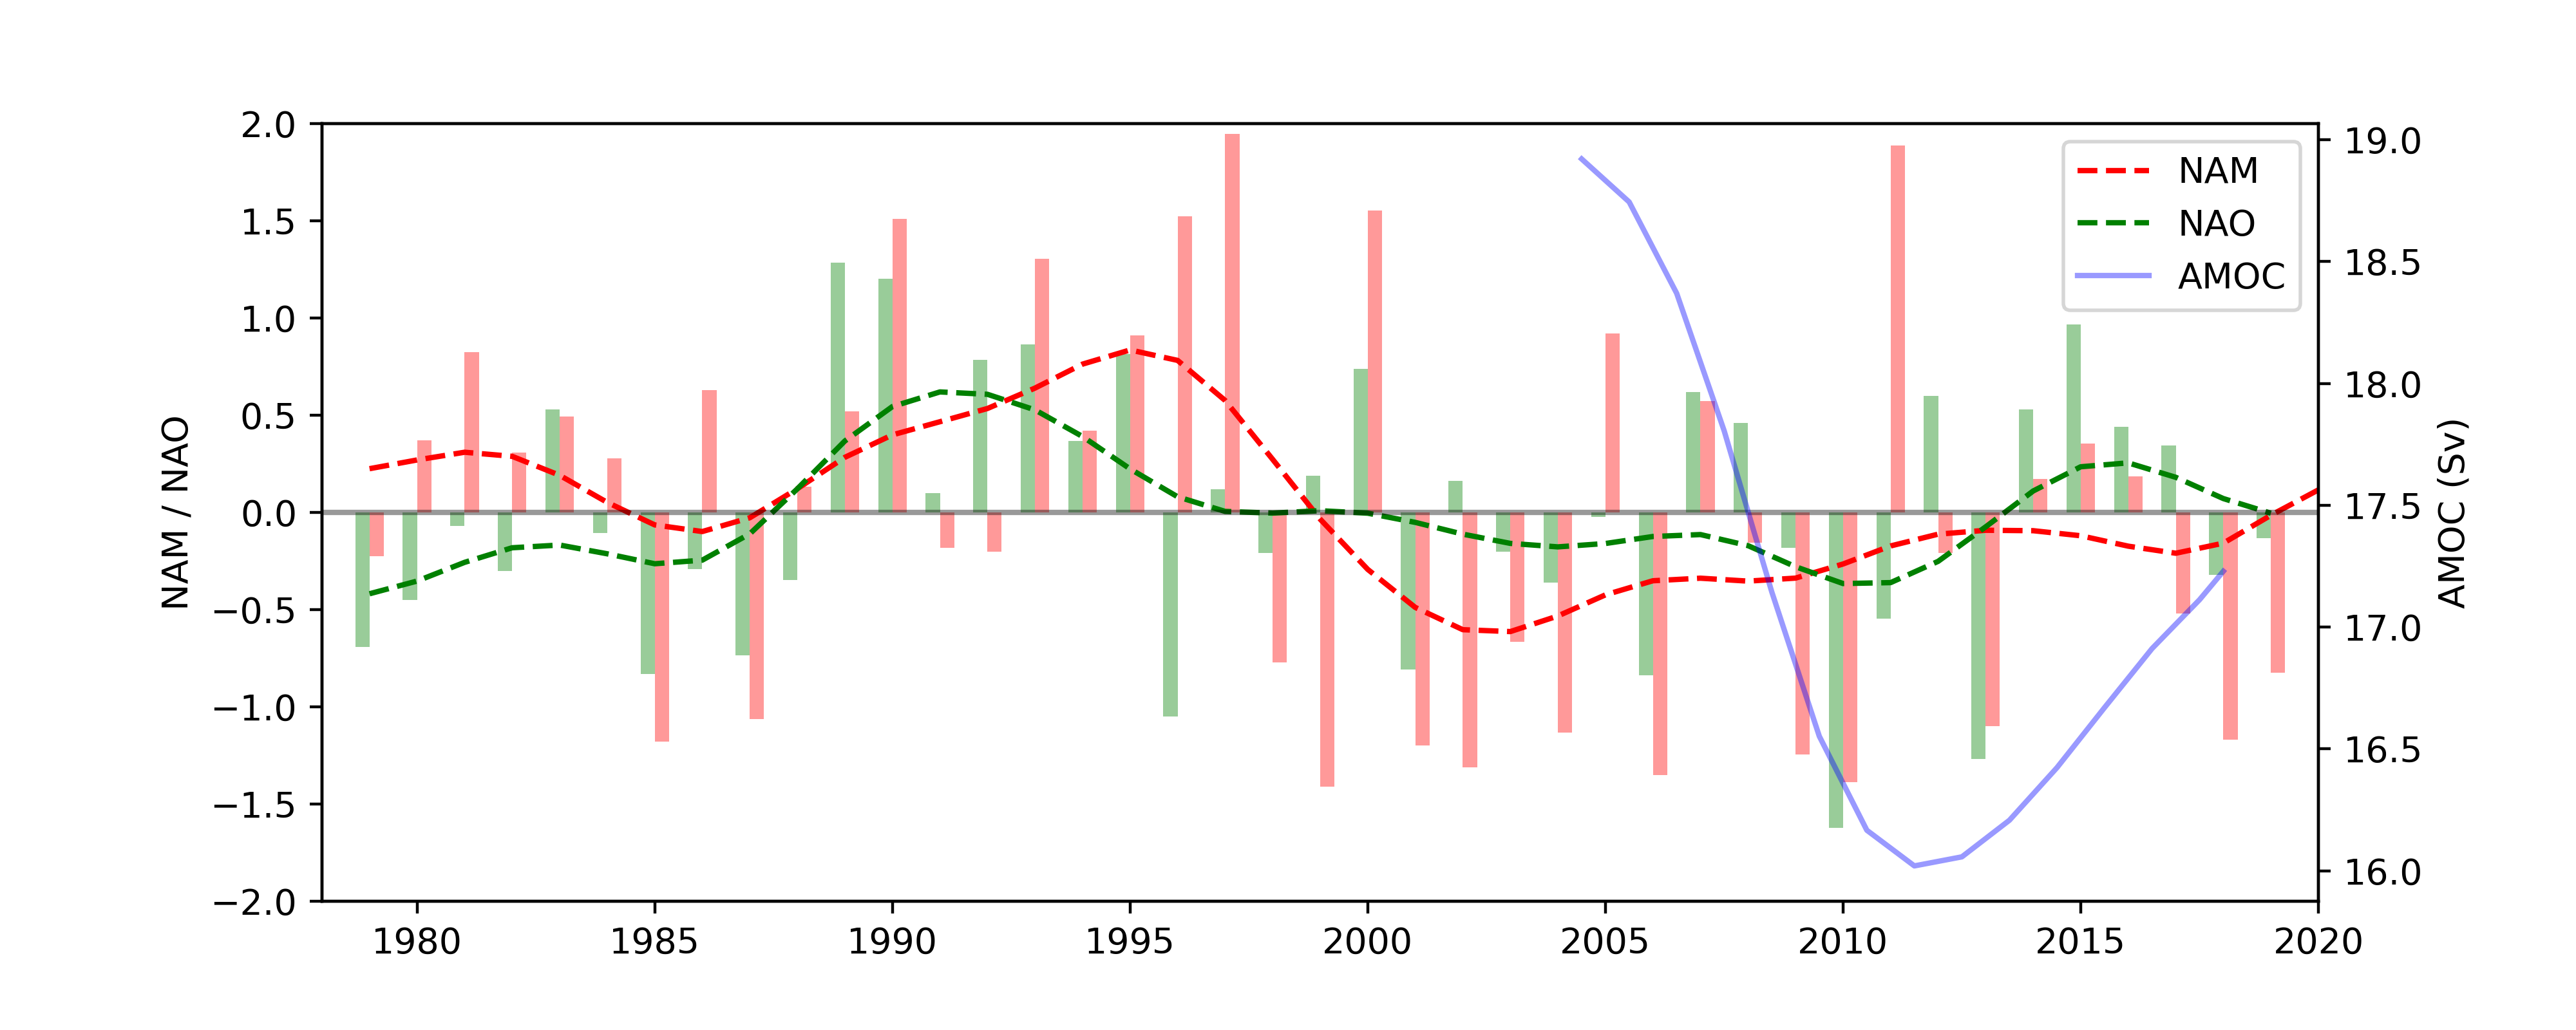
\includegraphics[width = 0.9\linewidth]{Figures/Figures-surface/ERA5_series_allf.png} \caption{Time series of the Dec-Mar NAO index (green bars), NAM$_{10}$ index (red bars) from the ERA5 dataset. Dashed lines correspond to indices shown by bars smoothed with a Gaussian filter ($\sigma$ = 2 years). Also included is the  AMOC timeseries at 26N from the rapid array dataset (blue) also smoothed with the same filter.}
\label{ERA5_series}
\end{center}
\end{figure}

The interval of observed consecutive strong NAM winters in the 1990s is anomalous in the reanalysis period although the available data record is rather short to allow a robust assessment. The amplitude and longevity of the observed anomaly is also large when compared to the UKESM simulation. Only 2 intervals in the simulation exhibit at least as many consecutive winters with strong (high NAM$_{10}$) conditions. These 2 intervals occur in the 300-400 year interval (centred around years 349 and 376) as shown in figure \ref{special_events}a. they exhibit a sequence of 10 and 14 consecutive Dec-Mar anomalously positive NAM$_{10}$ values respectively. This is reflected in the smoothed NAM$_{10}$ values (figure \ref{special_events}b) and these intervals represent the two of the three largest values of the filtered NAM$_{10}$ index (0.66 and 0.67). The corresponding smoothed AMOC index during these 2 intervals (blue curve in figure \ref{special_events}b) shows a positive AMOC response at lags of 2-3 years followed by a negative response at 17-20 years, in good agreement with figure \ref{AMOC_comp_NAM}f. The negative responses at 17-20 years following these 2 intervals of strong NAM$_{10}$ years are the 1st and 3rd greatest in magnitude compared to all other responses to persistent strong intervals. This is confirmed by figure 11b which shows the lagged AMOC response following all of the identified intervals with persistent positive NAM$_{10}$ anomalies (the two identified around 349 and 376 years are shown in black). 

To estimate the response amplitude of the AMOC to an interval of persistently strong vortex years figure \ref{special_events}d shows a scatter plot of the NAM$_{10}$ index evaluated at the centre of these intervals against the AMOC anomaly at 50N lagged by 17 years. This reveals a strong linear relationship ($r = -0.908$) between the size of the persistent vortex anomaly and the subsequent negative anomaly in the AMOC at 50N 17 years later. This correlation appears large and may indicate a strong relationship between stratospheric extreme and subsequent AMOC anomaly. However, given the relatively few anomalous vortex intervals selected (top 5 percentiles of the smoothed NAM$_{10}$) we must consider the probability that this correlation appears even if the lagged response in the timeseries occurs by chance. To assess this probability, we estimate a significance level for this value of $r = -0.908$ by assessing the probability such a value results if the phases in signals in the NAM$_{10}$ and AMOC are randomly assigned but the overall autocorrelation structure of each time-series is retained. We compare the $r$ value stated above with those produced from a set of synthetic NAM$_{10}$ series. These synthetic data are generated by Fourier transforming the smoothed NAM$_{10}$, randomly shuffling the Fourier phases and subsequently inverse Fourier transforming to generate a surrogate timeseries with the same Fourier power spectrum as the real data. Repeating this data generation and calculating the correlation between the magnitude of positive extremes in the surrogate NAM$_{10}$s and the 17 year lagged AMOC builds up a PDF for the $r$ value. This PDF of correlations is displayed in figure \ref{cors_stat_sigs}a (blue bars) along with the correlation generated by the real NAM$_{10}$ data (black vertical line). It shows that the $r$ value lies well outside the distribution of surrogate correlations indicating the high level of significance of the linear relationship.

A linear regression analysis on this data yields an estimated relationship between the variables which satisfies

\begin{equation}
AMOC'_{+17} = -6.54\space NAM max + 3.11,
\end{equation}

where $AMOC'_{+17}$ is the 17 year lagged AMOC anomaly at 50N and $NAM max$ is the magnitude of the positive extreme in smoothed NAM$_{10}$ at the centre of each interval. We can then use this relationship to predict the AMOC response to the observed sequence of strong vortex years in the 1990s. The maximum smoothed NAM$_{10}$ occurs in 1996 so the maximum AMOC response associated with the stratosphere would be 17 years later (2013) with amplitude of -0.89 Sv (figure \ref{special_events}d, purple point). This prediction suggests that $\sim$30\% percent of the observed reduction in AMOC strength  between 2005 and 2013 (0.89 Sv compared with 2.9 Sv in total) could be due to the presence of the persistent strong vortex winters that occurred during the 1990s. However, we acknowledge that the comparison between the interactions between the stratosphere and the AMOC at 50N in the model and 26N in observations may not be direct. Indeed, the modulation of the AMOC by the smoothed NAM$_{10}$ is less pronounced at 30N (figure \ref{AMOC_comp_NAM} and b) that at higher latitudes. Nevertheless, the Rapid Array dataset remains the most direct measurement of AMOC strength over the last 15 years and results from UKESM suggest a possible significant contribution towards trends over early the 21st century.  A similar analysis of the relationship between the magnitude of smoothed negative (weak) NAM$_{10}$ extremes and the lagged AMOC response (not shown) yields a significantly weaker relationship ($r = -0.21$). A similar significance analysis using surrogate time-series (see paragraph above) is shown in figure \ref{cors_stat_sigs}b, it shows that this $r$ value lies well within the PDF of surrogates suggesting the relationship may not be robust. This asymmetry in the relationship between extreme types is likely due to differences in dynamical behaviour associated with each extreme outlined in section \ref{persistent}. Namely that the surface signature of weak anomalies associated with SSWs are highly dependant on the timing of the SSW within the winter season while strong intervals generally exhibit strong vortex conditions throughout a winter.  

\begin{figure}[h!]
\begin{center}
\noindent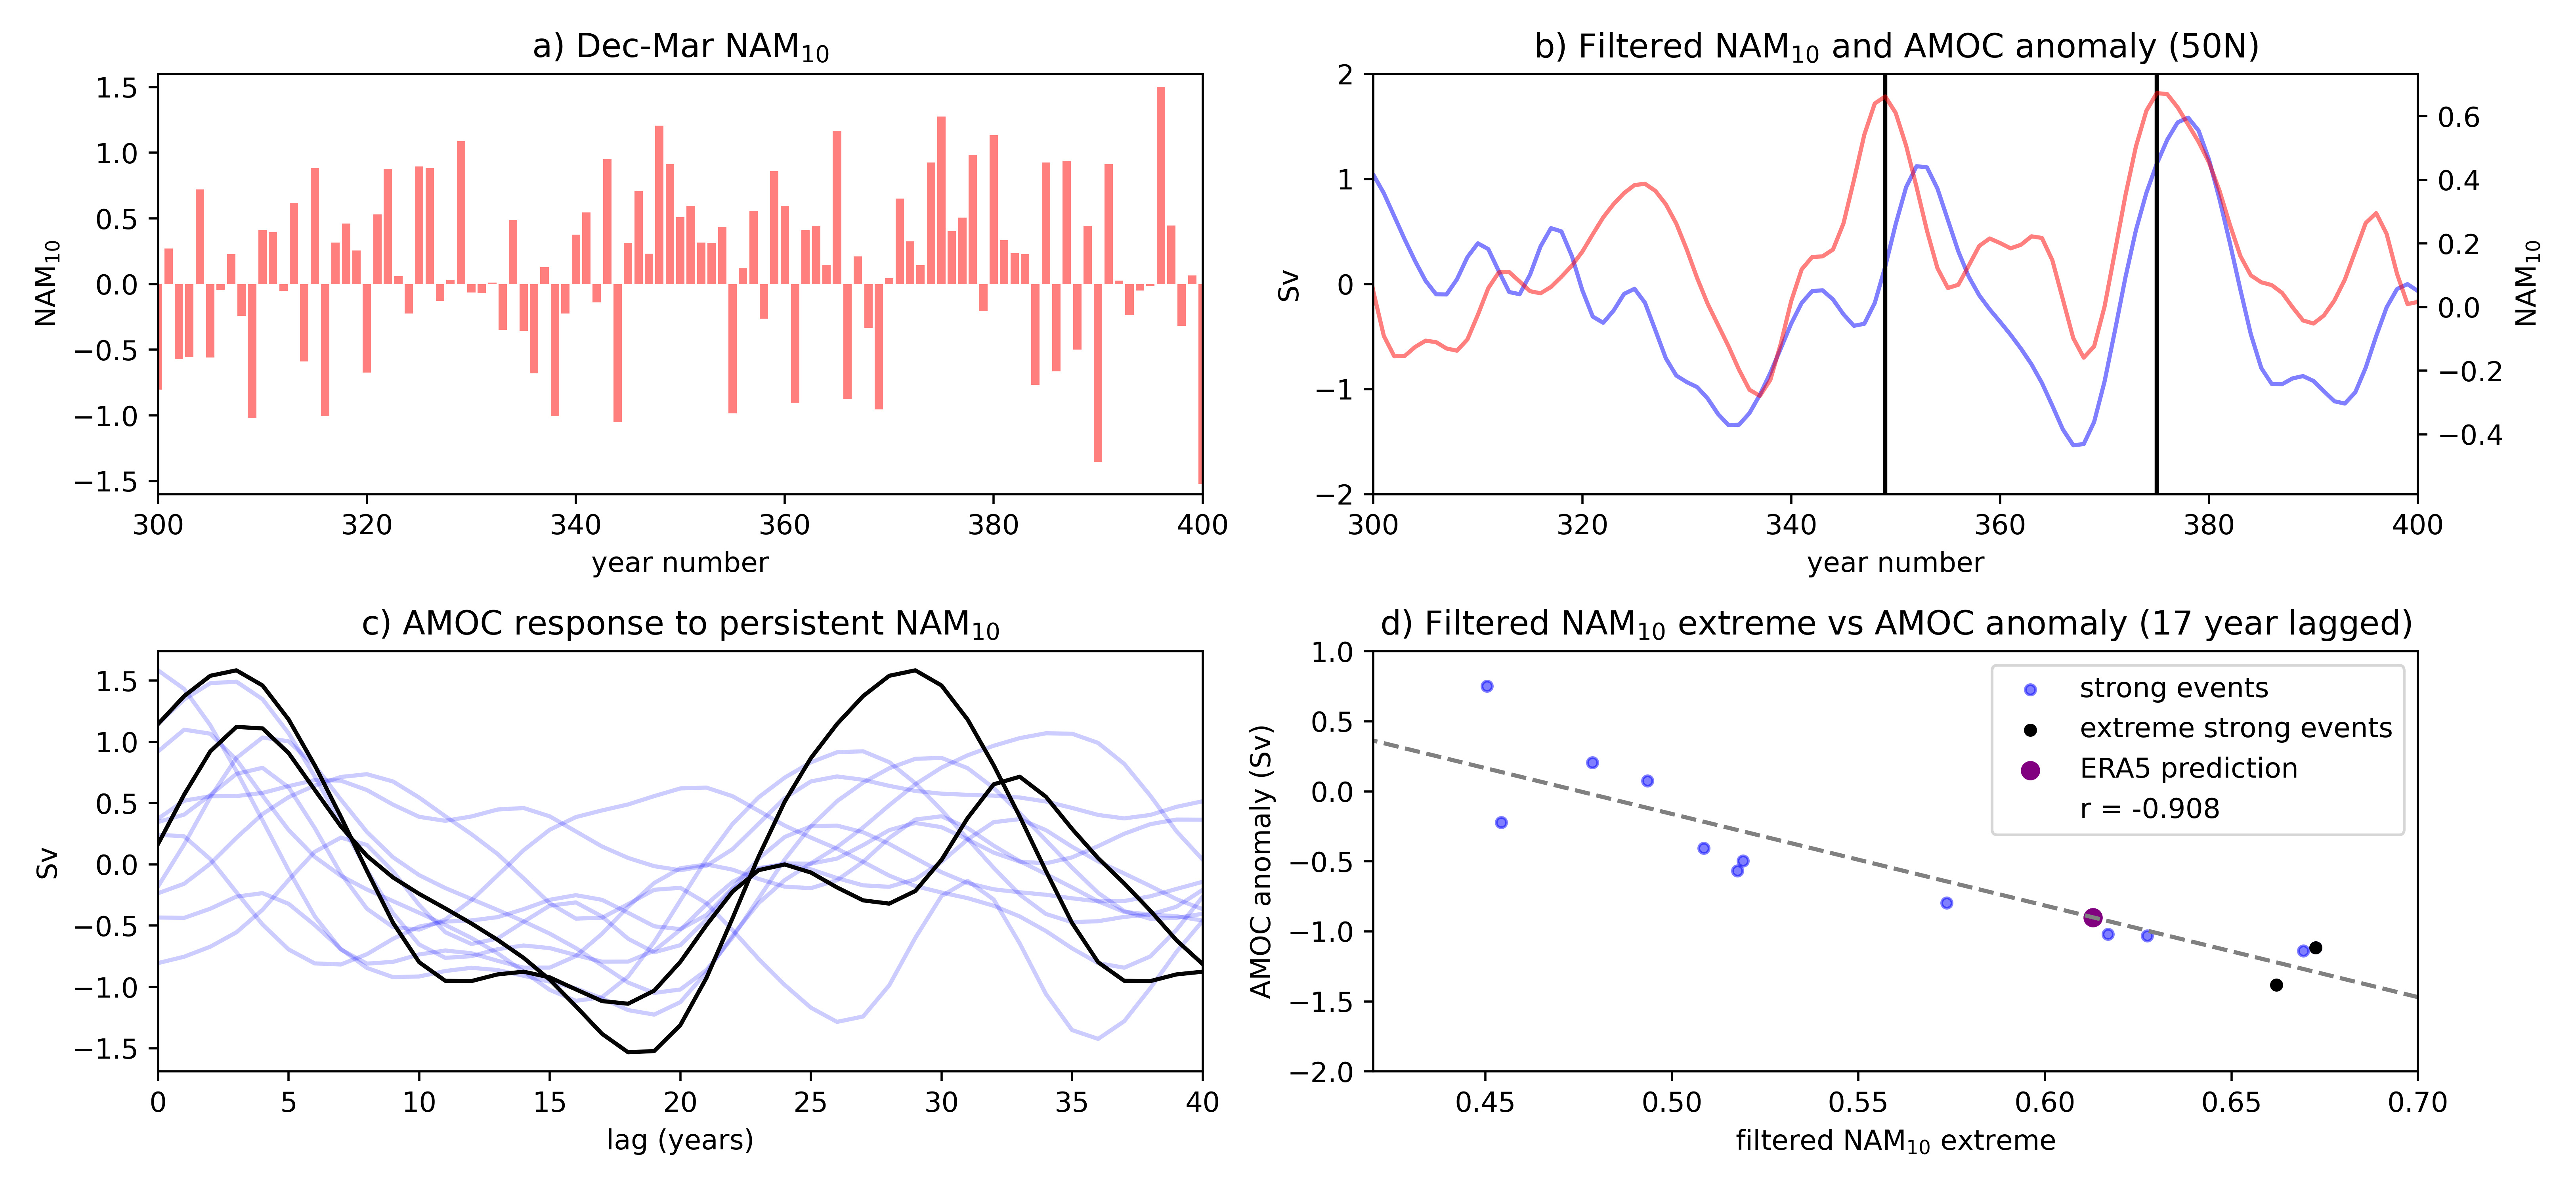
\includegraphics[width =\linewidth]{Figures/Figures-surface/AMOC_response_special_events.png} 
\caption{\textbf{a}: AMOC (blue) and NAM$_{10}$ (red) indices smoothed with the Gaussian filter ($\sigma$ = 2 years) between year numbers 300 and 400 of the UKESM simulation. \textbf{b}: AMOC at 50N associated with persistent strong NAM$_{10}$ intervals (light blue) and the intervals marked in \textbf{a} (black). \textbf{c}: Dec-Mar NAM$_{10}$ index from the UKESM simulation between year numbers 300 and 400. \textbf{d}: Scatter plot of filtered NAM$_{10}$ index values occurring at persistent strong NAM$_{10}$ intervals ($y$ axis) against AMOC anomalies at 50N lagged 17 years after persistent intervals' central year ($x$ axis). Blue points indicate persistent intervals and black dots represent the 2 intervals in the interval displayed in a. The dotted line represents the linear line of best fit for the points in black and blue. Also included is the 17 year lag AMOC anomaly predicted by projecting the regression coefficients used to construct the linear fit onto the maximum smoothed NAM$_{10}$ index in the ERA5 dataset (purple point).}
\label{special_events}
\end{center}
\end{figure}

\begin{center}
\begin{figure}[h!]
\noindent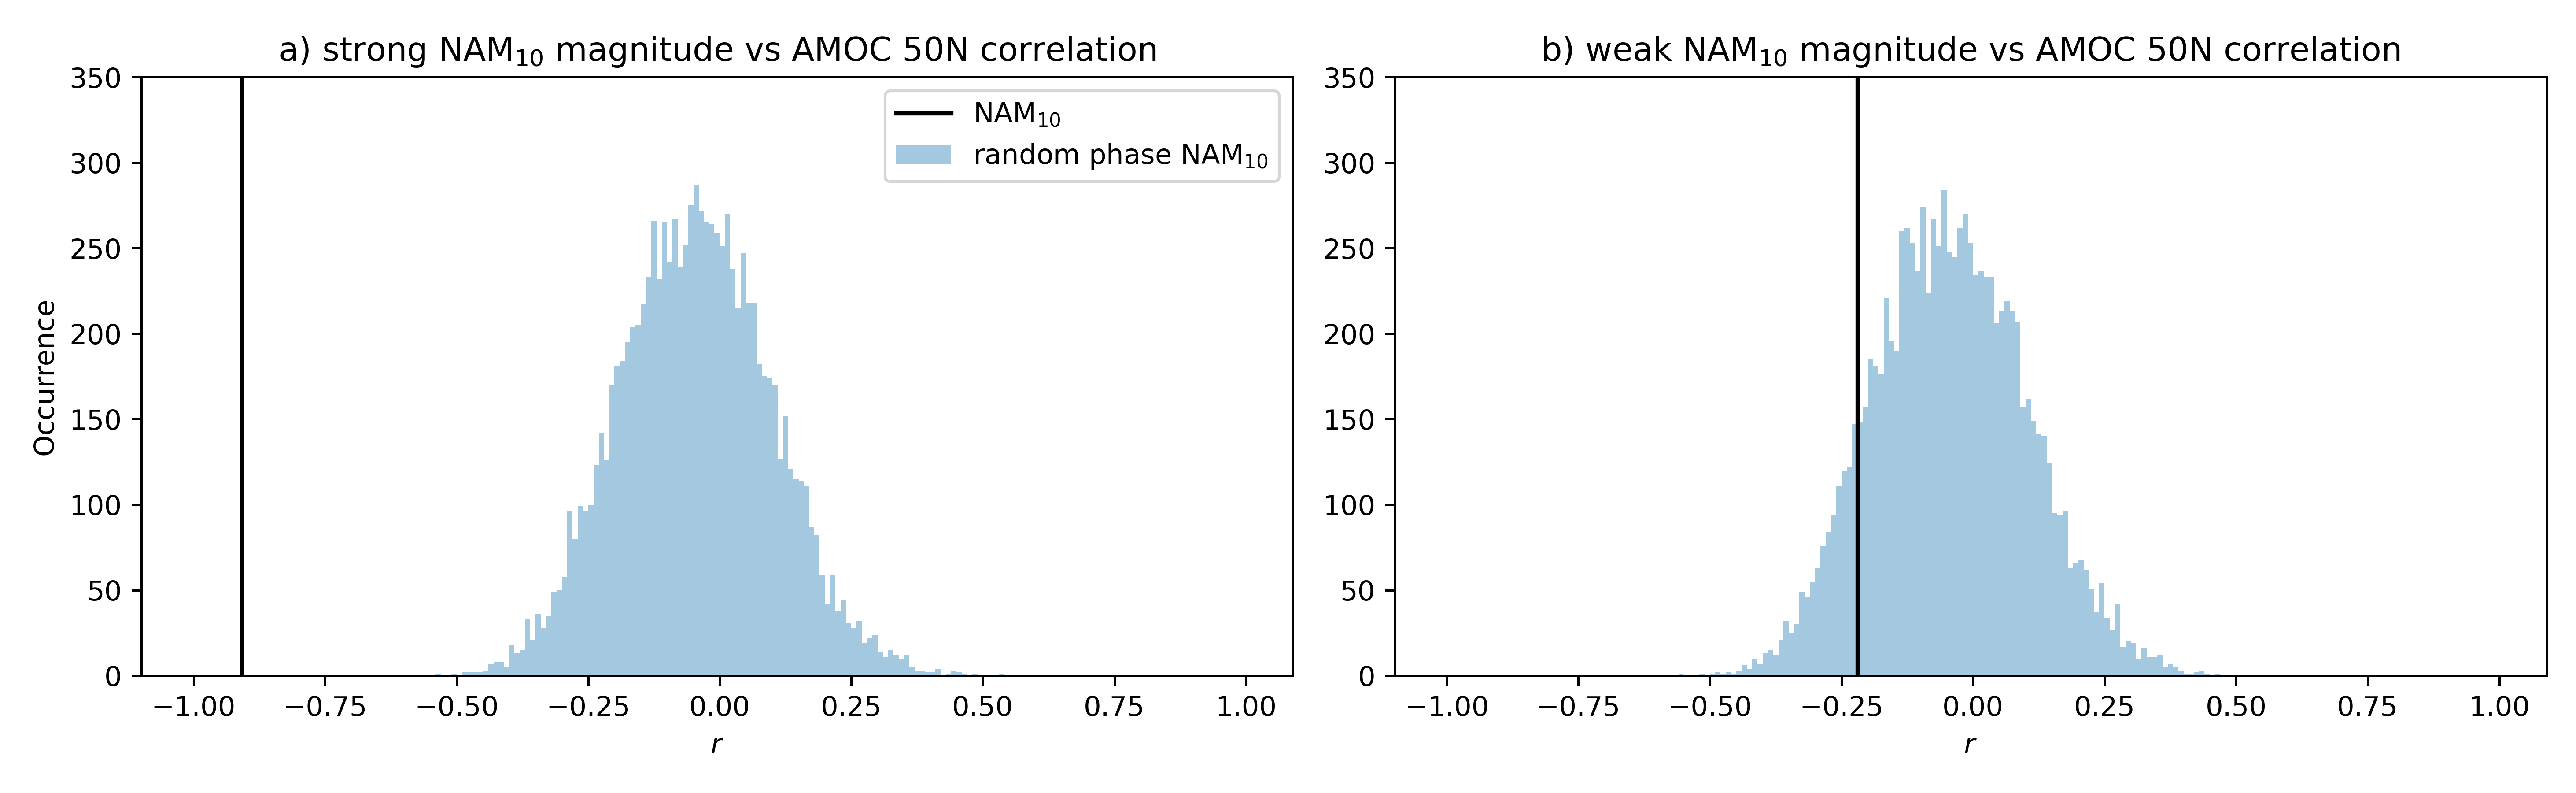
\includegraphics[width = \linewidth]{Figures/Figures-surface/correlation_stat_sigs.png}
\caption{Probability distribution functions (PDFs) for correlations between the magnitude of NAM$_{10}$ extreme positive (\textbf{a}) and negative (\textbf{b}) values from surrogate NAM$_{10}$ data and anomalies in the AMOC at 50N evaluated 17 years later. Each NAM$_{10}$ surrogate is generated by Fourier transforming the smoothed NAM$_{10}$ index, randomly shuffling the Fourier phases and inverse transforming. Each PDF is built with 10000 surrogates and the correlation between the NAM$_{10}$ extreme magnitude and 17 year lagged AMOC anomaly at 50N is shown by vertical black lines in both subfigures.}
\label{cors_stat_sigs}
\end{figure}
\end{center}

\section{Sensitivity to NAM thresholds and filtering}

The results showing interactions between the vortex and the AMOC presented so far (figures \ref{AMOC_comp_NAM} and \ref{NAO_AMOC_T_response}) are derived from a stratospheric index which is highly processed. The NAM$_{10}$ is both smoothed using a Gaussian filter and extreme values are subsequently selected to define intervals of anomalous vortex behaviour. Lagged responses of the AMOC are then obtained from these intervals. This processing relies on a number of parameters that need to be chosen: First, the filtering kernel width (the parameter $\sigma$, see equation \ref{Gaussian_filter}) which dictates the number of years which contribute to smoothed NAM$_{10}$ values. Second, the threshold value of the smoothed NAM$_{10}$ used to define an interval of persistent vortex behaviour. Finally, for regression analysis such as that presented in figure \ref{special_events}d, the lag of the AMOC response in years used to correlate the magnitude of NAM$_{10}$ extreme with the resulting AMOC anomaly. 

So far, we have chosen these parameters in line with previous studies that utilise a similar smoothed NAM$_{10}$ metric \citep{reichlerStratospheric2012}. Namely, we utilise $\sigma$ = 2 years to smooth all indices which allows contributions from approximately 6 years either side of the interval centre which is approximately the length of the interval of persistent strong vortex behaviour in the 1990s of ERA5 (see figure \ref{ERA5_series}). We also utilise 5th and 95th percentiles to define weak and strong extremes respectively in the smoothed NAM$_{10}$. This yields approximately the same average rate of persistent vortex intervals in the pi-cntrl of UKESM as appears in the modelling study of \cite{reichlerStratospheric2012}. While values of these parameters may dictate some key physical features of the timeseries (for example interval width in years), there is little obvious justification for parameter choices. In this section, we test the sensitivity of our results on vortex-AMOC interactions on choice of smoothing width ($\sigma$), NAM$_{10}$ threshold and AMOC lag values. 

First, we assess the impact of parameter choice on lagged response values of the AMOC at 50N, the latitude at which the most prominent interactions were shown (see figure \ref{AMOC_comp_NAM}, following persistent NAM$_{10}$ extremes (figure \ref{sensitivity}). Parameter grids of the response to strong intervals for different combinations of lag and $\sigma$ (figure \ref{sensitivity}a) show a similar response variation with lag as that shown in figure \ref{NAO_AMOC_response_individual_types} - positive responses peaking 2-3 years following stratospheric extremes followed by negative responses at 10-20 year lags. However, the largest negative response magnitude is observed when the NAM$_{10}$ index is smoothed using $\sigma = \sim 5 years$ at a lag of approximately 15 years instead of our original choice of $\sigma$ = 2 years lagged by 17 years (as was used in figure \ref{special_events}d). This suggests that the AMOC responds most prominently to intervals which consist of contributions from approximately 10-15 years either side of the the central year. Extremes intervals of this size are unlikely to consist of winters exhibiting all the same sign of vortex anomaly due to their length - the largest run of consecutive positive NAM$_{10}$ winters are shown in figure \ref{special_events} and are only 10 and 12 years respectively. Instead, these are likely intervals containing a combination of elevated NAM$_{10}$ and neutral (near 0 smoothed NAM$_{10}$) winters - I.E. intervals that consist of winters with either a strong vortex or one that exhibits near climatological vortex winds and even those that may feature partial minor disruptions. This suggests that a key factor in the AMOC response to the vortex may not simply be the presence of $\sim 6-8$ consecutive strong vortex seasons for but the absence of major SSWs over a longer interval ($\sim$10-15 years). While this result indicates a larger response using a wider smoothing window, applying this to observations like the analysis in section \ref{sec:AMOC_obs_contribution} may be difficult given the width of the window (including contributions from 10-15 years either side of the centre) in relation to the length of the observational record (approximately 40 years in ERA5). Furthermore the observational record does not exhibit such a large interval of persistent vortex behaviour and the most prominent feature of the ERA5 NAM$_{10}$ is the interval of approximately 8 years of strong NAM$_{10}$ winters in the 1990s which is well captured using $\sigma$ = 2 years. 

The AMOC response magnitude is also sensitive to varying the percentile threshold used to define persistent vortex intervals. Figures \ref{sensitivity}b and c show the variation in response for different combinations of threshold and $\sigma$ and threshold and lag. Both sub-figures indicate that the average AMOC response magnitude increases significantly with threshold percentile over values of approximately 95\%. This increase in magnitude is expected as increasing the threshold for events will include NAM$_{10}$ intervals which on average contain more years with an anomalously strong vortex and likely a more persistent source of atmospheric forcing to the NAO and the ocean. 


\begin{figure}[h!]
\begin{center}
\noindent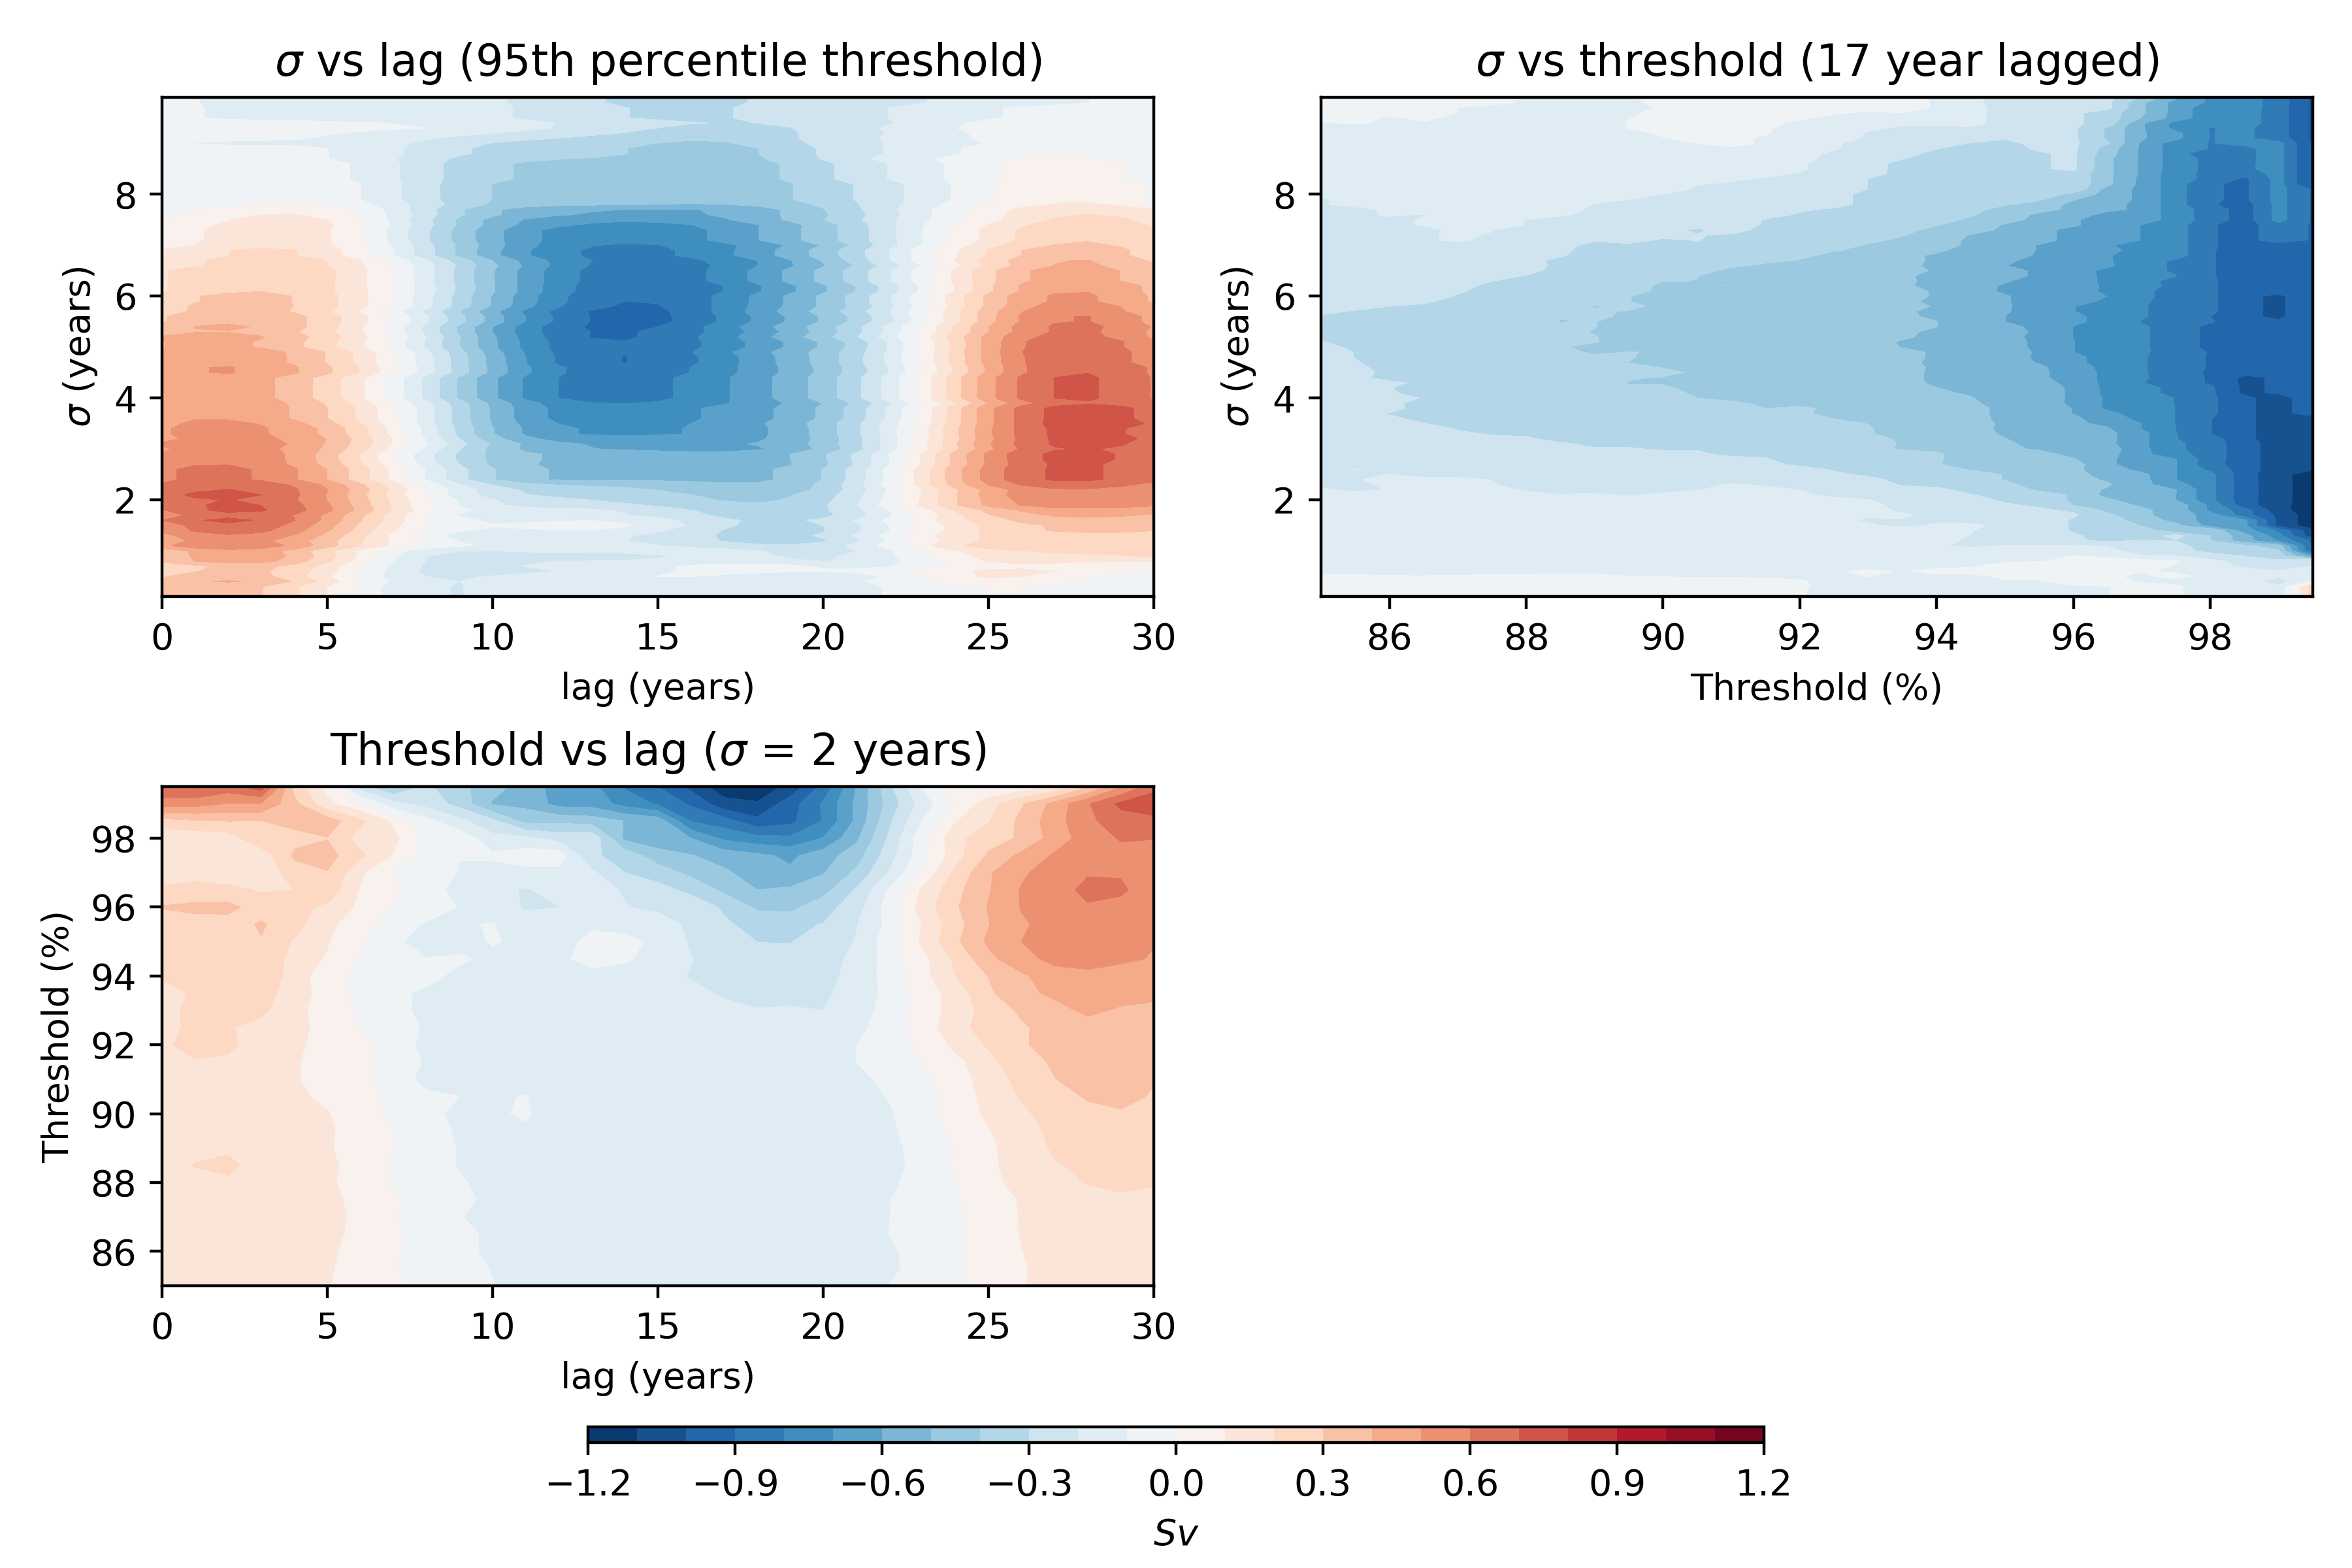
\includegraphics[width =\linewidth]{Figures/Figures-surface/sensitivity_contours_strong.png} 
\caption{Response of the AMOC at 50N to strong NAM$_{10}$ intervals for combinations of \textbf{a):} smoothing width ($\sigma$) and lag both measured in years with percentile threshold held at 95\%, \textbf{b):} $\sigma$ and percentile threshold used to define persistent NAM$_{10}$ extremes with a 17 year lag and \textbf{c):} Threshold and lag with $\sigma$ = 2 years.}
\label{sensitivity}
\end{center}
\end{figure}

We also test the sensitivity of our key result outlined in section \ref{sec:AMOC_obs_contribution}, that the magnitude of NAM$_{10}$ extremes is directly proportional to the AMOC anomaly 17 years later, to parameter choices. Figure \ref{cors_stats_parameters_strong} shows the correlation between strong NAM$_{10}$ extremes and the lagged AMOC anomaly at 50N (black vertical lines) for a range of threshold percentile values used to define persistent vortex intervals (increasing in panels left to right) and smoothing widths ($\sigma$, increasing top to bottom). Each correlation's significance level is compared to a PDF of surrogate correlations constructed using the same procedure as described for figure \ref{cors_stat_sigs}. For values of $\sigma$ between 2 and 7 years, the real correlation lies on the edge of the surrogate correlation PDF for all values of threshold percentile. This suggests the relationship between positive extremes in the smoothed NAM$_{10}$ and the resulting AMOC response is robust to the definition of strong persistent vortex interval for these values of smoothing width. for $\sigma$ = 1 year, the correlation lies well within the distribution surrogate PDF for all sampled values of threshold percentile suggesting the vortex-AMOC interaction is significantly weakened for these parameter combinations. This weakening is accounted for by the fact that with a filtering kernel with $\sigma$ = 1 year, contributions from only approximately 3 years either side of the interval centre (with the majority of contributions from 1-2 years either side) are included in smoothed NAM$_{10}$ values. This may not be sufficient to provide atmospheric forcing persistent enough to induce significant correlations between NAM$_{10}$ extremes and AMOC anomalies. For $\sigma$ values larger than 7 years, the correlations are also deemed not significant against the bootstrapping test for the sampled values of percentile thresholds. This is because at such large values of $\sigma$, each index is smoothed over time intervals as larger or larger than the lags considered in this analysis (17 years). As a result, variations in the NAM$_{10}$ and AMOC on timescales up to and beyond 17 years are removed thus also removing significant correlations.

\newpage
\begin{landscape}
\begin{figure}[h!]
\begin{center}
\noindent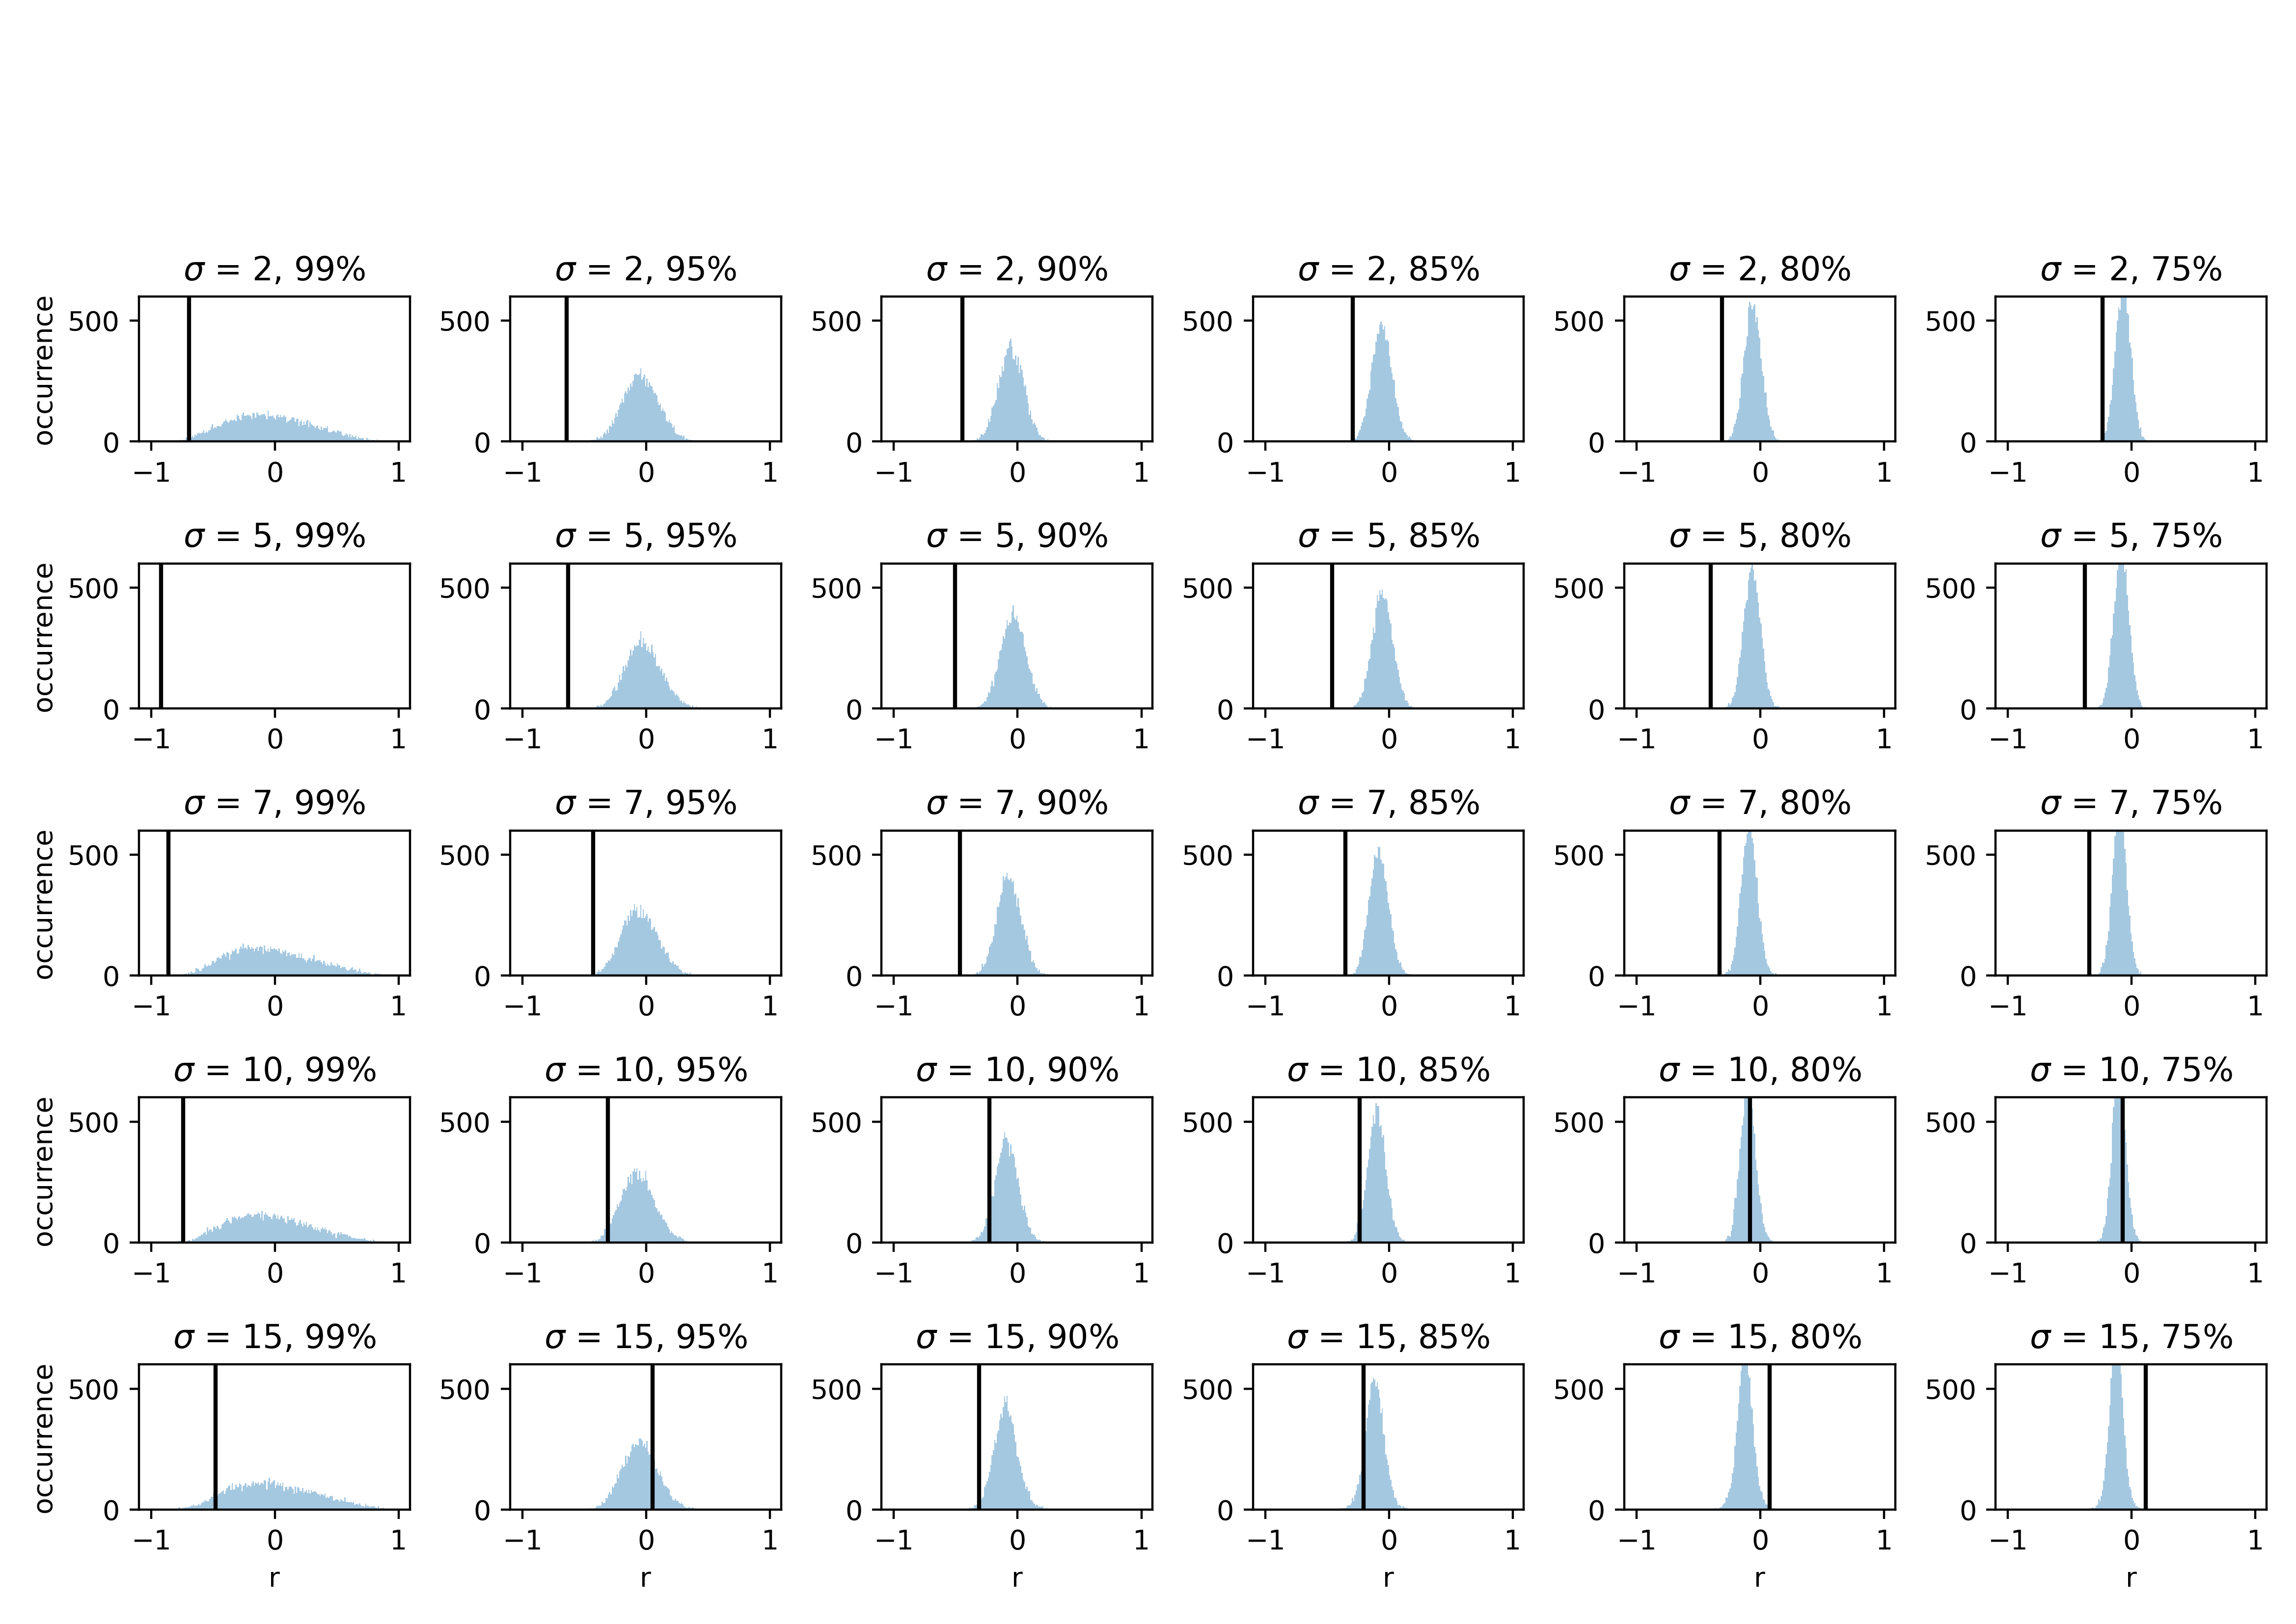
\includegraphics[width =0.9\linewidth]{Figures/Figures-surface/cors_sigs_thresh_and_sigma.png} 
\caption{like figure \ref{cors_stat_sigs}a for different combinations of smoothing width ($\sigma$) (increasing in panels top to bottom) and percentile used to define NAM$_{10}$ extremes (decreasing left to right). The title of each sub-figure indicates the pair of parameter values used.}%, blue bars indicate the PDF of surrogate correlations and black vertical lines indicate the real correlation between strong NAM$_{10}$ extremes and 17 year lagged AMOC anomalies.}
\label{cors_stats_parameters_strong}
\end{center}
\end{figure}
\end{landscape}


We finally carry out a similar analysis on correlations between weak NAM$_{10}$ extremes and the resulting AMOC anomaly (figure \ref{cors_stats_parameters_weak}). In contrast to figure \ref{cors_stats_parameters_strong} for strong intervals, the majority of correlations for different parameter combinations lie well within the corresponding surrogate PDF. as discussed in section \ref{sec:AMOC_obs_contribution}, this may be due to the different dynamical behaviour associated with weak persistent intervals which is highly dependant on SSW timing within each winter. The results presented from this sensitivity analysis once again suggests a key role for positive (strong) extremes in the in vortex-AMOC interactions which are generally robust to reasonable choices of parameter values (threshold percentile and $\sigma$) while interactions involving anomalously weak vortex intervals appear less pronounced. 

\newpage
\begin{landscape}
\begin{figure}[h!]
\begin{center}
\noindent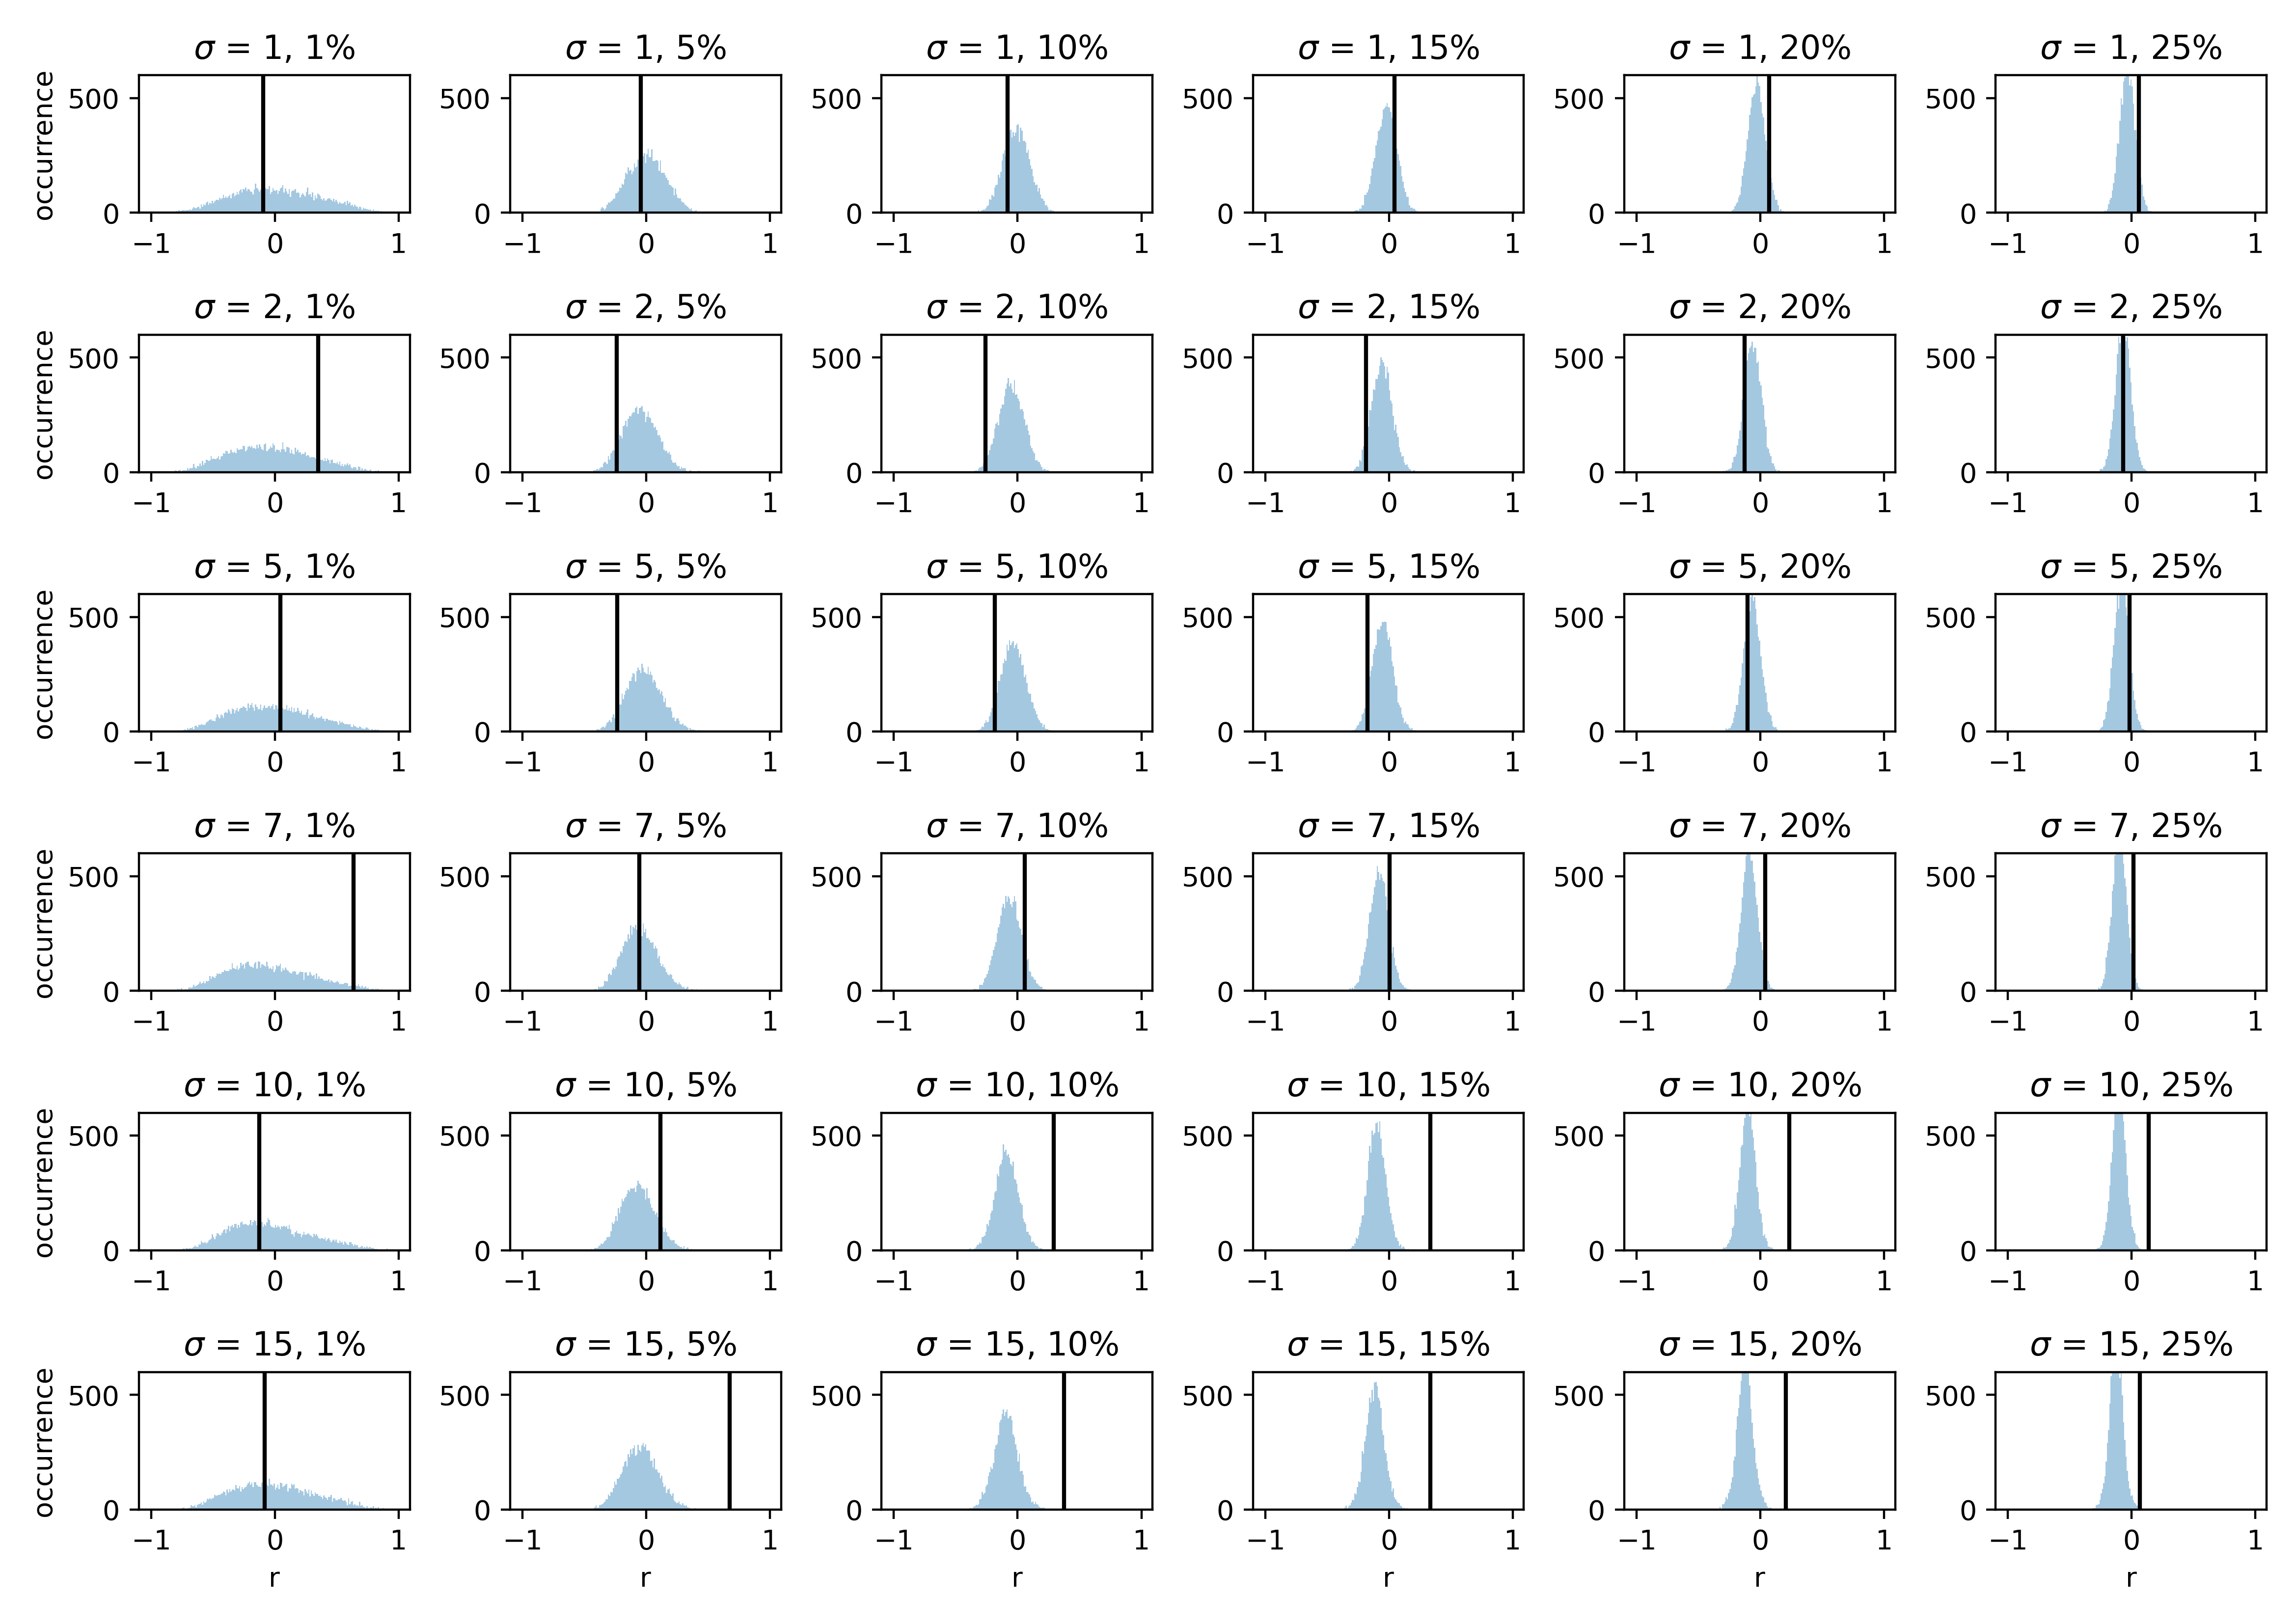
\includegraphics[width =0.9\linewidth]{Figures/Figures-surface/cors_sigs_thresh_and_sigma_weak.png} 
\caption{like figure \ref{cors_stats_parameters_strong} for correlations between NAM$_{10}$ values associated with persistent weak intervals and 17 year lagged AMOC anomalies at 50N.}
\label{cors_stats_parameters_weak}
\end{center}
\end{figure}
\end{landscape}

%%% Local Variables:
%%% mode: latex
%%% TeX-master: "thesis"
%%% End:

\section{Summary and Discussion}

In this chapter we analyse the influence of persistent polar vortex extremes, intervals which exhibit either consecutive weak or strong vortex winters, on surface and ocean circulation in a 1000 year pi-control simulation of UKESM. Persistent vortex anomalies are identified using a smoothed NAM$_{10}$ index which characterises intervals of approximately 6-8 years during which the NH winter vortex is anomalously strong (positive NAM$_{10}$ anomaly) or weak (negative NAM$_{10}$ anomaly). While the surface impacts of stratospheric extremes in individual winters (such as sudden stratospheric warmings) has received much attention \citep{baldwinStratospheric2001a, domeisenEstimating2019, charlton-perezInfluence2018a} the surface impacts of persistently anomalous winters has been less well studied and  teleconnections between the stratospheric vortex and ocean variability are not well characterised or understood. 

We examine the AMOC response to long-term variations in the stratospheric polar vortex using composite analysis of the AMOC strength following persistent anomalous NAM$_{10}$ intervals. We find oscillatory responses (figure \ref{NAO_AMOC_T_response}) from the NAO and the AMOC consistent with previous work  \citep{reichlerStratospheric2012}. We propose that this behaviour is due to a combination of effects. Firstly, resonant oscillatory signals in the NAM$_{10}$ and the AMOC which involve the ocean's natural modes of oscillation being amplified due to integrated forcing from the atmosphere (originating from the vortex) varying on a similar timescale. Secondly, through feedbacks between the NAO, which is initially perturbed by the NAM, and the AMOC in which the NAO signal is able to penetrate into the deep ocean thermocline which subsequently forces and then responds to the AMOC. This induces a change in the NAO phase which damps the AMOC response.

We also find that different types of persistent vortex intervals are associated with different AMOC patterns in the simulation. Namely, strong intervals lead to oscillatory responses of near 30 year periods with peaks in the NAM$_{10}$ leading those in the AMOC by approximately 2-4 years. Meanwhile, weak intervals associate with longer timescale (50-100 years) variations in the ocean with the extremes in the AMOC appearing both before and after peaks in the persistent NAM. We aim to understand these differences by considering the vortex behaviour under strong and weak conditions, i.e. weak winters will only influence the surface once an SSW occurs, while strong winters act through the whole season. Whilst this represents an asymmetric forcing, just how this accounts for different AMOC response timescales is unclear. We additionally found prominent signal non-stationarities across multiple timescales in the AMOC, NAO and NAM$_{10}$. Wavelet analysis reveals 3 intervals during which 30, 50 and 90 year periodic behaviour is present in the NAM$_{10}$ and AMOC, 2 of which (those at 50 and 30 year periods) also feature similar signals in the NAO. We therefore propose that the composite response patterns seen in this analysis are the superposition of contributions from intervals exhibiting different timescale behaviour. The distribution of different persistent vortex interval types relative to these intervals therefore accounts for the different AMOC behaviour associated with them: a large proportion of strong intervals are situated within the 30 year timescale interval while a higher proportion of weak intervals occur during the 50 and 90 year timescale intervals. On the 90 year timescale we show that signals in the vortex are associated with similar variations in tropical east Pacific deep convection and QBO amplitude. The AMOC also appears to co-vary with the rate of change of such tropical convection also with 90 year periods completing a possible novel AMOC pathway to influence the strength of the vortex.

We subsequently assess the relationship between the magnitude of the strong persistent NAM$_{10}$ intervals and the resulting AMOC anomalies. This analysis suggests that the magnitude of filtered NAM$_{10}$ extremes, which captures both the strength of anomalous vortex behaviour as well as the persistence of the same type of behaviour in an approximately 6-8 year window, is directly proportional to the AMOC anomaly 17 years later. This relationship is shown to display a remarkable degree of correlation ($r = 0.908$). We finally use this relationship to estimate the contribution of the persistent strong interval of the 1990s, which appears in observations, on recent AMOC trends. This method predicts a -0.89Sv anomaly in the AMOC due to the due to persistent strong vortex behaviour during the 1990s.

This final finding is a striking, novel result: -0.89Sv represents nearly 30\% of the total decrease in AMOC transport between 2005 and 2013 which has been primarily attributed to anthropogenic forcing factors \citep{caesarObserved2018, caesarCurrent2021}. In contrast, NH vortex variability is largely regarded as a mode of internal variability within the climate system - there is no consensus amongst GCMs as to the response from the vortex to anthropogenic forcings \citep{ayarzaguenaUncertainty2020}. As a result, our findings may indicate a significant role of internally generated signals in recent observations of the AMOC. However, The result relies on a number of key assumptions: First, we assume that the relationship between strong persistent NAM$_{10}$ intervals and the AMOC holds in the real climate system. As the connection proposed is not well explored in previous literature, there is limited analysis on the ability of GCM's to represent vortex-AMOC interactions (\cite{reichlerStratospheric2012} showed some interaction in CMIP5 models). However, some studies report that GCMs under-represent the influence of SSW events on the jet, NAO and surface temperatures in the form of the so called "signal to noise" problem in which stratospheric signals in GCMs fail to emerge above noise in tropospheric variability \citep{scaifeSignaltonoise2018}. Such an issue does not appear to emerge in UKESM however as a clear NAO signal is apparent up to 3 months following events (figure \ref{fig:surface_comp_all} top row) indicating that reasonable connection between the stratosphere and the surface is present in the simulation and that connections with the AMOC may also be realistic. 

Second, the interaction between persistent vortex intervals and the AMOC in the simulation appears to be heavily weighted towards the interval in which 30 year timescale variations in both modes dominate. This variability is a non-stationary feature which persists for approximately 70-100 years of the 1000 year simulation. We therefore assume that such variability is also realistic within the observational record and the validity of this assumption may rely on whether such an interval is present in the real climate system. If we consider the pi-control simulation as a realisation of the real climate system over an arbitrary 1000 year interval, we can estimate the probability of the emergence of such intervals as 0.07-0.10 as 30 year variations appeared for 70-100 years in the 1000 year simulation. This suggests 30 year timescale variations are most likely not present in the observations. However, the linear relationship between NAM$_{10}$ extreme magnitude and AMOC anomaly is established from the whole simulation suggesting that connection is not solely confined to 30 year variations despite the heavy weighting towards intervals exhibiting this frequency variability.

Overall, results from this chapter suggest a novel, non-stationary interaction between the vortex and Atlantic circulation as well as suggest a possible key role for the stratosphere in recent AMOC observations. Key limitations to the analysis presented here as well as further work following on from this study is explored in section \ref{sec:limitations}.






